\documentclass[dvipdfmx,10pt]{beamer}
\bibliographystyle{junsrt}
\setbeamertemplate{navigation symbols}{}
\setbeamertemplate{footline}[frame number] 
\usepackage{graphicx}
\usepackage{minijs}%和文用
\renewcommand{\kanjifamilydefault}{\gtdefault}%和文用
\usetheme{EastLansing}
\usepackage{tikz}
\usepackage{xspace}
\usepackage{comment}
\usepackage{hyperref}
\usepackage{otf}
%\usefonttheme{serif}
\usepackage{ascmac}
%\usepackage[absolute,overlay]{textpos}
%\usefonttheme{professionalfonts}
\usepackage{amsmath}
\usepackage{caption}

\usetikzlibrary{lindenmayersystems}
\usetikzlibrary{shapes,arrows}

\usetikzlibrary{positioning,automata}
\usetikzlibrary{decorations.markings}
\usepackage{mathtools}
\usepackage{geometry}
\usetikzlibrary{%
  arrows,%
  positioning,%
  decorations.pathmorphing,%
  decorations.pathreplacing,%
}






\setlength{\columnsep}{3zw}
\makeatletter
\def\presentation#1{\def\@presentation{#1}}
\def\@maketitle{
\begin{flushright}
{\large \@date}% 日付 
\end{flushright}
\begin{center}
{\large \@presentation}% 会名 
\end{center}% 
\begin{center} 
{\LARGE \@title \par}% タイトル 
\end{center}
\begin{center} 
{\large \@author}% 著者 

\end{center}
\par\vskip 1.5em
}
\makeatother

%\beamersetuncovermixins{\opaqueness<1>{25}}{\opaqueness<2->{15}}
\begin{document}
\title{Towards the algorithmic molecular self-assembly of fractals \\by cotranscriptional folding} 
\author{Yusei Masuda, Shinnosuke Seki, and Yuki Ubukata}
\institute{University of Electro-Communications Tokyo}
\date{July 30th, 2018}
\begin{frame}
\maketitle
\end{frame}

%%%%%%%%%%%%%%%%%%%%%%%%%%%%%%%%%%%%%%%%%%%%%%%%%%%%%%%%
\section{Introduction}
\begin{frame}\frametitle{Cotranscriptional folding}
\begin{itemize}
\item Cotranscriptional folding--folding occurs during transcription
%\item RNA Origami (Geary et al. (2014))
\end{itemize}
\begin{figure}
\centering
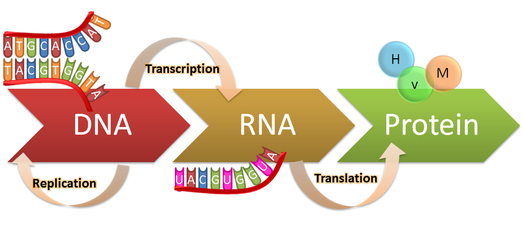
\includegraphics[width=0.7\linewidth]{central.png}
\caption{Central dogma--Information flow in biological systems.}
\end{figure}

\end{frame}
%%%%%%%%%%%%%%%%%%%%%%%%%%%%%%%%%%%%%%%%%%%%%%%%%%%%%%%%%
%
%\begin{frame}
%\begin{tikzpicture}
%\node[rectangle,draw] (n1) at (0, 0) {\tt A}; 
%\node[rectangle,draw] (n2) at (1, 0) {\tt T}; 
%\node[rectangle,draw] (n3) at (2, 0) {\tt C}; 
%\node[rectangle,draw] (n4) at (3, 0) {\tt G}; 
%\node[rectangle,draw] (n5) at (4, 0) {\tt C}; 
%\node[rectangle,draw] (n6) at (5, 0) {\tt A}; 
%\node[rectangle,draw] (n7) at (6, 0) {\tt T}; 
%\node[rectangle,draw] (n8) at (7, 0) {\tt C}; 
%\node[rectangle,draw] (n9) at (8, 0) {\tt G}; 
%
%\draw[very thick] (n1) -- (n2) -- (n3) -- (n4) -- (n5) -- (n6) -- (n7) -- (n8) -- (n9); 
%\node at (4,-1) {Template DNA sequence}; %%%%%%%%
%
%
%\uncover<1>{\fill [orange!50, opacity=.5] (2, 3) circle [x radius=1cm, y radius=2cm] node [orange,opacity=1] {T7 RNA polymerase};} 
%\uncover<2>{
%	\fill [orange!50, opacity=.5] (0, 2) circle [x radius=1cm, y radius=2cm] node [orange,opacity=1] {T7 RNA polymerase};
%	\node[circle,color=blue] at (1,3) {\tt U}; 
%} 
%\uncover<3>{
%	\fill [orange!50, opacity=.5] (1, 2) circle [x radius=1cm, y radius=2cm] node [orange,opacity=1] {T7 RNA polymerase};
%	\node[circle,color=blue] (r21) at (2.8,3.6) {\tt U}; 
%	\node[circle,color=blue] (r22) at (2,3) {\tt A}; 
%	\draw[blue,thick] (r22) to [out=30,in=210] (r21); 
%} 
%\uncover<4>{
%	\fill [orange!50, opacity=.5] (2, 2) circle [x radius=1cm, y radius=2cm] node [orange,opacity=1] {T7 RNA polymerase};
%	\node[circle,color=blue] (r31) at (4.6,4.2) {\tt U}; 
%	\node[circle,color=blue] (r32) at (3.8,3.6) {\tt A}; 
%	\node[circle,color=blue] (r33) at (3,3) {\tt G}; 
%	\draw[blue,thick] (r33) to [out=30,in=210] (r32);
%	\draw[blue,thick] (r32) to [out=30,in=210] (r31); 
%} 
%\uncover<5>{
%	\fill [orange!50, opacity=.5] (3, 2) circle [x radius=1cm, y radius=2cm] node [orange,opacity=1] {T7 RNA polymerase};
%	\node[circle,color=blue] (r41) at (6.5,4.1) {\tt U}; 
%	\node[circle,color=blue] (r42) at (5.6,4.2) {\tt A}; 
%	\node[circle,color=blue] (r43) at (4.8,3.6) {\tt G}; 
%	\node[circle,color=blue] (r44) at (4,3) {\tt C}; 
%	\draw[blue,thick] (r44) to [out=30,in=210] (r43);
%	\draw[blue,thick] (r43) to [out=30,in=210] (r42); 
%	\draw[blue,thick] (r42) to [out=30,in=150] (r41); 
%} 
%\uncover<6>{
%	\fill [orange!50, opacity=.5] (4, 2) circle [x radius=1cm, y radius=2cm] node [orange,opacity=1] {T7 RNA polymerase};
%	\node[circle,color=blue] (r51) at (7.9,3.3) {\tt U}; 
%	\node[circle,color=blue] (r52) at (7.5,4.1) {\tt A}; 
%	\node[circle,color=blue] (r53) at (6.6,4.2) {\tt G}; 
%	\node[circle,color=blue] (r54) at (5.8,3.6) {\tt C}; 
%	\node[circle,color=blue] (r55) at (5,3) {\tt G}; 
%	\draw[blue,thick] (r55) to [out=30,in=210] (r54);
%	\draw[blue,thick] (r54) to [out=30,in=210] (r53); 
%	\draw[blue,thick] (r53) to [out=30,in=150] (r52); 
%	\draw[blue,thick] (r52) to [out=300,in=120] (r51); 
%} 
%\uncover<7>{
%	\fill [orange!50, opacity=.5] (5, 2) circle [x radius=1cm, y radius=2cm] node [orange,opacity=1] {T7 RNA polymerase};
%	\node[circle,color=blue] (r61) at (8.1,2.4) {\tt U}; 
%	\node[circle,color=blue] (r62) at (8.5,3.1) {\tt A}; 
%	\node[circle,color=blue] (r63) at (8.5,4.1) {\tt G}; 
%	\node[circle,color=blue] (r64) at (7.6,4.2) {\tt C}; 
%	\node[circle,color=blue] (r65) at (6.8,3.6) {\tt G}; 
%	\node[circle,color=blue] (r66) at (6,3) {\tt U}; 
%	\draw[blue,thick] (r66) to [out=30,in=210] (r65);
%	\draw[blue,thick] (r65) to [out=30,in=210] (r64); 
%	\draw[blue,thick] (r64) to [out=30,in=150] (r63); 
%	\draw[blue,thick] (r63) to [out=285,in=75] (r62); 
%	\draw[blue,thick] (r62) to [out=270,in=30] (r61); 
%} 
%\uncover<8>{
%	\fill [orange!50, opacity=.5] (6, 2) circle [x radius=1cm, y radius=2cm] node [orange,opacity=1] {T7 RNA polymerase};
%	\node[circle,color=blue] (r71) at (7.7,2.3) {\tt U}; 
%	\node[circle,color=blue] (r72) at (8.5,2.9) {\tt A}; 
%	\node[circle,color=blue] (r73) at (9.5,3.1) {\tt G}; 
%	\node[circle,color=blue] (r74) at (9.5,4.1) {\tt C}; 
%	\node[circle,color=blue] (r75) at (8.6,4.2) {\tt G}; 
%	\node[circle,color=blue] (r76) at (7.8,3.6) {\tt U}; 
%	\node[circle,color=blue] (r77) at (7,3) {\tt A}; 
%	\draw[blue,thick] (r77) to [out=30,in=210] (r76);
%	\draw[blue,thick] (r76) to [out=30,in=210] (r75); 
%	\draw[blue,thick] (r75) to [out=30,in=150] (r74); 
%	\draw[blue,thick] (r74) to [out=285,in=75] (r73); 
%	\draw[blue,thick] (r73) to [out=210,in=0] (r72); 
%	\draw[blue,thick] (r72) to [out=210,in=45] (r71); 
%	\draw[dotted,blue,thick] (r77) -- (r71); \draw[dotted,blue,thick] (r76) -- (r72); 
%} 
%\uncover<9->{
%	\fill [orange!50, opacity=.5] (8, 2) circle [x radius=1cm, y radius=2cm] node [orange,opacity=1] {T7 RNA polymerase};
%	\node[circle,color=blue] (r89) at (9,3) {\tt C}; 
%	\node[circle,color=blue] (r88) at (9.1,3.7) {\tt G}; 
%	\node[circle,color=blue] (r87) at (8.6,4.3) {\tt A}; 
%	\node[circle,color=blue] (r86) at (8.6,5.2) {\tt U}; 
%	\node[circle,color=blue] (r85) at (8.3,6.1) {\tt G}; 
%	\node[circle,color=blue] (r84) at (9.1,6.4) {\tt C}; 
%	\node[circle,color=blue] (r83) at (9.9,6.1) {\tt G}; 
%	\node[circle,color=blue] (r82) at (9.6,5.2) {\tt A}; 
%	\node[circle,color=blue] (r81) at (9.6,4.3) {\tt U}; 
%
%	\draw[blue,thick] (r89) to [out=30, in=315] (r88); 
%	\draw[blue,thick] (r88) to [out=135, in=300] (r87); 
%	\draw[blue,thick] (r87) -- (r86); 
%	\draw[blue,thick] (r86) to [out=120, in=270] (r85); 
%	\draw[blue,thick] (r85) -- (r84) -- (r83); 
%	\draw[blue,thick] (r83) to [out=270, in=60] (r82); 
%	\draw[blue,thick] (r82) -- (r81); 
%
%	\draw[dotted,blue,thick] (r86) -- (r82); 
%	\draw[dotted,blue,thick] (r87) -- (r81); 
%}
%\uncover<10->{
%	\node[circle,color=blue] (c9) at (2, 4) {\tt C}; 
%	\node[circle,color=blue] (c8) at (2, 4.9) {\tt G}; 
%	\node[circle,color=blue] (c7) at (1.7, 5.8) {\tt A}; 
%	\node[circle,color=blue] (c6) at (2.5, 6.1) {\tt U}; 
%	\node[circle,color=blue] (c5) at (3.3, 5.8) {\tt G}; 
%	\node[circle,color=blue] (c4) at (3, 4.9) {\tt C}; 
%	\node[circle,color=blue] (c3) at (3, 4) {\tt G}; 
%	\node[circle,color=blue] (c2) at (3.4, 3.2) {\tt A}; 
%	\node[circle,color=blue] (c1) at (4, 3.8) {\tt U}; 
%
%	\draw[blue,thick] (c9) -- (c8); 
%	\draw[blue,thick] (c8) to [out=120, in=270] (c7); 
%	\draw[blue,thick] (c7) -- (c6) -- (c5); 
%	\draw[blue,thick] (c5) to [out=270, in=60] (c4); 
%	\draw[blue,thick] (c4) -- (c3);
%	\draw[blue,thick] (c3) to [out=270,in=135] (c2); 
%	\draw[blue,thick] (c2) to [out=330,in=270] (c1); 
%
%	\draw[dotted,blue,thick] (c8) -- (c4); 
%	\draw[dotted,blue,thick] (c9) -- (c3); 
%
%	\node at (2.5, 2.5) {(For reference) folding with minimum free energy}; %%%%%%%%%%%
%}
%\end{tikzpicture}
%
%
%
%\end{frame}
%%%%%%%%%%%%%%%%%%%%%%%%%%%%%%%%%%%%%%%%%%%%%%%%%%%%%%%%%%%%%%%%%%
\frame{
\frametitle{Cotranscriptional folding}
\framesubtitle{RNA polymerase}

\centering
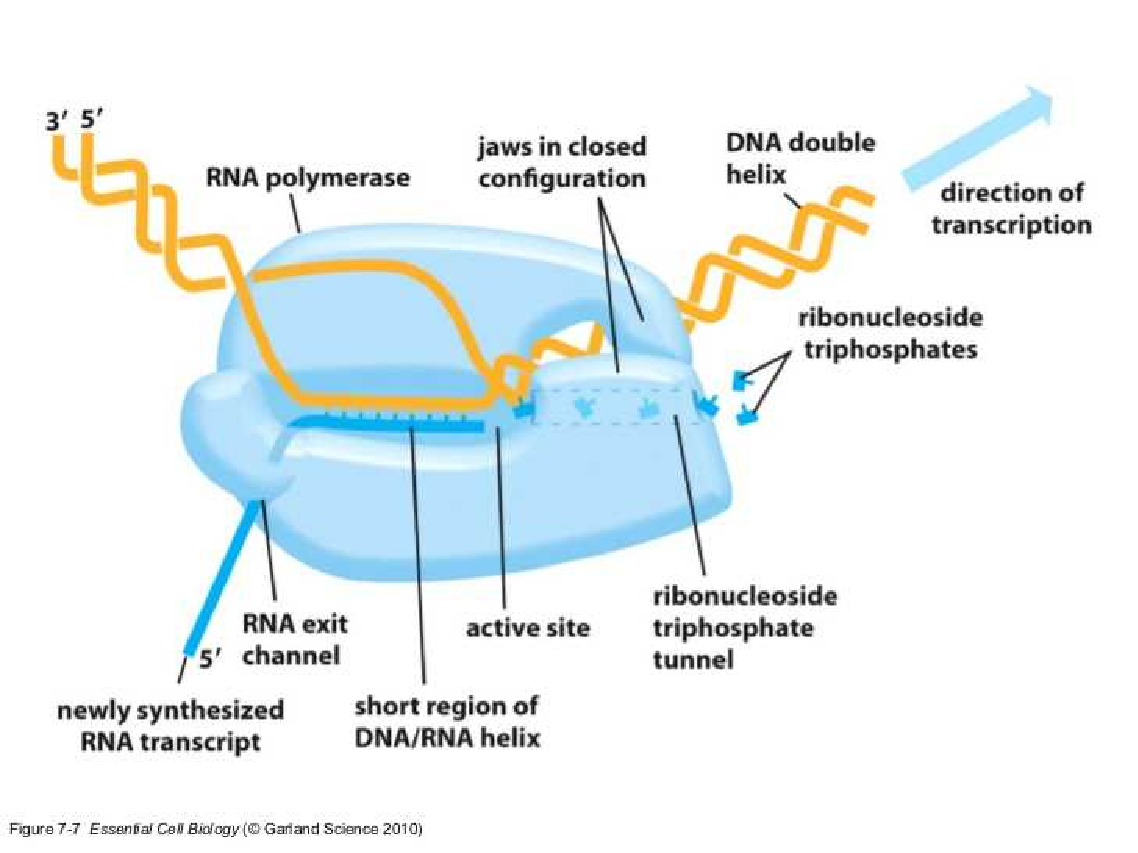
\includegraphics[width=0.7\linewidth]{rna_polymerase.pdf}
}%frame

%%%%%%%%%%%%%%%%%%%%%%%%%%%%%%%%%%%%%%%%%%%%%%%%%%%%%%%%%%%%%%%%%%

\begin{frame}\frametitle{Cotranscriptional folding}
\framesubtitle{RNA Origami \scriptsize{\cite{Geary2014}}}

\begin{figure}
\centering
\href{run:CF.mp4}{
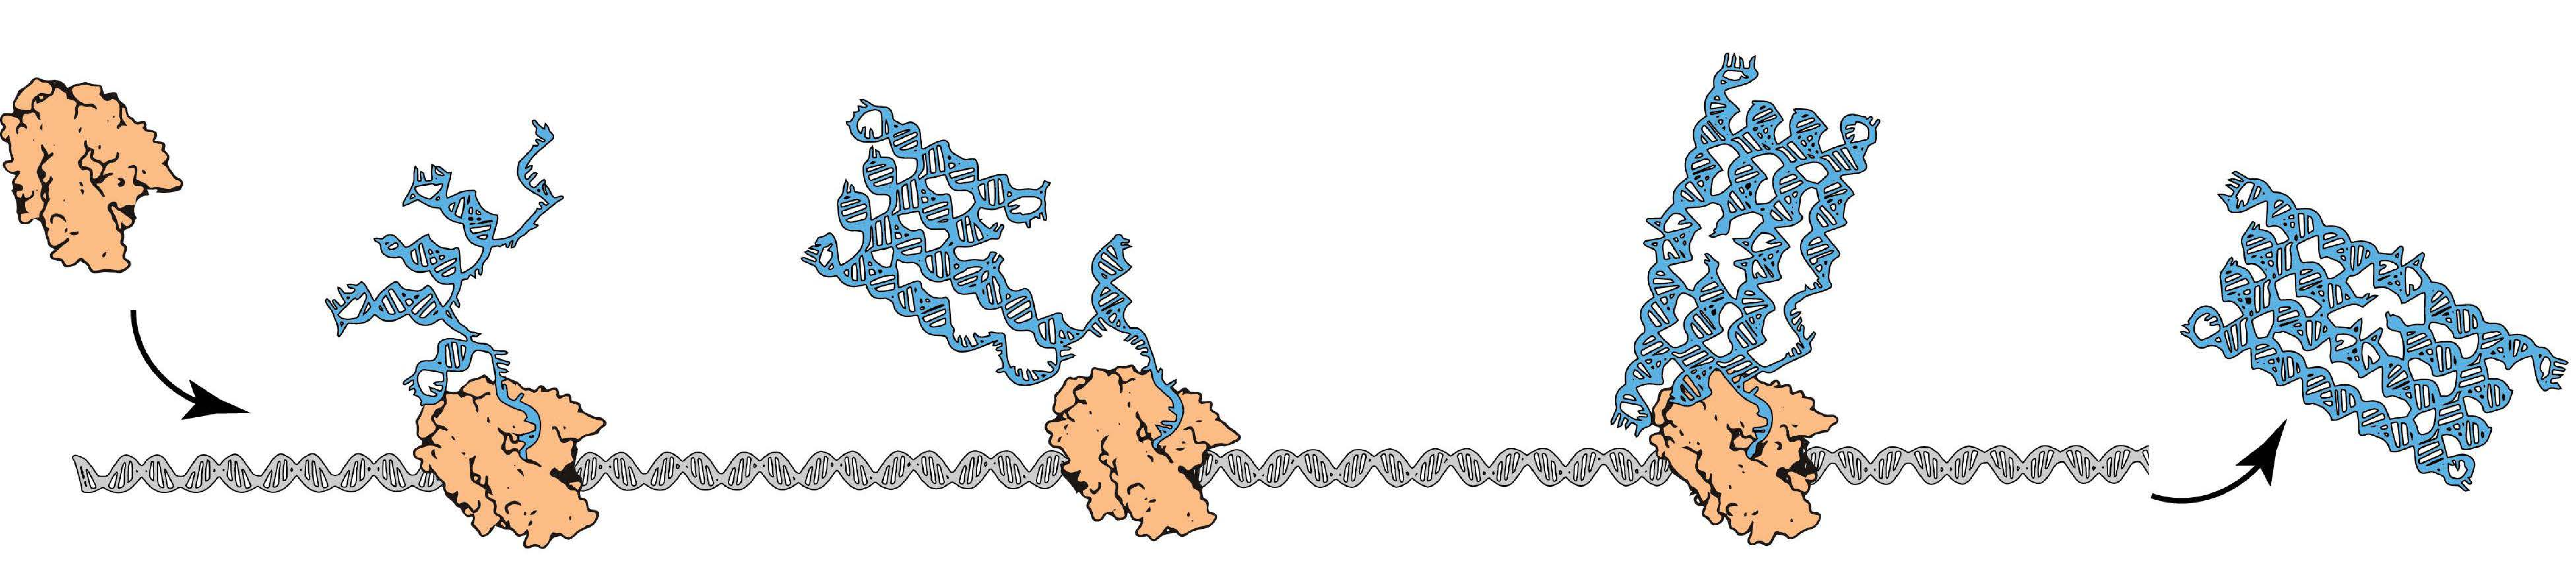
\includegraphics[width=\linewidth]{rna_origami.pdf}
}
\caption{Design of ssRNA origami that self-assembles RNA tiles.}
\end{figure}
\end{frame}

%%%%%%%%%%%%%%%%%%%%%%%%%%%%%%%%%%%%%%%%%%%%%%%%%%%%%%%%%%%%%%%%%%

\frame{
\frametitle{Cotranscriptional folding}
\framesubtitle{Regulation in gene expression by CF {\footnotesize \cite{Watters2016}}}

Transcript: {\scriptsize \texttt{UUAUAGGCGAUGGAGUUCGCCAUAAACGCUGCUUAGCUAAU\textcolor{red}{GACUCCUACCAGUAUCACUACUGGUAGGAGUC}}}

\vspace*{5mm}

%Possible conformations: \\
{\footnotesize Concentration of NaF may promote or inhibit the transcript above to fold into the \textcolor{red}{terminator stem} cotranscriptionally.}

\vspace*{3mm}

\begin{minipage}{0.45\linewidth}


\centering

\scalebox{0.7}{\begin{tikzpicture}

\draw (0, 0) node {\tt U}
++(0:0.2) node {\tt U}
++(0:0.2) node {\tt A}
++(0:0.2) node {\tt U}
++(0:0.2) node {\tt A}
++(0:0.2) node(Q1-1) {\tt G}
++(90:0.3) node(Q1-2) {\tt G}
++(90:0.3) node(Q1-3) {\tt C}
++(90:0.3) node(Q1-4) {\tt G}
++(90:0.3) node(Q1-5) {\tt A}
++(120:0.3) node {\tt A}
++(80:0.3) node {\tt G}
++(40:0.3) node {\tt G}
++(0:0.3) node {\tt A}
++(320:0.3) node {\tt G}
++(280:0.3) node {\tt U}
++(240:0.3) node(Q1-5*) {\tt U}
++(270:0.3) node(Q1-4*) {\tt C}
++(270:0.3) node(Q1-3*) {\tt G}
++(270:0.3) node(Q1-2*) {\tt C}
++(270:0.3) node(Q1-1*) {\tt C}
++(0:0.2) node {\tt A}
++(0:0.2) node {\tt U}
++(0:0.2) node {\tt A}
++(0:0.2) node {\tt A}
++(0:0.2) node {\tt A}
++(0:0.2) node {\tt C}
++(0:0.2) node(Q3-1) {\tt G}
++(90:0.3) node(Q3-2) {\tt C}
++(90:0.3) node(Q3-3) {\tt U}
++(105:0.3) node {\tt G}
++(45:0.3) node {\tt C}
++(0:0.3) node {\tt U}
++(315:0.3) node {\tt U}
++(255:0.3) node(Q3-3*) {\tt A}
++(270:0.3) node(Q3-2*) {\tt G}
++(270:0.3) node(Q3-1*) {\tt C}
++(0:0.2) node {\tt U}
++(0:0.2) node {\tt A}
++(0:0.2) node {\tt A}
++(0:0.2) node {\tt U}
++(0:0.2) node(T1-1) [red] {\tt G}
;

\draw[red] (T1-1)
++(90:0.3) node(T1-2) {\tt A}
++(90:0.3) node(T1-3) {\tt C}
++(90:0.3) node(T1-4) {\tt U}
++(90:0.3) node(T1-5) {\tt C}
++(90:0.3) node(T1-6) {\tt C}
++(90:0.3) node(T1-7) {\tt U}
++(90:0.3) node(T1-8) {\tt A}
++(90:0.3) node(T1-9) {\tt C}
++(90:0.3) node(T1-10) {\tt C}
++(90:0.3) node(T1-11) {\tt A}
++(90:0.3) node(T1-12) {\tt G}
++(90:0.3) node(T1-13) {\tt U}
++(90:0.3) node(T1-14) {\tt A}
++(105:0.3) node {\tt U}
++(45:0.3) node {\tt C}
++(0:0.3) node {\tt A}
++(315:0.3) node {\tt C}
++(255:0.3) node(T1-14*) {\tt U}
++(270:0.3) node(T1-13*) {\tt A}
++(270:0.3) node(T1-12*) {\tt C}
++(270:0.3) node(T1-11*) {\tt U}
++(270:0.3) node(T1-10*) {\tt G}
++(270:0.3) node(T1-9*) {\tt G}
++(270:0.3) node(T1-8*) {\tt U}
++(270:0.3) node(T1-7*) {\tt A}
++(270:0.3) node(T1-6*) {\tt G}
++(270:0.3) node(T1-5*) {\tt G}
++(270:0.3) node(T1-4*) {\tt A}
++(270:0.3) node(T1-3*) {\tt G}
++(270:0.3) node(T1-2*) {\tt U}
++(270:0.3) node(T1-1*) {\tt C}
;

\draw
(Q1-1) -- (Q1-1*)
(Q1-2) -- (Q1-2*)
(Q1-3) -- (Q1-3*)
(Q1-4) -- (Q1-4*)
(Q1-5) -- (Q1-5*)
;

\draw
(Q3-1) -- (Q3-1*)
(Q3-2) -- (Q3-2*)
(Q3-3) -- (Q3-3*)
;

\draw
(T1-1) -- (T1-1*)
(T1-2) -- (T1-2*)
(T1-3) -- (T1-3*)
(T1-4) -- (T1-4*)
(T1-5) -- (T1-5*)
(T1-6) -- (T1-6*)
(T1-7) -- (T1-7*)
(T1-8) -- (T1-8*)
(T1-9) -- (T1-9*)
(T1-10) -- (T1-10*)
(T1-11) -- (T1-11*)
(T1-12) -- (T1-12*)
(T1-13) -- (T1-13*)
(T1-14) -- (T1-14*)
;

\end{tikzpicture}}

{\scriptsize Terminated (0 mM NaF)}

\end{minipage}
\begin{minipage}{0.05\linewidth}
\ \\
\end{minipage}
\begin{minipage}{0.45\linewidth}

\centering

\scalebox{0.7}{\begin{tikzpicture}

\draw[thick] (0, 0) node {\tt U}
++(270:0.3) node {\tt U}
++(270:0.3) node {\tt A}
++(270:0.3) node {\tt U}
++(270:0.3) node {\tt A}
++(300:0.3) node(P1-1) {\tt G}
++(300:0.3) node(P1-2) {\tt G}
++(300:0.3) node(P1-3) {\tt C}
++(300:0.3) node(P1-4) {\tt G}
-- ++(225:0.3) node {\tt A}
++(270:0.3) node {\tt U} 
to [out=270, in=180] ++(315:1.4) node (P2-1) {\tt G}
++(90:0.3) node (P2-2) {\tt G}
++(90:0.3) node (P2-3) {\tt A}
++(90:0.3) node (P2-4) {\tt G}
++(90:0.3) node (P2-5) {\tt U}
++(90:0.3) node (P2-6) {\tt U}
++(150:0.3) node(P1-4*) {\tt C}
++(120:0.3) node(P1-3*) {\tt G}
++(120:0.3) node(P1-2*) {\tt C}
++(120:0.3) node(P1-1*) {\tt C}
++(90:0.3) node {\tt A}
++(72:0.3) node {\tt U}
++(54:0.3) node {\tt A}
++(36:0.3) node {\tt A}
++(18:0.3) node {\tt A}
++(0:0.3) node {\tt C}
++(342:0.3) node(P3-1) {\tt G}
++(30:0.3) node(P3-2) {\tt C}
++(30:0.3) node(P3-3) {\tt U}
++(45:0.3) node {\tt G}
++(0:0.3) node {\tt C}
++(315:0.4) node {\tt U}
++(255:0.4) node {\tt U}
++(195:0.3) node(P3-3*) {\tt A}
++(210:0.3) node(P3-2*) {\tt G}
++(210:0.3) node(P3-1*) {\tt C}
++(288:0.3) node {\tt U}
++(270:0.3) node {\tt A}
++(252:0.3) node {\tt A}
++(234:0.4) node {\tt U}
++(216:0.3) node(P2-6*) [red] {\tt G}
;

\draw[red] (P2-6*)
++(270:0.3) node(P2-5*) {\tt A}
++(270:0.3) node(P2-4*) {\tt C}
++(270:0.3) node(P2-3*) {\tt U}
++(270:0.3) node(P2-2*) {\tt C}
++(270:0.3) node(P2-1*) {\tt C}
++(345:0.3) node {\tt U}
++(330:0.3) node(PT-1) {\tt A}
++(60:0.3) node(PT-2) {\tt C}
++(60:0.3) node(PT-3) {\tt C}
++(60:0.3) node(PT-4) {\tt A}
++(60:0.3) node(PT-5) {\tt G}
++(60:0.3) node(PT-6) {\tt U}
++(60:0.3) node(PT-7) {\tt A}
++(75:0.3) node {\tt U}
++(15:0.3) node {\tt C}
++(330:0.3) node {\tt A}
++(285:0.3) node {\tt C}
++(225:0.3) node(PT-7*) {\tt U}
++(240:0.3) node(PT-6*) {\tt A}
++(240:0.3) node(PT-5*) {\tt C}
++(240:0.3) node(PT-4*) {\tt U}
++(240:0.3) node(PT-3*) {\tt G}
++(240:0.3) node(PT-2*) {\tt G}
++(240:0.3) node(PT-1*) {\tt U}
++(0:0.3) node {\tt A}
++(0:0.3) node {\tt G}
++(0:0.3) node {\tt G}
++(0:0.3) node {\tt A}
++(0:0.3) node {\tt G}
++(0:0.3) node {\tt U}
++(0:0.3) node {\tt C}
;

\draw (P1-1) -- (P1-1*) (P1-2) -- (P1-2*) (P1-3) -- (P1-3*) (P1-4) -- (P1-4*);

\draw (P3-1) -- (P3-1*) (P3-2) -- (P3-2*) (P3-3) -- (P3-3*);

\draw[]
(P2-1) -- (P2-1*)
(P2-2) -- (P2-2*)
(P2-3) -- (P2-3*)
(P2-4) -- (P2-4*)
(P2-5) -- (P2-5*)
(P2-6) -- (P2-6*)
;

\draw
(PT-1) -- (PT-1*)
(PT-2) -- (PT-2*)
(PT-3) -- (PT-3*)
(PT-4) -- (PT-4*)
(PT-5) -- (PT-5*)
(PT-6) -- (PT-6*)
(PT-7) -- (PT-7*)
;
\end{tikzpicture}}

{\scriptsize Antiterminated (10 mM NaF)}

\end{minipage}



}

%%%%%%%%%%%%%%%%%%%%%%%%%%%%%%%%%%%%%%%%%%%%%%%%%%%%%%%%%%%%%%%%%%

\begin{frame}\frametitle{RNA Origami \scriptsize{\cite{Geary2014}}}

\begin{figure}
\centering
\href{run:CF.mp4}{
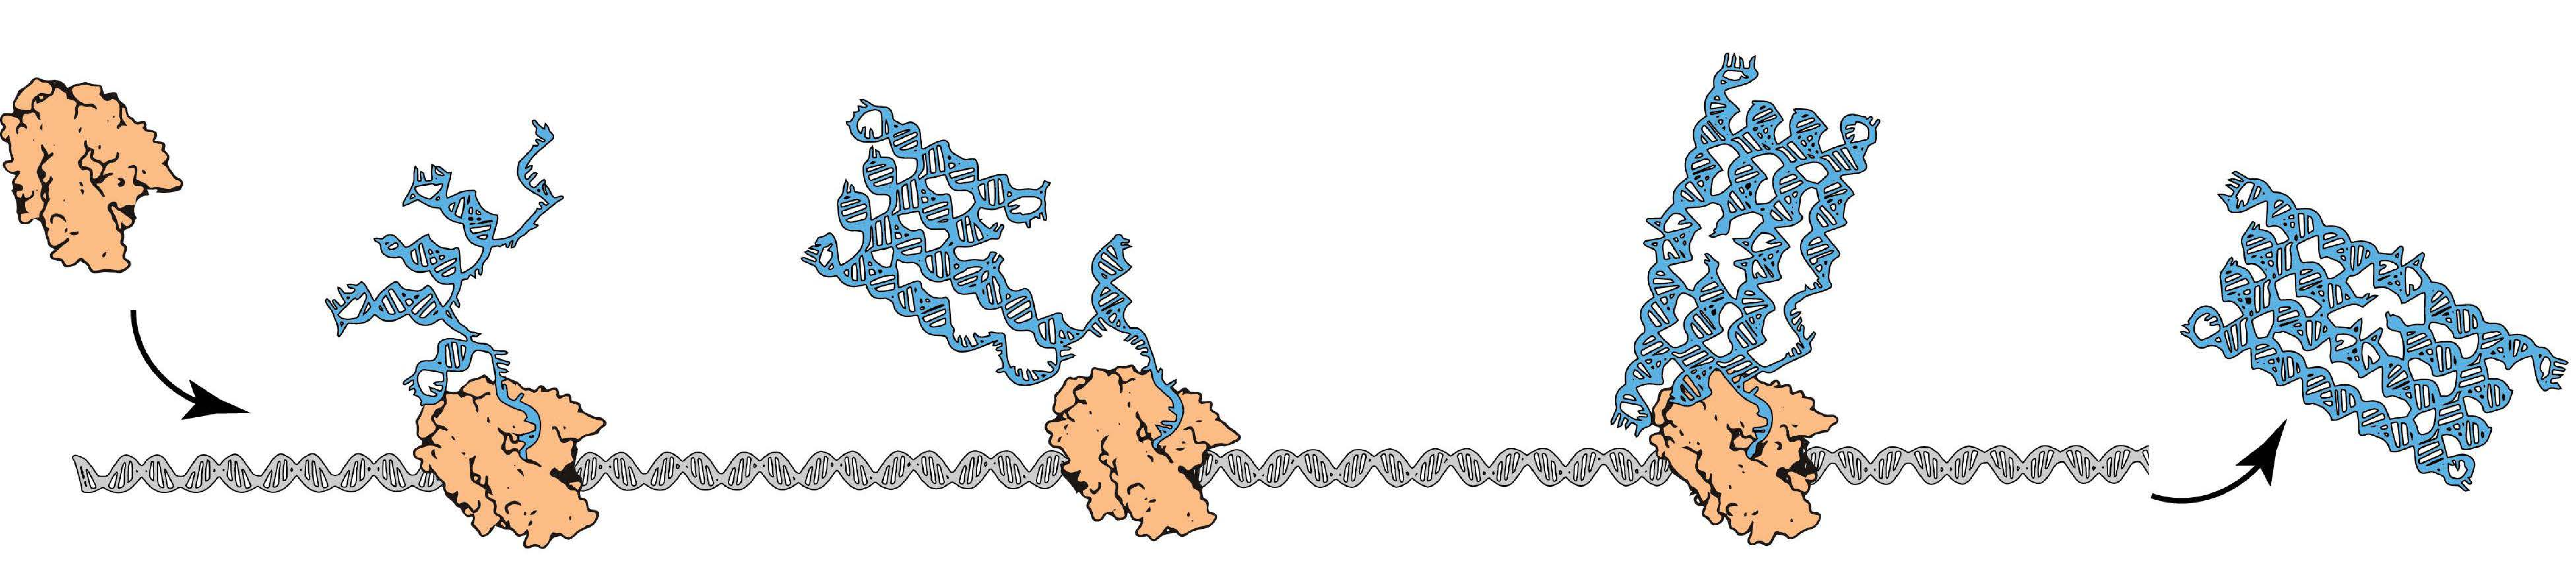
\includegraphics[width=\linewidth]{rna_origami.pdf}
}
\caption{Design of ssRNA origami that self-assembles RNA tiles.}
\end{figure}
\end{frame}
%%%%%%%%%%%%%%%%%%%%%%%%%%%%%%%%%%%%%%%%%%%%%%%%%%%%%%%%%%%%%%%%%%



\begin{frame}\frametitle{Oritatami System}
\begin{itemize}
\item Oritatami system--a mathematical model of computation by cotranscriptional folding
\end{itemize}
\begin{figure}
\centering
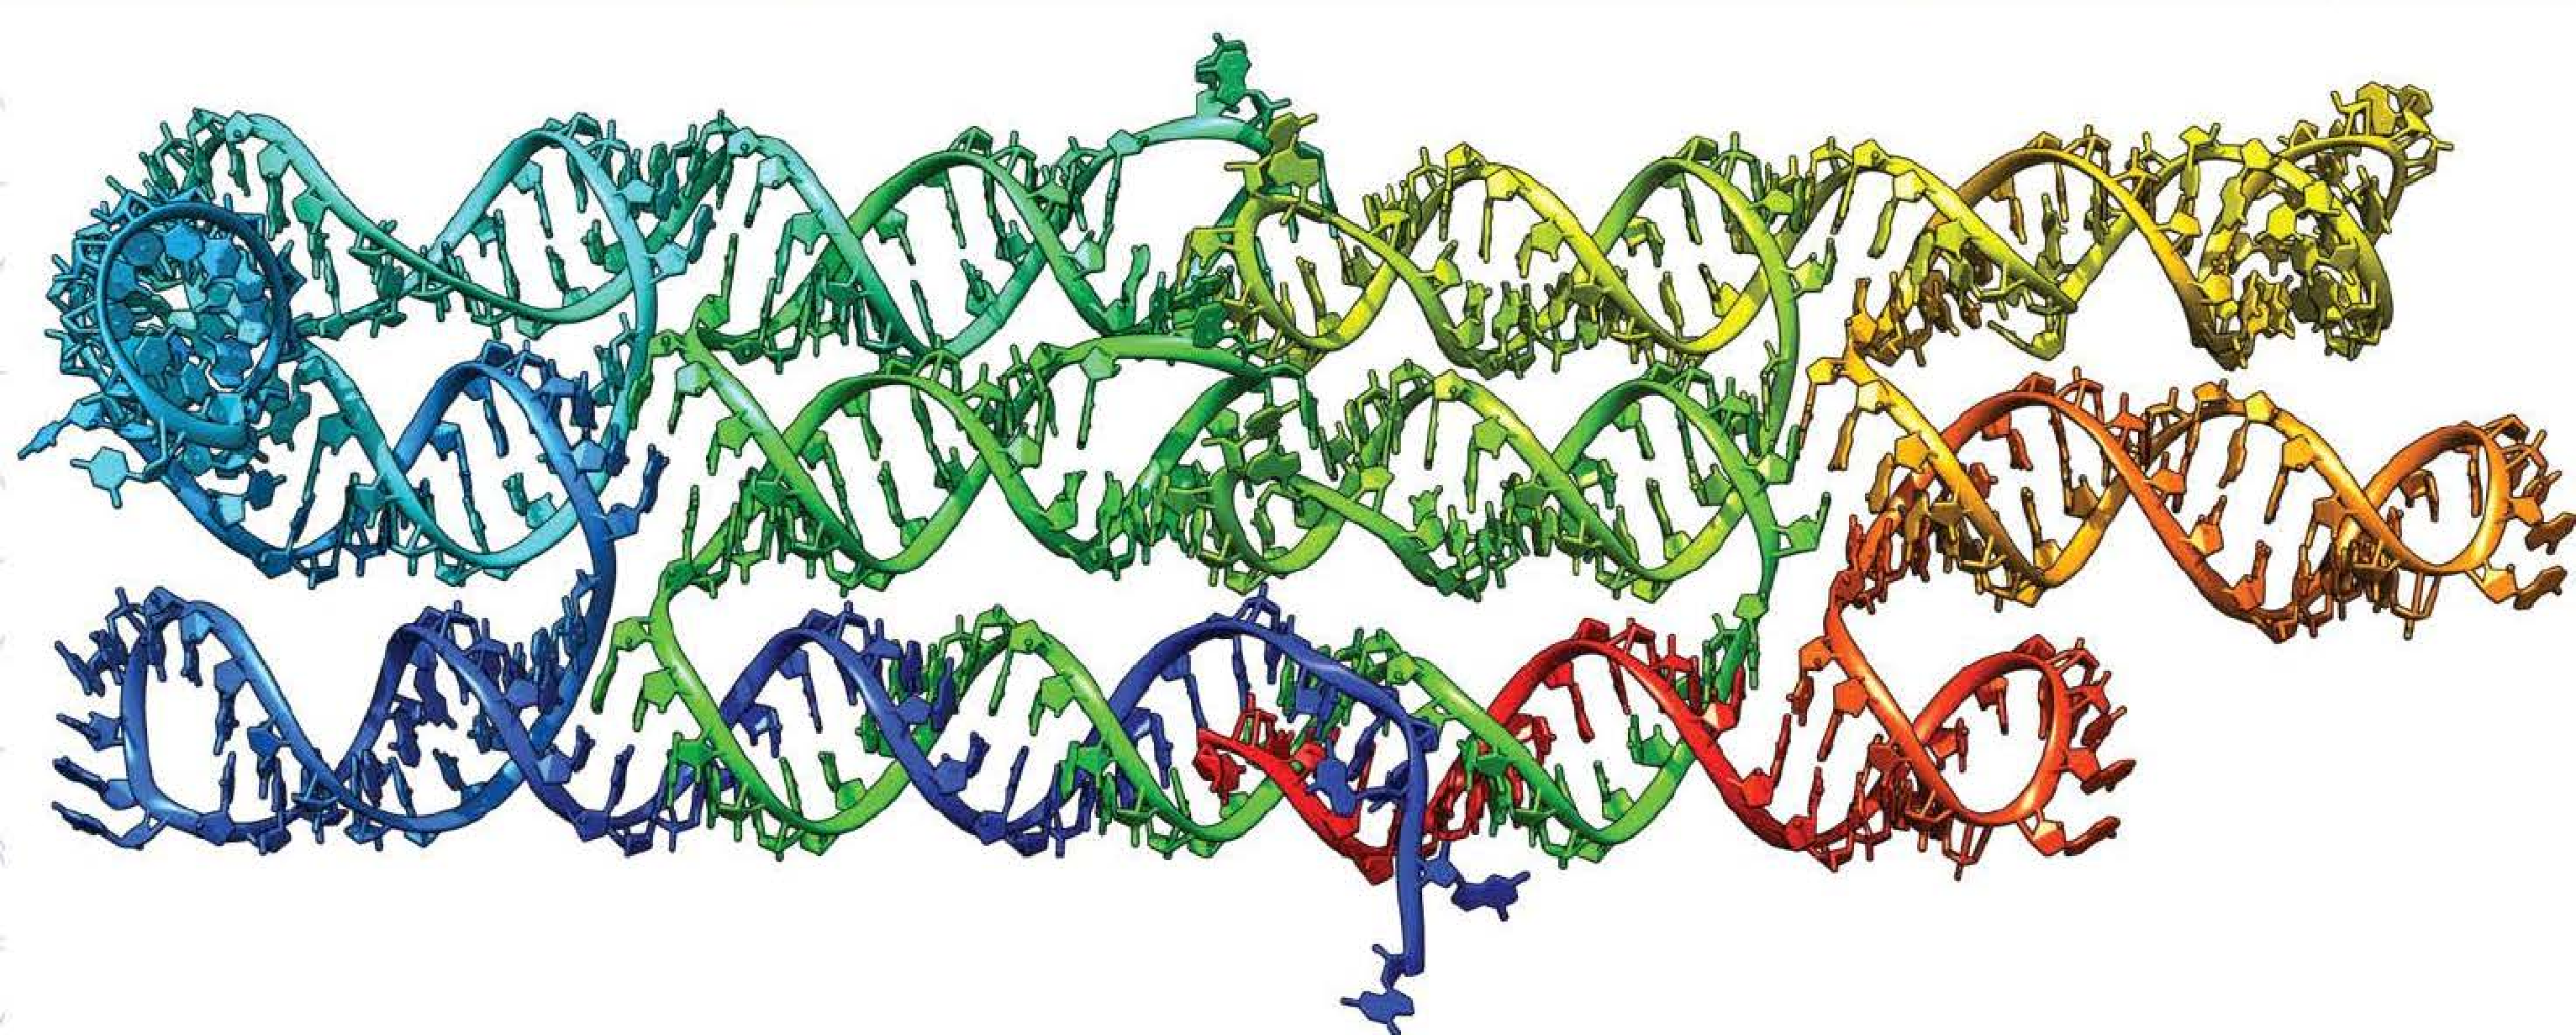
\includegraphics[width=0.6\linewidth]{rna_tile.pdf}
\end{figure}
\begin{minipage}{0.25\linewidth}
\begin{tikzpicture}
\centering
\draw[-latex,thick] (-0.5, -1) -- node[above] {abstract} ++(0:1.5);
\end{tikzpicture}
\end{minipage}
\begin{minipage}{0.6\linewidth}
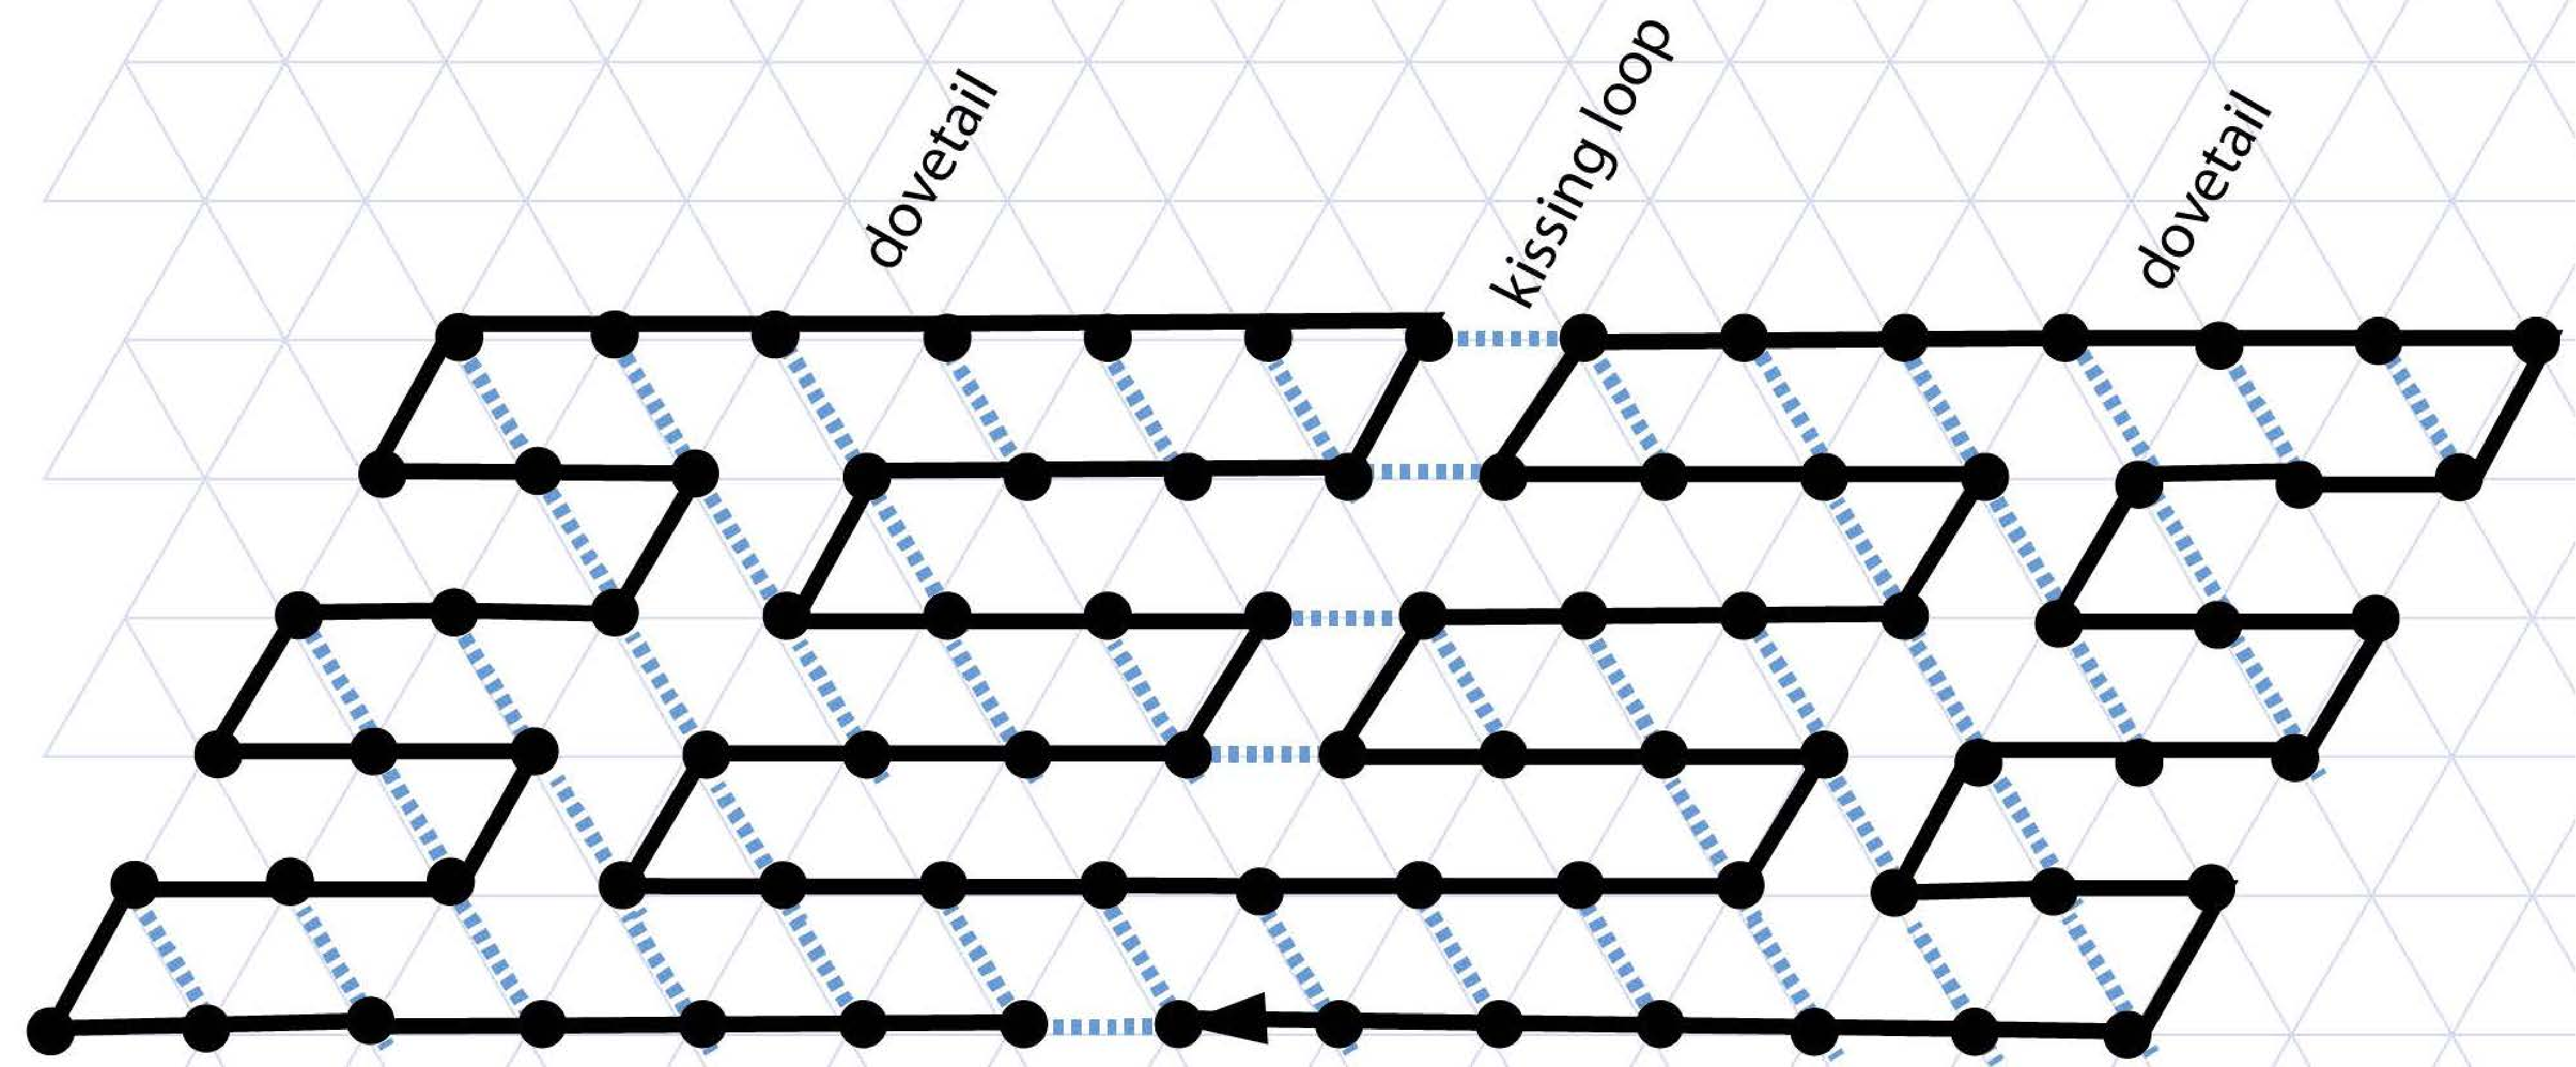
\includegraphics[width=\linewidth]{origami_oritatami.pdf}
\end{minipage}


\end{frame}
%%%%%%%%%%%%%%%%%%%%%%%%%%%%%%%%%%%%%%%%%%%%%%%%%%%%%%%%%%%%%%%%%%

%\begin{frame}\frametitle{Algorithmic shape self-assembly of fractal by CF}
%\begin{figure}
%\centering
%\href{run:Dragon.mp4}{
%  
\includegraphics[width=0.8\linewidth]{heighway_ori.pdf} 
%}
%\caption{Heighway dragon.}
%\end{figure}
%\end{frame}

%%%%%%%%%%%%%%%%%%%%%%%%%%%%%%%%%%%%%%%%%%%%%%%%%%%%%%%%%%%%%%%%%%

\begin{frame}\frametitle{Algorithmic shape self-assembly of fractal by CF}
\begin{block}{Motivations}
\begin{itemize}
\item The initiation of algorithmic self-assembly of shape by CF
\item A fractal is the benchmark of molecular self-assembly
\item Traversable somehow algorithmically
\end{itemize}
\end{block}
\begin{figure}
\centering
\href{run:Dragon.mp4}{
  
\includegraphics[width=0.6\linewidth]{heighway_ori.pdf} 
}
\caption{Heighway dragon.}
\end{figure}
\end{frame}

%%%%%%%%%%%%%%%%%%%%%%%%%%%%%%%%%%%%%%%%%%%%%%%%%%%%%%%%%%%%%%%%%%

\section{Oritatami System}

%\begin{frame}\frametitle{Oritatami System}\framesubtitle{Definition}
%\begin{itemize}
%\item Oritatami system--a mathematical model of computation by cotranscriptional folding
%\end{itemize}
%\begin{figure}
%\centering
%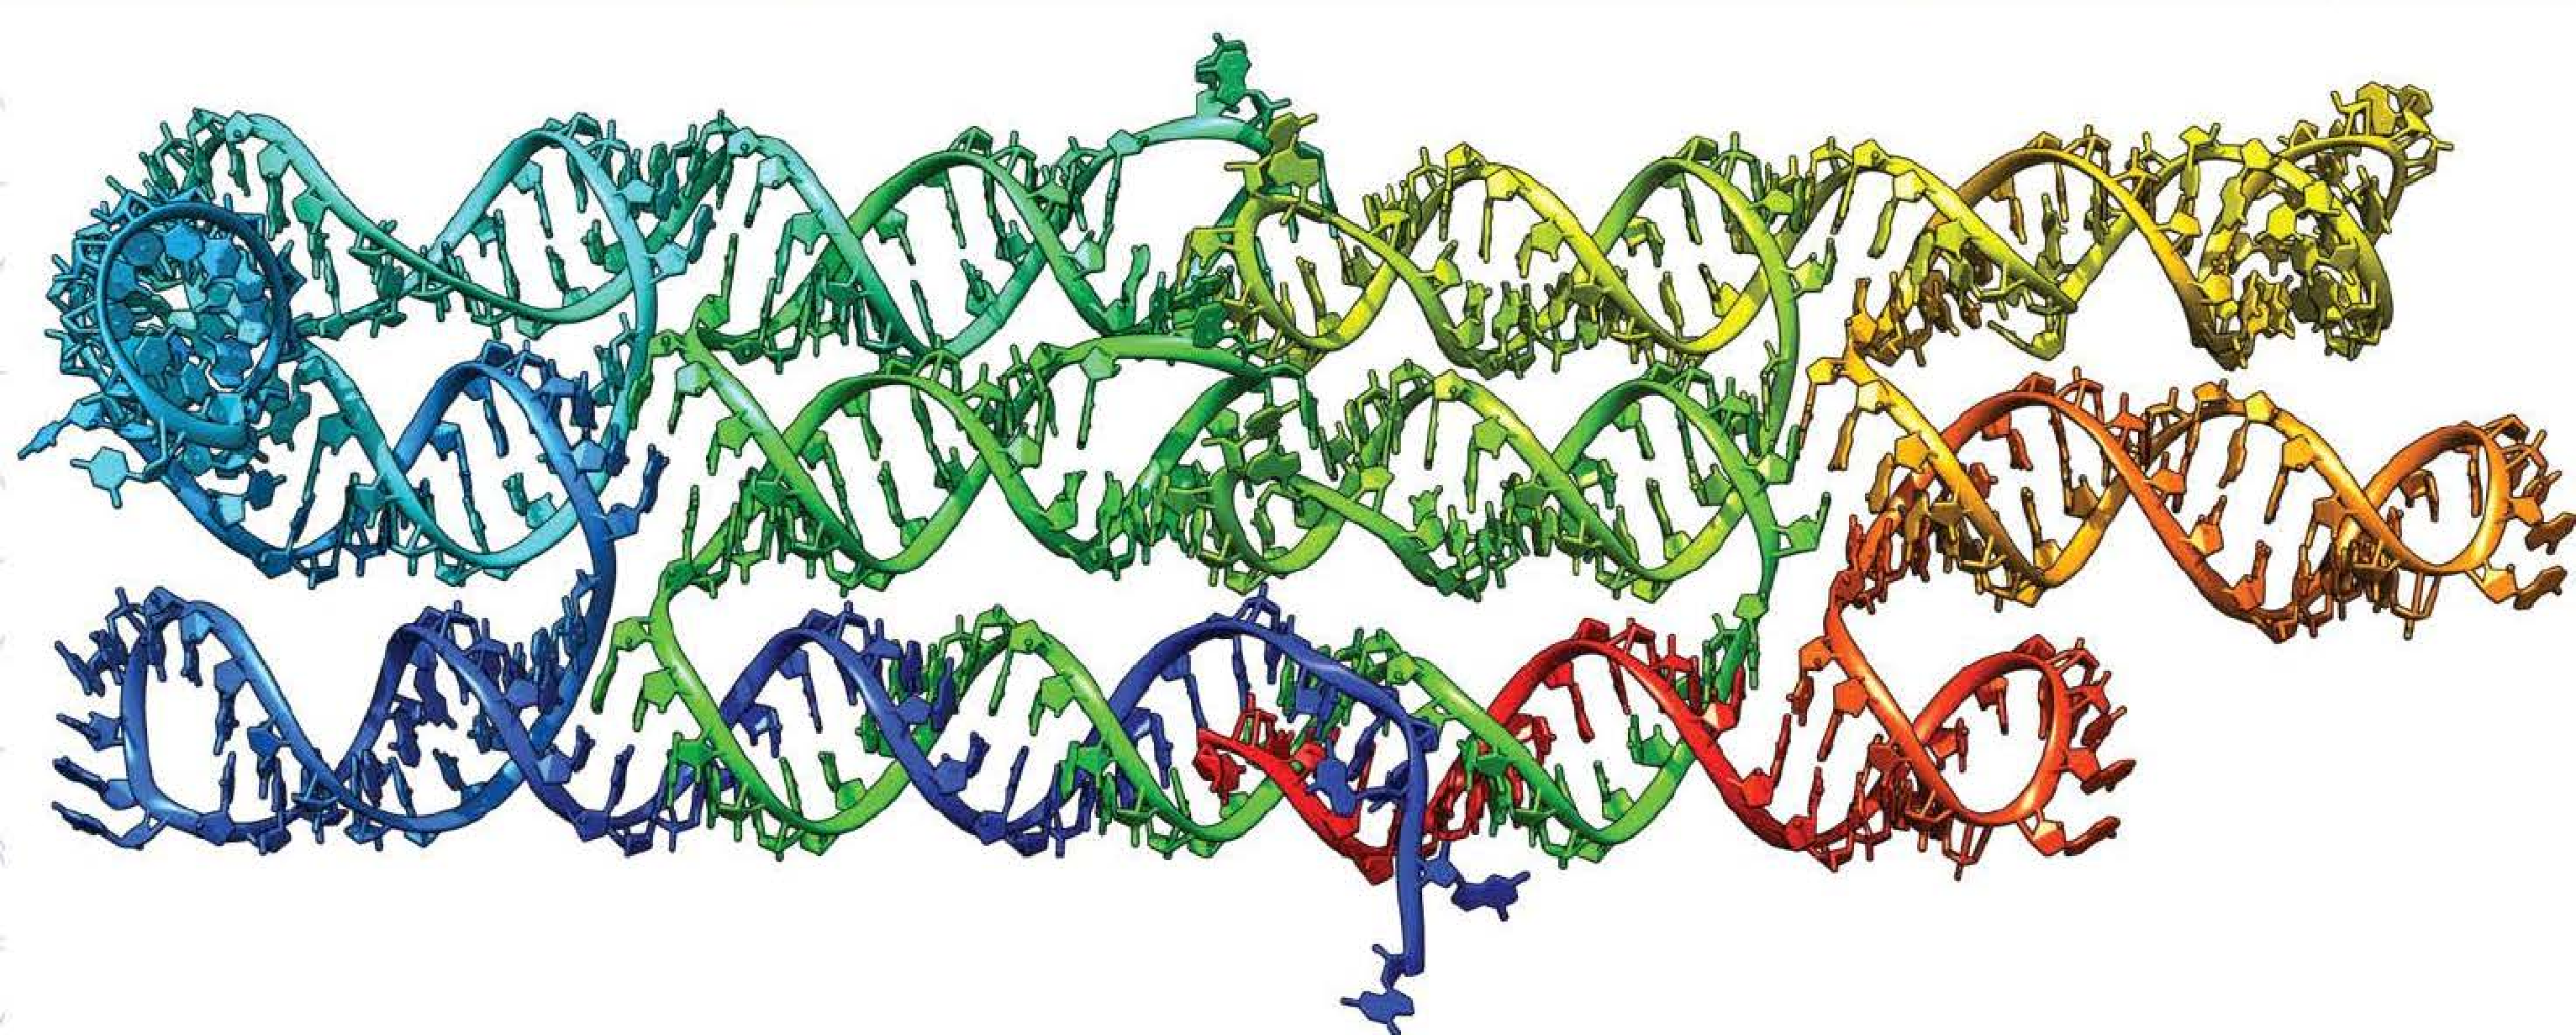
\includegraphics[width=0.6\linewidth]{rna_tile.pdf}
%\end{figure}
%\begin{minipage}{0.25\linewidth}
%\begin{tikzpicture}
%\centering
%\draw[-latex,thick] (-0.5, -1) -- node[above] {abstract} ++(0:1.5);
%\end{tikzpicture}
%\end{minipage}
%\begin{minipage}{0.6\linewidth}
%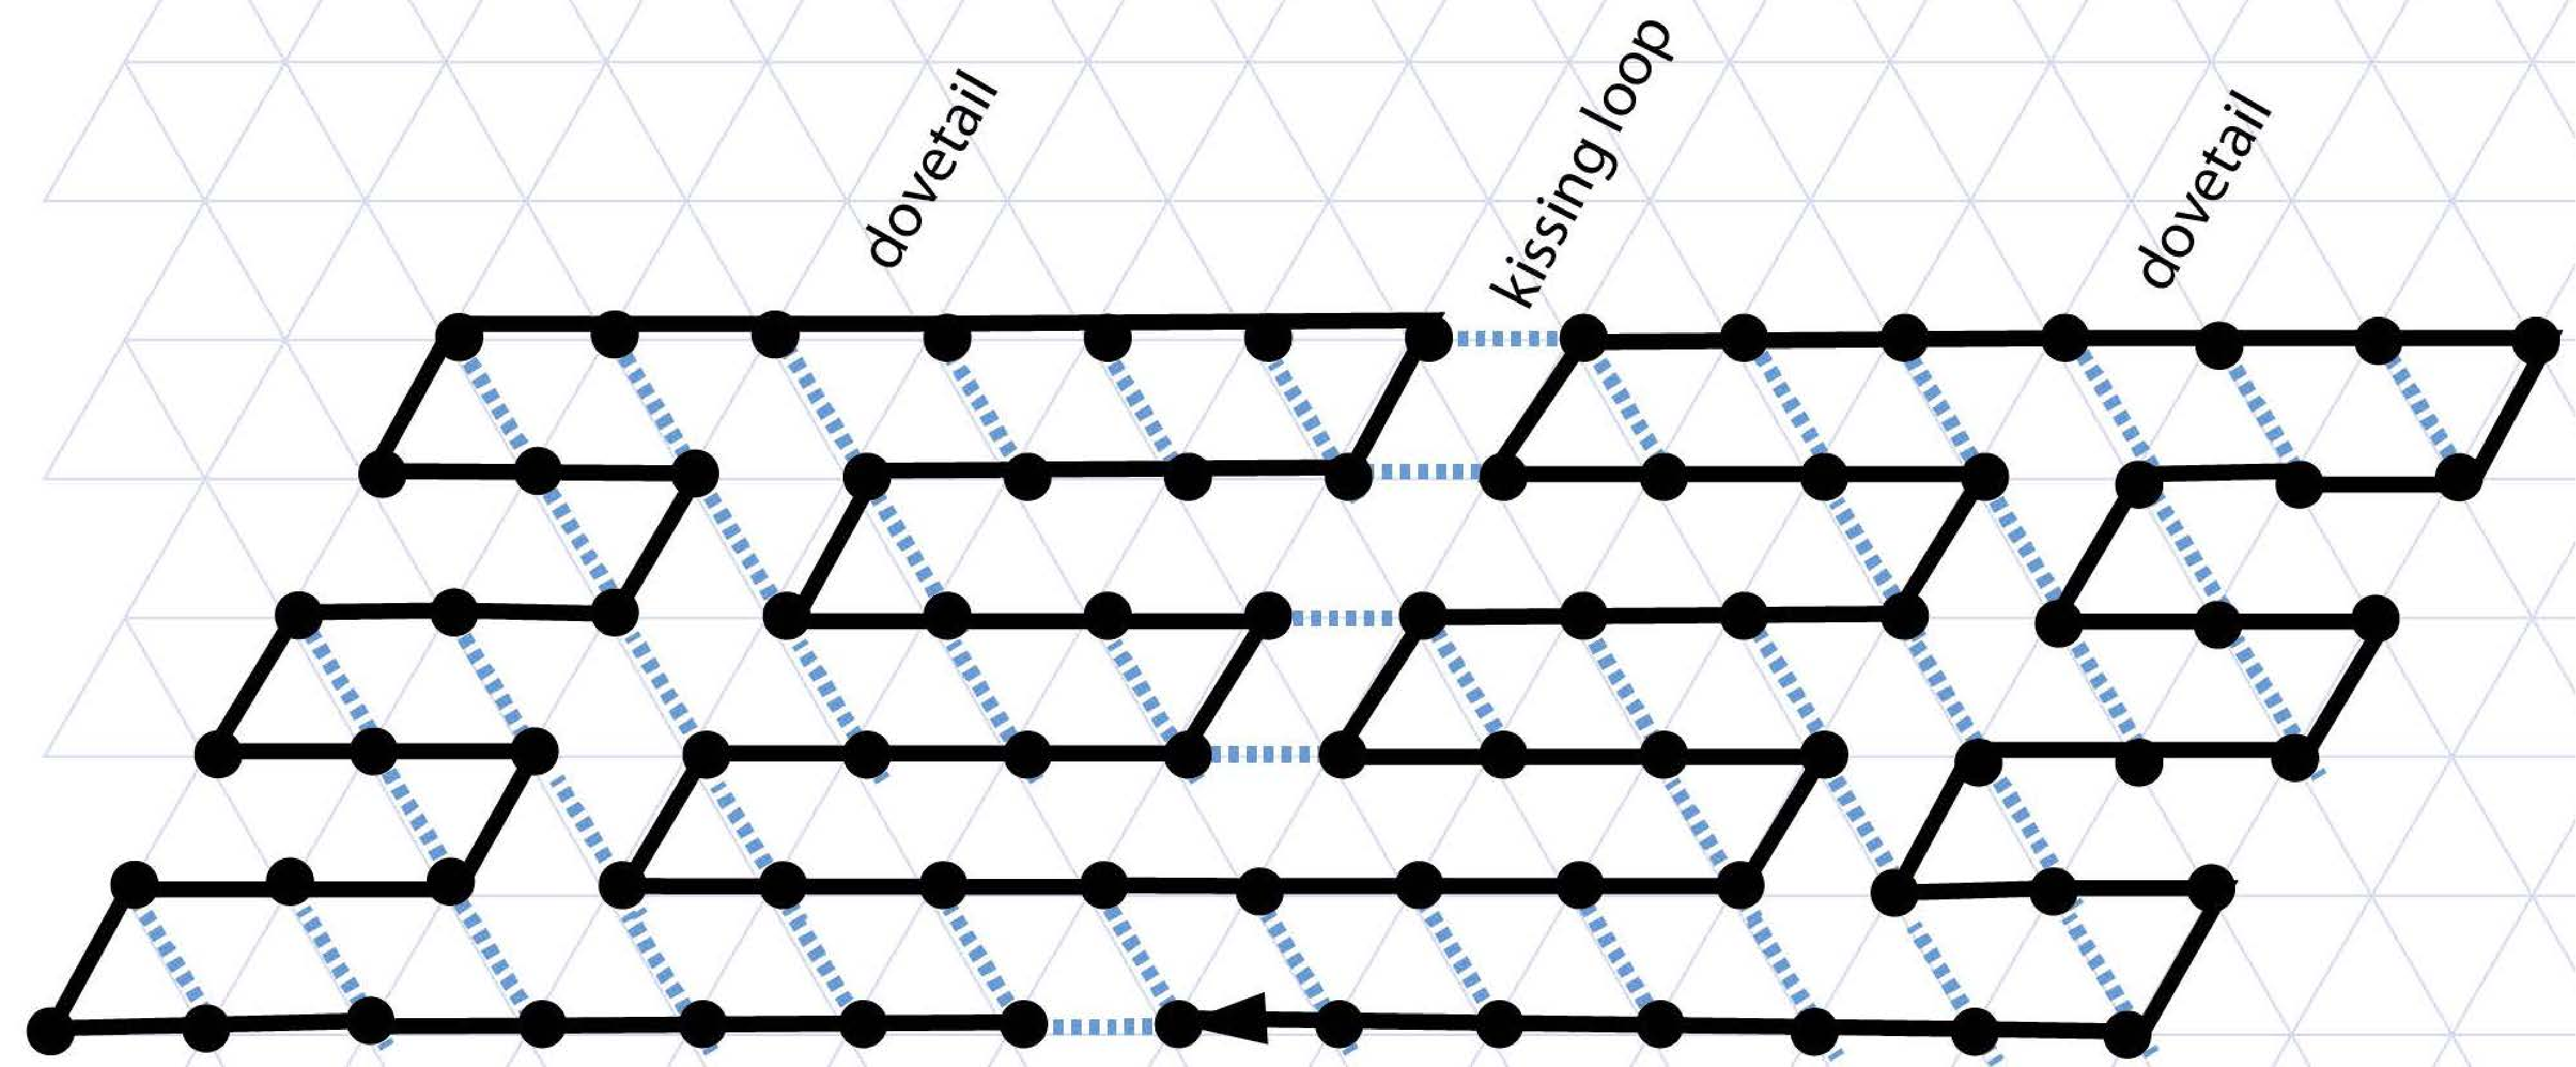
\includegraphics[width=\linewidth]{origami_oritatami.pdf}
%\end{minipage}
%
%
%\end{frame}
%%%%%%%%%%%%%%%%%%%%%%%%%%%%%%%%%%%%%%%%%%%%%%%%%%%%%%%%%%%%%%%%%%
\frame{
\frametitle{Oritatami System}
\framesubtitle{Definition}
\begin{center}
An oritatami system (OS) is a tuple $\Xi = (\Sigma, w, \mathcal{R}, \delta, \alpha)$, where
\begin{description}
\item[$\Sigma$] finite set of bead types
\item[$w \in \Sigma^*$] \emph{transcript}, a string to be folded
\item[$\mathcal{R} \in \Sigma \times \Sigma$] \emph{ruleset} to specify which types of beads can interact
\item[$\delta$] \emph{delay} (transcription rate) %, representing relative speed of transcription to conformational search
\item[$\alpha$] \emph{arity}, max \# of interactions per bead
%\item[$\sigma$] seed, initial structure
\end{description}
\end{center}
}%frame

%%%%%%%%%%%%%%%%%%%%%%%%%%%%%%%%%%%%%%%%%%%%%%%%%%%%%%%%
\frame{
\frametitle{Oritatami System}
\framesubtitle{Dynamics}

\begin{block}{Glider}
{\small Consider an OS with transcript $w = (b c a' a c' b')^*$, rule set $R = \{(a, a'), (b, b'), (c, c')\}$, delay $\delta = 3$, and the seed below colored in red.} 
\end{block}
\vspace*{3mm}

\begin{minipage}{0.4\linewidth}

{\scriptsize \begin{itemize}
\item Transcribe $w[1 .. \delta]$ at the 3'-end of the seed. 
\item for ($i = 0$, $i \le |w|$, $i = i+1$) \{ 
\begin{itemize}
{\scriptsize \item[1.] Fold $w[i .. i+\delta-1]$ in all geometrically-possible manners.}
{\scriptsize \item[2.] Stabilize $w[i]$ so as for $w[i .. i+\delta-1]$ to form as many bonds as possible.} 
{\scriptsize \item[3.] Transcribe $w[i+\delta]$ and $i = i+1$.\}} 

\end{itemize}
\end{itemize}}

\end{minipage}
\begin{minipage}{0.05\linewidth}
\ \\
\end{minipage}
\begin{minipage}{0.5\linewidth}

\begin{center}
\scalebox{1}{\begin{tikzpicture}

\foreach \x in {2, 3, 4, ..., 11} {
\foreach \y in {-2, 0} {
		\node[draw,circle,inner sep=0.5pt,fill] at (\x, \y * sin{60}) {};
		\node[draw,circle,inner sep=0.5pt,fill] at (\x+0.5, \y * sin{60} + sin{60}) {};
}
		\node[draw,circle,inner sep=0.5pt,fill] at (\x, 2 * sin{60}) {};
}

\foreach \x in {4} {
\draw[red,thick, -latex] (\x + 3,0)++(60:2)
-- ++(180:1) -- ++(180:1)-- ++(180:1) -- ++(180:1) -- ++(240:1) -- ++(300:1) -- ++(240:1) -- ++(0:1) node[below] {$a$} -- ++(60:1) node[below] {$b'$} -- ++(120:1);


\uncover<2>{\draw[teal,-latex] (\x,0)++(60:1) -- ++(0:1) node[above] {$b$} -- ++(0:1) node[below] {$c$} -- ++(0:1) node[above] {$a'$};}
\uncover<2->{\draw[dotted, very thick] (\x,0)++(0:1) -- ++(60:1);}
\uncover<3>{\draw[teal,-latex] (\x,0)++(60:1) -- ++(0:1) node[above] {$b$} -- ++(300:1) node[below] {$c$} -- ++ (0:1) node[below] {$a'$};
}
\uncover<4>{
\draw[teal,-latex] (\x,0)++(60:1) -- ++(0:1) node[above] {$b$} -- ++(300:1) node[below] {$c$} -- ++(240:1) node[below] {$a'$};
\draw[dotted, very thick] (\x,0)++(300:1) -- ++(0:1);
}
\uncover<5,8>{
\draw[teal,-latex] (\x+1,0)++(60:1) -- ++(300:1)node[below] {$c$} -- ++(240:1) node[below] {$a'$} -- ++(240:1) node[below] {$a$};
\draw[dotted, very thick] (\x,0)++(300:1) -- ++(0:1);
}
\uncover<5->{\draw[thick] (\x,0)++(60:1) -- ++(0:1) node[above] {$b$};}
\uncover<6>{
\draw[teal,-latex] (\x+1,0)++(60:1) -- ++(0:1) node[below] {$c$} -- ++(300:1) node[below] {$a'$} -- ++(240:1) node[below] {$a$};
}
\uncover<7>{
\draw[teal,-latex] (\x+1,0)++(60:1) -- ++(00:1) node[below] {$c$} -- ++(0:1) node[below] {$a'$} -- ++(0:1) node[below] {$a$};
}
\uncover<9->{\draw[thick] (\x+1,0)++(60:1) -- ++(300:1) node[below] {$c$};}
\uncover<9>{
\draw[teal,-latex] (\x+2,0) -- ++(240:1) node[below] {$a'$} -- ++(240:1) node[below] {$a$} -- ++(0:1) node[below] {$c'$};
\draw[dotted, very thick] (\x,0)++(300:1) -- ++(0:1);
}
\uncover<10->{
\draw[thick] (\x+2,0)--++(240:1) node[below] {$a'$};
\draw[dashed, very thick] (\x,0)++(300:1) -- ++(0:1);
}
\uncover<10>{\draw[teal,-latex] (\x+2,0)++(240:1) -- ++(240:1) node[below] {$a$} -- ++(0:1) node[below] {$c'$} -- ++(60:1) node[right] {$b'$};}
\uncover<11>{\draw[teal,-latex] (\x+2,0)++(240:1) -- ++(0:1) node[below] {$a$} -- ++(0:1) node[below] {$c'$} -- ++(60:1) node[right] {$b'$};}
\uncover<12>{
\draw[teal,-latex] (\x+2,0)++(240:1) -- ++(0:1) node[below] {$a$} -- ++(60:1) node[below] {$c'$} -- ++(120:1) node[above] {$b'$};
\draw[dotted, very thick] (\x+2,0)++(60:1) -- ++(180:1);
\draw[dotted, very thick] (\x,0)++(0:2) -- ++(0:1);
}
\uncover<13->{\draw[thick] (\x+2,0)++(240:1) -- ++(0:1) node[below] {$a$};}
\uncover<13>{
\draw[teal,-latex] (\x+3,0)++(240:1) -- ++(60:1) node[below] {$c'$} -- ++(120:1) node[above] {$b'$} -- ++(0:1) node[above] {$b$};
\draw[dotted, very thick] (\x+2,0)++(60:1) -- ++(180:1);
\draw[dotted, very thick] (\x,0)++(0:2) -- ++(0:1);
}
\uncover<14->{\draw[thick] (\x+3,0)++(240:1) -- ++(60:1)node[below] {$c'$};
\draw[dotted, very thick] (\x,0)++(0:2) -- ++(0:1);}
\uncover<14>{
\draw[teal,-latex] (\x+3,0) -- ++(120:1) node[above] {$b'$} -- ++(0:1) node[above] {$b$} -- ++(300:1) node[below] {$c$};
\draw[dotted, very thick] (\x+2,0)++(60:1) -- ++(180:1);
\draw[dotted, very thick] (\x,0)++(0:3) -- ++(0:1);
}
\uncover<15->{
\draw[thick] (\x+3,0) -- ++(120:1) node[above] {$b'$};
\draw[dashed, very thick] (\x+2,0)++(60:1) -- ++(180:1);
}
\uncover<15>{
\draw[teal,-latex] (\x+3,0)++(120:1) -- ++(0:1) node[above] {$b$} -- ++(300:1) node[below] {$c$} -- ++(240:1) node[below] {$a'$};
\draw[dotted, very thick] (\x+3,0)++(300:1) -- ++(180:1);
\draw[dotted, very thick] (\x,0)++(0:3) -- ++(0:1);
}
\uncover<16->{\draw[thick] (\x+3,0)++(120:1)-- ++(0:1) node[above] {$b$};
\draw[dotted, very thick] (\x,0)++(0:3) -- ++(0:1);}
\uncover<16>{
\draw[teal,-latex] (\x+3,0)++(60:1) -- ++(300:1)node[below] {$c$}  -- ++(240:1) node[below] {$a'$} -- ++(240:1) node[right] {$a$};
\draw[dotted, very thick] (\x+3,0)++(300:1) -- ++(180:1);
}

}%foreach \x

\end{tikzpicture}}
\end{center}

\end{minipage}




%The resulting conformations are called \emph{terminal}, which are the output of the system. 
}

%%%%%%%%%%%%%%%%%%%%%%%%%%%%%%%%%%%%%%%%%%%%%%%%%%%%%%%%
\frame{
\frametitle{Oritatami System}
\framesubtitle{Dynamics}

\begin{block}{Glider (Context-sensitive)}
{\small Consider an OS with transcript $w = (b c a' a c' b')^*$, rule set $R = \{(a, a'), (b, b'), (c, c')\}$, delay $\delta = 3$, and the seed below colored in red.} 
\end{block}
\vspace*{3mm}

\begin{minipage}{0.4\linewidth}

{\scriptsize \begin{itemize}
\item Transcribe $w[1 .. \delta]$ at the 3'-end of the seed. 
\item for ($i = 0$, $i \le |w|$, $i = i+1$) \{ 
\begin{itemize}
{\scriptsize \item[1.] Fold $w[i .. i+\delta-1]$ in all geometrically-possible manners.}
{\scriptsize \item[2.] Stabilize $w[i]$ so as for $w[i .. i+\delta-1]$ to form as many bonds as possible.} 
{\scriptsize \item[3.] Transcribe $w[i+\delta]$ and $i = i+1$.\}} 

\end{itemize}
\end{itemize}}

\end{minipage}
\begin{minipage}{0.05\linewidth}
\ \\
\end{minipage}
\begin{minipage}{0.5\linewidth}

\begin{center}
\scalebox{1}{\begin{tikzpicture}

\foreach \x in {2, 3, 4, ..., 11} {
\foreach \y in {-2, 0} {
		\node[draw,circle,inner sep=0.5pt,fill] at (\x, \y * sin{60}) {};
		\node[draw,circle,inner sep=0.5pt,fill] at (\x+0.5, \y * sin{60} + sin{60}) {};
}
		\node[draw,circle,inner sep=0.5pt,fill] at (\x, 2 * sin{60}) {};
}

\foreach \x in {4} {
\draw[red,thick, -latex] (\x + 3,0)++(60:2) node[below] {$a$}
-- ++(180:1) node[below] {$a$} -- ++(180:1)-- ++(180:1) -- ++(180:1) -- ++(240:1) -- ++(300:1) -- ++(240:1) -- ++(0:1) node[below] {$a$} -- ++(60:1) node[below] {$b'$} -- ++(120:1);

\uncover<2->{\draw[dotted, very thick] (\x,0)++(0:1) -- ++(60:1);}
\uncover<2>{
\draw[teal,-latex] (\x,0)++(60:1) -- ++(0:1) node[above] {$b$} -- ++(300:1) node[below] {$c$} -- ++(240:1) node[below] {$a'$};
\draw[dotted, very thick] (\x,0)++(300:1) -- ++(0:1);
}
\uncover<3>{\draw[teal,-latex] (\x,0)++(60:1) -- ++(0:1) node[above] {$b$} -- ++(300:1) node[below] {$c$} -- ++ (300:1) node[below] {$a'$};}
\uncover<4>{
\draw[teal,-latex] (\x,0)++(60:1) -- ++(0:1) node[above] {$b$} -- ++(0:1) node[below] {$c$}-- ++(0:1) node[below] {$a'$};
\draw[dotted, very thick] (\x+3,0)++(60:2) -- ++(240:1);
\draw[dotted, very thick] (\x+2,0)++(60:2) -- ++(300:1);
}
\uncover<5>{
\draw[teal,-latex] (\x+1,0)++(60:1) -- ++(300:1) node[below] {$c$} -- ++(240:1) node[below] {$a'$} -- ++(240:1) node[below] {$a$};
\draw[dotted, very thick] (\x,0)++(300:1) -- ++(0:1);
}
\uncover<5->{\draw[thick] (\x,0)++(60:1) -- ++(0:1) node[above] {$b$};}
\uncover<6>{
\draw[teal,-latex] (\x+1,0)++(60:1) -- ++(0:1) node[below] {$c$} -- ++(300:1) node[below] {$a'$} -- ++(240:1) node[below] {$a$};
}
\uncover<7>{
\draw[teal,-latex] (\x+1,0)++(60:1)  -- ++(0:1)node[below] {$c$} -- ++(0:1) node[below] {$a'$} -- ++(0:1) node[below] {$a$};
\draw[dotted, very thick] (\x+3,0)++(60:2) -- ++(240:1);
\draw[dotted, very thick] (\x+2,0)++(60:2) -- ++(300:1);
}
\uncover<8->{\draw[thick] (\x+1,0)++(60:1) -- ++(0:1) node[below] {$c$};}
\uncover<8>{
\draw[teal,-latex] (\x+2,0)++(60:1) -- ++(240:1) node[below] {$a'$} -- ++(240:1) node[below] {$a$}-- ++(240:1)node[below] {$c$};
}
\uncover<9>{
\draw[teal,-latex] (\x+2,0)++(60:1) -- ++(0:1) node[below] {$a'$} -- ++(240:1) node[below] {$a$}  -- ++(240:1)node[below] {$c`$};
\draw[dotted, very thick] (\x+3,0)++(60:2) -- ++(240:1);
\draw[dotted, very thick] (\x+2,0)++(60:2) -- ++(300:1);
}
\uncover<10->{
\draw[thick] (\x+2,0)++(60:1) -- ++(0:1) node[below] {$a'$};
\draw[dotted, very thick] (\x+3,0)++(60:2) -- ++(240:1);
\draw[dotted, very thick] (\x+2,0)++(60:2) -- ++(300:1);
}

\uncover<10>{\draw[teal,-latex] (\x+3,0)++(60:1) -- ++(240:1) node[below] {$a$} -- ++(240:1) node[below] {$c'$} -- ++(120:1) node[above] {$b'$};
\draw[dotted, very thick] (\x+1,0)++(60:1) -- ++(300:1);
}
\uncover<11>{\draw[teal,-latex] (\x+3,0)++(60:1) -- ++(300:1) node[below] {$a$} -- ++(180:1) node[below] {$c'$} -- ++(180:1) node[above] {$b'$};
\draw[dotted, very thick] (\x+1,0)++(60:1) -- ++(300:1);
\draw[dotted, very thick] (\x+2,0)++(60:1) -- ++(300:1);
}
\uncover<12>{\draw[teal,-latex] (\x+3,0)++(60:1) -- ++(0:1) node[below] {$a$} -- ++(240:1) node[below] {$c'$} -- ++(180:1) node[above] {$b'$};
}

\uncover<13->{
\draw[thick] (\x+3,0)++(60:1) -- ++(300:1) node[below] {$a$};
}
\uncover<13>{\draw[teal,-latex] (\x+3,0)++(0:1) -- ++(180:1)node[below] {$c'$} -- ++(180:1)  node[above] {$b'$} -- ++(240:1) node[above] {$b$};
\draw[dotted, very thick] (\x+1,0)++(60:1) -- ++(300:1);
\draw[dotted, very thick] (\x+2,0)++(60:1) -- ++(300:1);
\draw[dotted, very thick] (\x,0)++(0:1) -- ++(300:1);
}
\uncover<14->{
\draw[thick] (\x+3,0)++(0:1) -- ++(180:1) node[below] {$c'$};
\draw[dotted, very thick] (\x+2,0)++(60:1) -- ++(300:1);
}
\uncover<14>{\draw[teal,-latex] (\x+2,0)++(0:1) -- ++(180:1)node[above] {$b'$} -- ++(240:1) node[above] {$b$} -- ++(0:1)node[below] {$c$};
\draw[dotted, very thick] (\x+1,0)++(60:1) -- ++(300:1);
\draw[dotted, very thick] (\x+2,0)++(60:1) -- ++(300:1);
\draw[dotted, very thick] (\x,0)++(0:1) -- ++(300:1);
\draw[dotted, very thick] (\x+2,0)++(0:1) -- ++(240:1);
}
\uncover<15->{
\draw[thick] (\x+2,0)++(0:1) -- ++(180:1) node[above] {$b'$};
\draw[dotted, very thick] (\x+1,0)++(60:1) -- ++(300:1);
}
\uncover<15>{\draw[teal,-latex] (\x+1,0)++(0:1) -- ++(240:1)node[above] {$b$} -- ++(0:1) node[below] {$c$} -- ++(0:1)node[above] {$a'$};
\draw[dotted, very thick] (\x,0)++(0:1) -- ++(300:1);
\draw[dotted, very thick] (\x+2,0)++(0:1) -- ++(240:1);
\draw[dotted, very thick] (\x+3,0)++(0:1) -- ++(240:1);
}

}%foreach \x

\end{tikzpicture}}
\end{center}

\end{minipage}
%The resulting conformations are called \emph{terminal}, which are the output of the system. 
}

%%%%%%%%%%%%%%%%%%%%%%%%%%%%%%%%%%%%%%%%%%%%%%%%%%%%%%%%%%%%%%%%%%

\begin{frame}\frametitle{\it{Module} \scriptsize{\cite{GeMeScSe2016}}}

\begin{figure}
\begin{center}
\scalebox{1.2}{
\begin{tikzpicture}
\draw[thick] (0,0)-- ++(0:1.5)-- ++(120:1) -- ++(180:1.5)-- ++(300:1); 
\draw[thick, -latex] (-0.25,0) ++ (120:1) ++ (0:1.25) ++(90:0.25) node [above] {input} -- ++(270:0.5);
\draw[thick, -latex] (1.5,0) ++ (120:0.5) ++(0:0.25) node [right] {input} -- ++(180:0.5);
\draw[thick, -latex] (0.5,0.25) -- ++ (270:0.5) node [below] {output};
\draw[thick, -latex] (0,0) ++ (120:0.5) ++(0:0.25) -- ++(180:0.5) node [left] {output};
\end{tikzpicture}
}
\end{center}
\end{figure}
\only<1>{
\begin{figure}[htb]
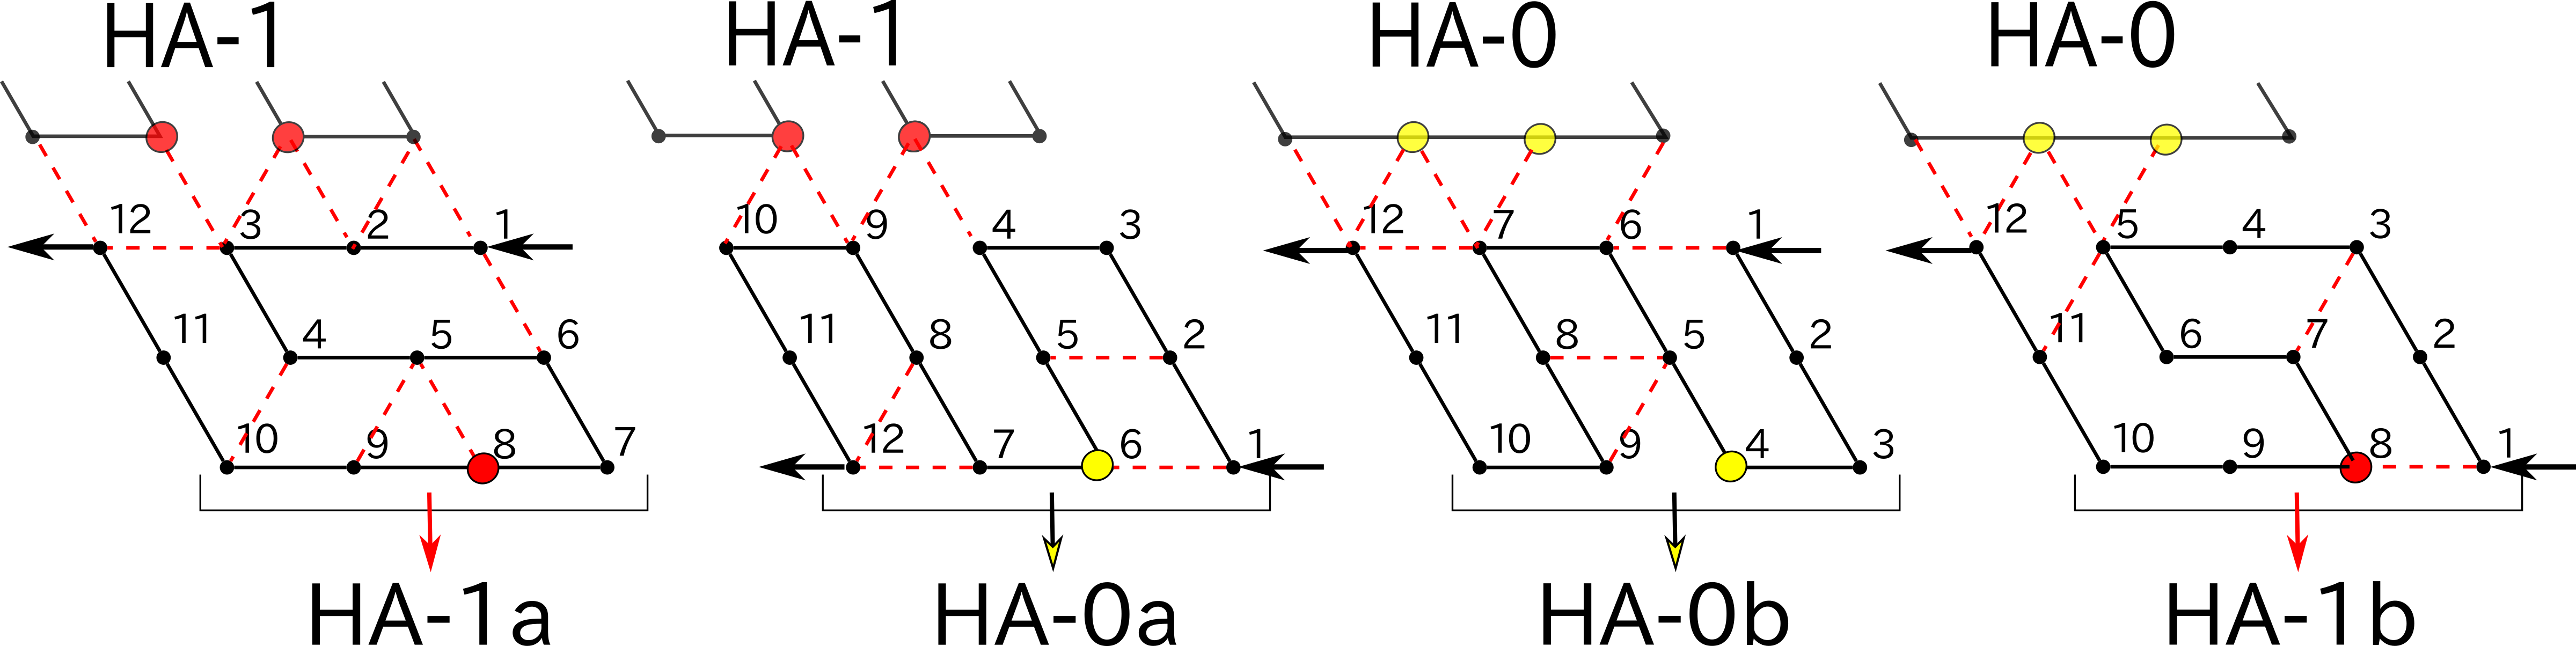
\includegraphics[width = \linewidth]{counter_zig.png}
\caption{Four bricks of Half Adder \it{module}}
\end{figure}
}
\only<2>{
\vspace{2zh}
\begin{figure}[H]
  \begin{tabular}{c}
  \begin{minipage}{0.23\hsize}
  \centering
\scalebox{0.9}{
  \begin{tikzpicture}
\draw[thick] (0,0)-- ++(0:1.5)-- ++(120:1) -- ++(180:1.5)-- ++(300:1); 
\draw[thick, -latex] (-0.25,0) ++ (120:1) ++ (0:1.25) ++(90:0.25) node [above] {1} -- ++(270:0.5);
\draw[thick, -latex] (1.5,0) ++ (120:0.5) ++(0:0.25) node [right] {0} -- ++(180:0.5);
\draw[thick, -latex] (0.5,0.25) -- ++ (270:0.5) node [below] {1};
\draw[thick, -latex] (0,0) ++ (120:0.5) ++(0:0.25) -- ++(180:0.5) node [left] {0};
\end{tikzpicture}
  }
  \end{minipage}

\begin{minipage}{0.23\hsize}
  \centering
\scalebox{0.9}{
\begin{tikzpicture}
\draw[thick] (0,0)-- ++(0:1.5)-- ++(120:1) -- ++(180:1.5)-- ++(300:1); 
\draw[thick, -latex] (-0.25,0) ++ (120:1) ++ (0:1.25) ++(90:0.25) node [above] {1} -- ++(270:0.5);
\draw[thick, -latex] (1.5,0) ++ (120:0.5) ++(0:0.25) node [right] {1} -- ++(180:0.5);
\draw[thick, -latex] (0.5,0.25) -- ++ (270:0.5) node [below] {0};
\draw[thick, -latex] (0,0) ++ (120:0.5) ++(0:0.25) -- ++(180:0.5) node [left] {1};
\end{tikzpicture}
 }
  \end{minipage}

\begin{minipage}{0.23\hsize}
  \centering
\scalebox{0.9}{  
\begin{tikzpicture}
\draw[thick] (0,0)-- ++(0:1.5)-- ++(120:1) -- ++(180:1.5)-- ++(300:1); 
\draw[thick, -latex] (-0.25,0) ++ (120:1) ++ (0:1.25) ++(90:0.25) node [above] {0} -- ++(270:0.5);
\draw[thick, -latex] (1.5,0) ++ (120:0.5) ++(0:0.25) node [right] {0} -- ++(180:0.5);
\draw[thick, -latex] (0.5,0.25) -- ++ (270:0.5) node [below] {0};
\draw[thick, -latex] (0,0) ++ (120:0.5) ++(0:0.25) -- ++(180:0.5) node [left] {0};
\end{tikzpicture}
  }
  \end{minipage}


\begin{minipage}{0.23\hsize}
  \centering
\scalebox{0.9}{
  \begin{tikzpicture}
\draw[thick] (0,0)-- ++(0:1.5)-- ++(120:1) -- ++(180:1.5)-- ++(300:1); 
\draw[thick, -latex] (-0.25,0) ++ (120:1) ++ (0:1.25) ++(90:0.25) node [above] {0} -- ++(270:0.5);
\draw[thick, -latex] (1.5,0) ++ (120:0.5) ++(0:0.25) node [right] {1} -- ++(180:0.5);
\draw[thick, -latex] (0.5,0.25) -- ++ (270:0.5) node [below] {1};
\draw[thick, -latex] (0,0) ++ (120:0.5) ++(0:0.25) -- ++(180:0.5) node [left] {0};
\end{tikzpicture}
 }
  \end{minipage}
  \end{tabular}
 \caption{Four bricks of Half Adder \it{module}}
\end{figure} 
}
\end{frame}

%%%%%%%%%%%%%%%%%%%%%%%%%%%%%%%%%%%%%%%%%%%%%%%%%%%%%%%%%%%%%%%%%%%%%%

%\begin{frame}\frametitle{\it{Module}}
%\begin{figure}
%
%\begin{center}
%\scalebox{1.2}{
%\begin{tikzpicture}
%\draw[thick] (0,0)-- ++(0:1.5)-- ++(120:1) -- ++(180:1.5)-- ++(300:1); 
%\draw[thick, -latex] (-0.25,0) ++ (120:1) ++ (0:1.25) ++(90:0.25) node [above] {input} -- ++(270:0.5);
%\draw[thick, -latex] (1.5,0) ++ (120:0.5) ++(0:0.25) node [right] {input} -- ++(180:0.5);
%\draw[thick, -latex] (0.5,0.25) -- ++ (270:0.5) node [below] {output};
%\draw[thick, -latex] (0,0) ++ (120:0.5) ++(0:0.25) -- ++(180:0.5) node [left] {output};
%\end{tikzpicture}
%}
%\end{center}
%\end{figure}
%\vspace{2zh}
%% %%
%\begin{figure}[H]
%  \begin{tabular}{c}
%  \begin{minipage}{0.23\hsize}
%  \centering
%\scalebox{0.9}{
%  \begin{tikzpicture}
%\draw[thick] (0,0)-- ++(0:1.5)-- ++(120:1) -- ++(180:1.5)-- ++(300:1); 
%\draw[thick, -latex] (-0.25,0) ++ (120:1) ++ (0:1.25) ++(90:0.25) node [above] {1} -- ++(270:0.5);
%\draw[thick, -latex] (1.5,0) ++ (120:0.5) ++(0:0.25) node [right] {0} -- ++(180:0.5);
%\draw[thick, -latex] (0.5,0.25) -- ++ (270:0.5) node [below] {1};
%\draw[thick, -latex] (0,0) ++ (120:0.5) ++(0:0.25) -- ++(180:0.5) node [left] {0};
%\end{tikzpicture}
%  }
%  \end{minipage}
%
%\begin{minipage}{0.23\hsize}
%  \centering
%\scalebox{0.9}{
%\begin{tikzpicture}
%\draw[thick] (0,0)-- ++(0:1.5)-- ++(120:1) -- ++(180:1.5)-- ++(300:1); 
%\draw[thick, -latex] (-0.25,0) ++ (120:1) ++ (0:1.25) ++(90:0.25) node [above] {1} -- ++(270:0.5);
%\draw[thick, -latex] (1.5,0) ++ (120:0.5) ++(0:0.25) node [right] {1} -- ++(180:0.5);
%\draw[thick, -latex] (0.5,0.25) -- ++ (270:0.5) node [below] {0};
%\draw[thick, -latex] (0,0) ++ (120:0.5) ++(0:0.25) -- ++(180:0.5) node [left] {1};
%\end{tikzpicture}
% }
%  \end{minipage}
%
%\begin{minipage}{0.23\hsize}
%  \centering
%\scalebox{0.9}{  
%\begin{tikzpicture}
%\draw[thick] (0,0)-- ++(0:1.5)-- ++(120:1) -- ++(180:1.5)-- ++(300:1); 
%\draw[thick, -latex] (-0.25,0) ++ (120:1) ++ (0:1.25) ++(90:0.25) node [above] {0} -- ++(270:0.5);
%\draw[thick, -latex] (1.5,0) ++ (120:0.5) ++(0:0.25) node [right] {0} -- ++(180:0.5);
%\draw[thick, -latex] (0.5,0.25) -- ++ (270:0.5) node [below] {0};
%\draw[thick, -latex] (0,0) ++ (120:0.5) ++(0:0.25) -- ++(180:0.5) node [left] {0};
%\end{tikzpicture}
%  }
%  \end{minipage}
%
%
%\begin{minipage}{0.23\hsize}
%  \centering
%\scalebox{0.9}{
%  \begin{tikzpicture}
%\draw[thick] (0,0)-- ++(0:1.5)-- ++(120:1) -- ++(180:1.5)-- ++(300:1); 
%\draw[thick, -latex] (-0.25,0) ++ (120:1) ++ (0:1.25) ++(90:0.25) node [above] {0} -- ++(270:0.5);
%\draw[thick, -latex] (1.5,0) ++ (120:0.5) ++(0:0.25) node [right] {1} -- ++(180:0.5);
%\draw[thick, -latex] (0.5,0.25) -- ++ (270:0.5) node [below] {1};
%\draw[thick, -latex] (0,0) ++ (120:0.5) ++(0:0.25) -- ++(180:0.5) node [left] {0};
%\end{tikzpicture}
% }
%  \end{minipage}
%  \end{tabular}
% \caption{Four bricks of Half Adder \it{module}}
%\end{figure} 
%
%\end{frame}
%
%
%
%%%%%%%%%%%%%%%%%%%%%%%%%%%%%%%%%%%%%%%%%%%%%%%%%%%%%%%%%%%%%%%%%%

\begin{frame}\frametitle{\it{Module} \scriptsize{\cite{GeMeScSe2016}}}
\begin{center}
\scalebox{0.85}{
\begin{tikzpicture}
\foreach \x in {12}{
\draw[thick,-latex,red](3,10)-- ++(0:9)-- ++(0:0.5)-- ++(300:1.5)-- ++(180:0.5);
\draw[thick,blue](10,10)-- ++(0:1) node [above] {\LARGE{HA-0}}-- ++(0:1);
\draw[thick,blue](5,10)-- ++(0:1) node [above] {\LARGE{HA-0}}-- ++(0:1);

\uncover<2->{\draw[thick,orange] (\x,10)++(300:1.5)-- ++(180:1.2) node [above, orange] {\LARGE{HA-1b}} -- ++(180:0.8)-- ++(120:1)-- ++(0:2)-- ++(300:1);
\draw[thick,orange,-latex] (\x-2,10)++(300:0.5)-- ++(180:0.5);
}

\uncover<3->{\draw[thick] (\x -2.5,10)++(300:1.5)-- ++(180:2)-- ++(120:1)-- ++(0:2)-- ++(300:1);
\draw[thick,-latex] (\x-4.5,10)++(300:0.5)-- ++(180:0.5);
}

\uncover<4->{\draw[thick,orange] (\x -5,10)++(300:1.5)-- ++(180:1.2) node [above, orange] {\LARGE{HA-0b}} -- ++(180:0.8)-- ++(120:1)-- ++(0:2)-- ++(300:1);
\draw[thick,orange,-latex] (\x-7,10)++(300:0.5)-- ++(180:0.5);
}

\uncover<5->{\draw[thick] (\x -7.5,10) ++(300:1.5)-- ++(120 :1)-- ++(180:1)-- ++(300:2.5)-- ++(0:1)-- ++(120:1.5);
\draw[thick,-latex] (\x-7.5,10)++(300:2)-- ++(0:0.5);
}

\uncover<6->{\draw[thick,orange] (\x -5,10)++(300:3)-- ++(180:1.2) node [above, orange] {\LARGE{HA-0}} -- ++(180:0.8)-- ++(120:1)-- ++(0:2)-- ++(300:1);
\draw[thick,orange,-latex] (\x-5,10)++(300:2)-- ++(0:0.5);
}

\uncover<7->{\draw[thick] (\x -2.5,10)++(300:3)-- ++(180:2)-- ++(120:1)-- ++(0:2)-- ++(300:1);
\draw[thick,-latex] (\x-2.5,10)++(300:2)-- ++(0:0.5);
}

\uncover<8->{\draw[thick,orange] (\x,10)++(300:3)-- ++(180:1.2) node [above , orange] {\LARGE{HA-1}} -- ++(180:0.8)-- ++(120:1)-- ++(0:2)-- ++(300:1);
\draw[thick,orange,-latex] (\x,10)++(300:2)-- ++(0:0.5);
}

\uncover<9->{\draw[thick] (\x +1.5,10) ++(300:3)-- ++(120 :1)-- ++(180:1)-- ++(300:2.5)-- ++(0:1)-- ++(120:1.5);
\draw[thick,-latex] (\x+0.5,10)++(300:4.5)-- ++(180:0.5);
}

\uncover<10->{\draw[thick,orange] (\x,10)++(300:4.5)-- ++(180:1.2) node [above, orange] {\LARGE{HA-0a}} -- ++(180:0.8)-- ++(120:1)-- ++(0:2)-- ++(300:1);
\draw[thick,orange,-latex] (\x-2,10)++(300:4.5)-- ++(180:0.5);
}
\uncover<11->{\draw[thick] (\x -2.5,10)++(300:4.5)-- ++(180:2)-- ++(120:1)-- ++(0:2)-- ++(300:1);
\draw[thick,-latex] (\x-4.5,10)++(300:4.5)-- ++(180:0.5);
}
\uncover<12->{\draw[thick,orange] (\x-5,10)++(300:4.5)-- ++(180:1.2) node [above, orange] {\LARGE{HA-1b}} -- ++(180:0.8)-- ++(120:1)-- ++(0:2)-- ++(300:1);
\draw[thick,orange,-latex] (\x-7,10)++(300:3.5)-- ++(180:0.5);
}
}
\end{tikzpicture}
}
\end{center}
\begin{figure}[htb]
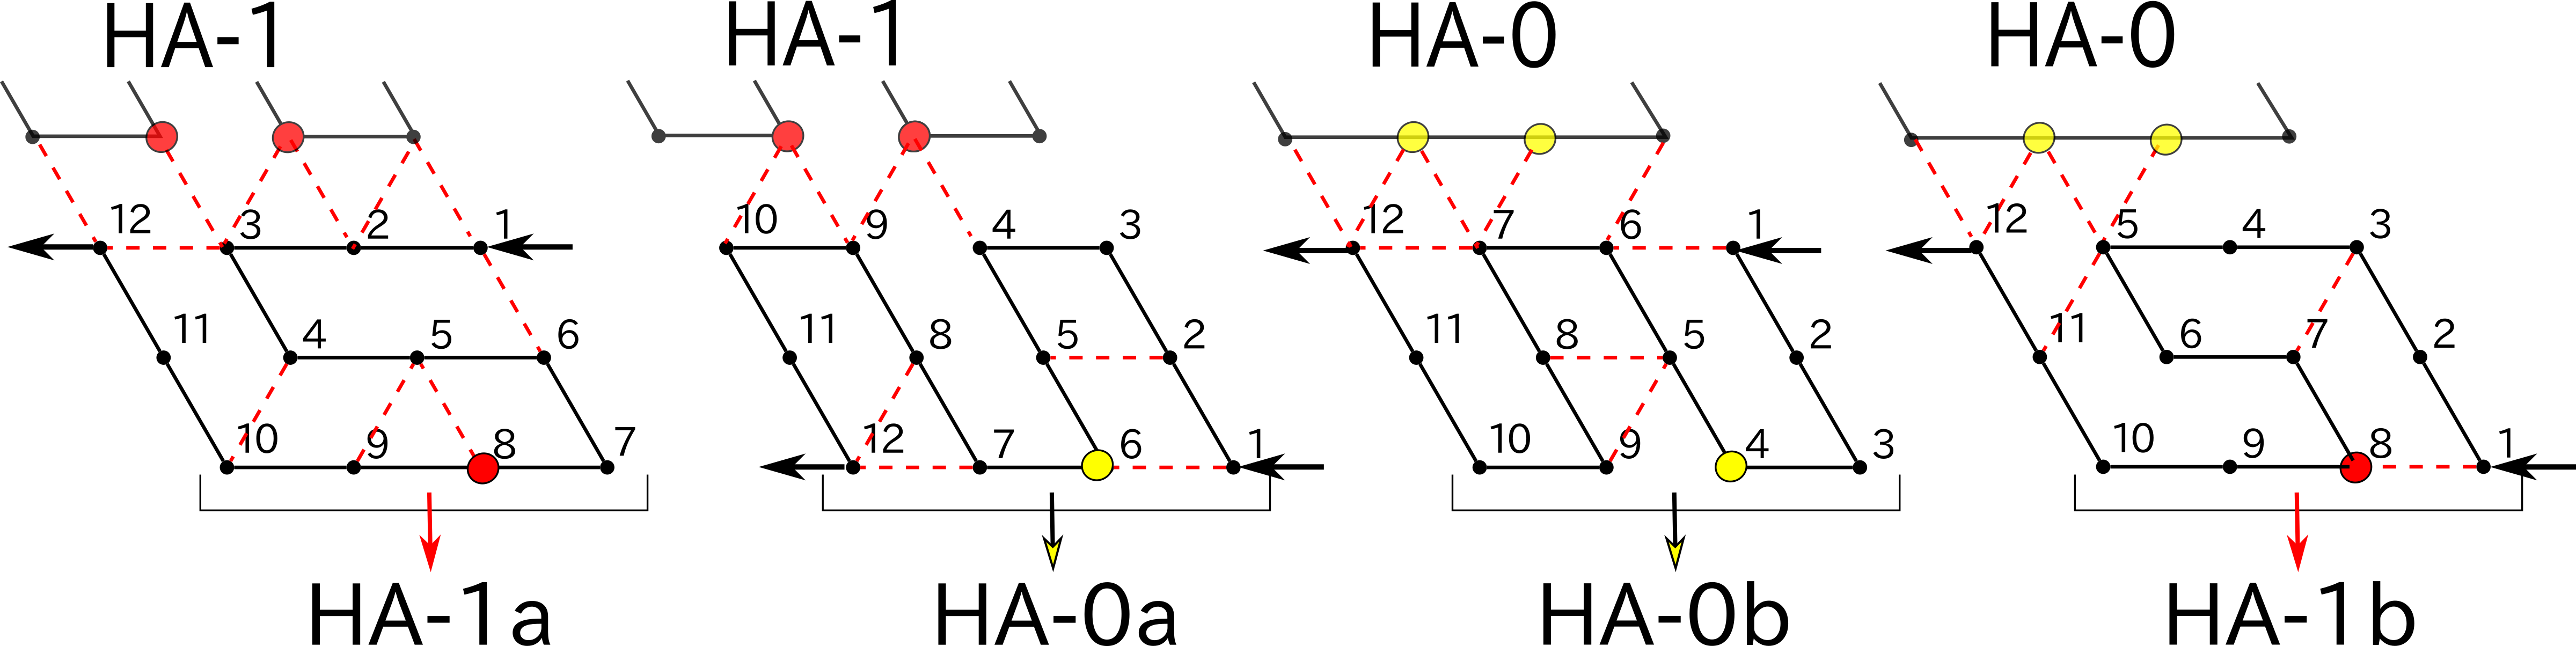
\includegraphics[width = 0.7\linewidth]{counter_zig.png}
\end{figure}
\end{frame}
%%%%%%%%%%%%%%%%%%%%%%%%%%%%%%%%%%%%%%%%%%%%%%%%%%%%%%%%%%%%%%%%%%
\begin{frame}\frametitle{\it{Module} \scriptsize{\cite{GeMeScSe2016}}}
\begin{figure}
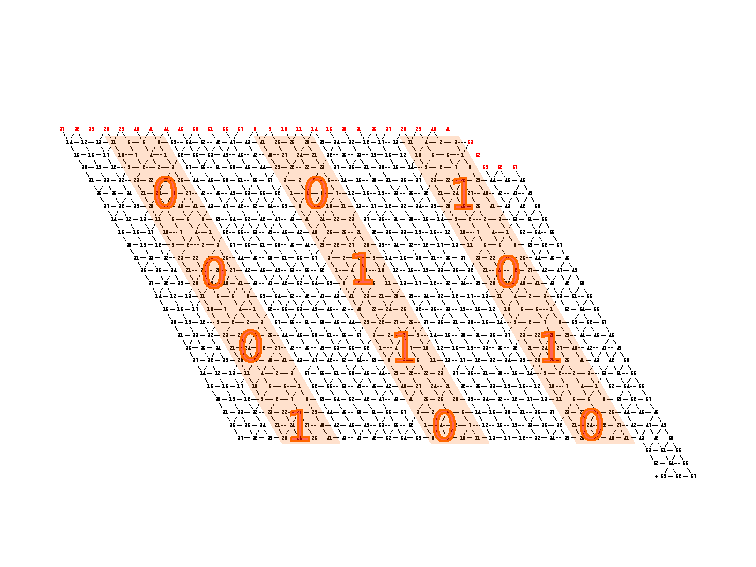
\includegraphics[width=\linewidth]{sample_counter.pdf}
\caption{Oritatami Counter}
\end{figure}
\end{frame}
%%%%%%%%%%%%%%%%%%%%%%%%%%%%%%%%%%%%%%%%%%%%%%%%%%%%%%%%%%%%%%%%%%
\section{Main results}

\begin{frame}\frametitle{Implementation}

\begin{itemize}
\item We design an oritatami system that self-assembles an $n$-bit fraction of the Heighway dragon.
\end{itemize}
\begin{figure}[H]
  	\centering
	\href{run:Dragon.mp4}{
	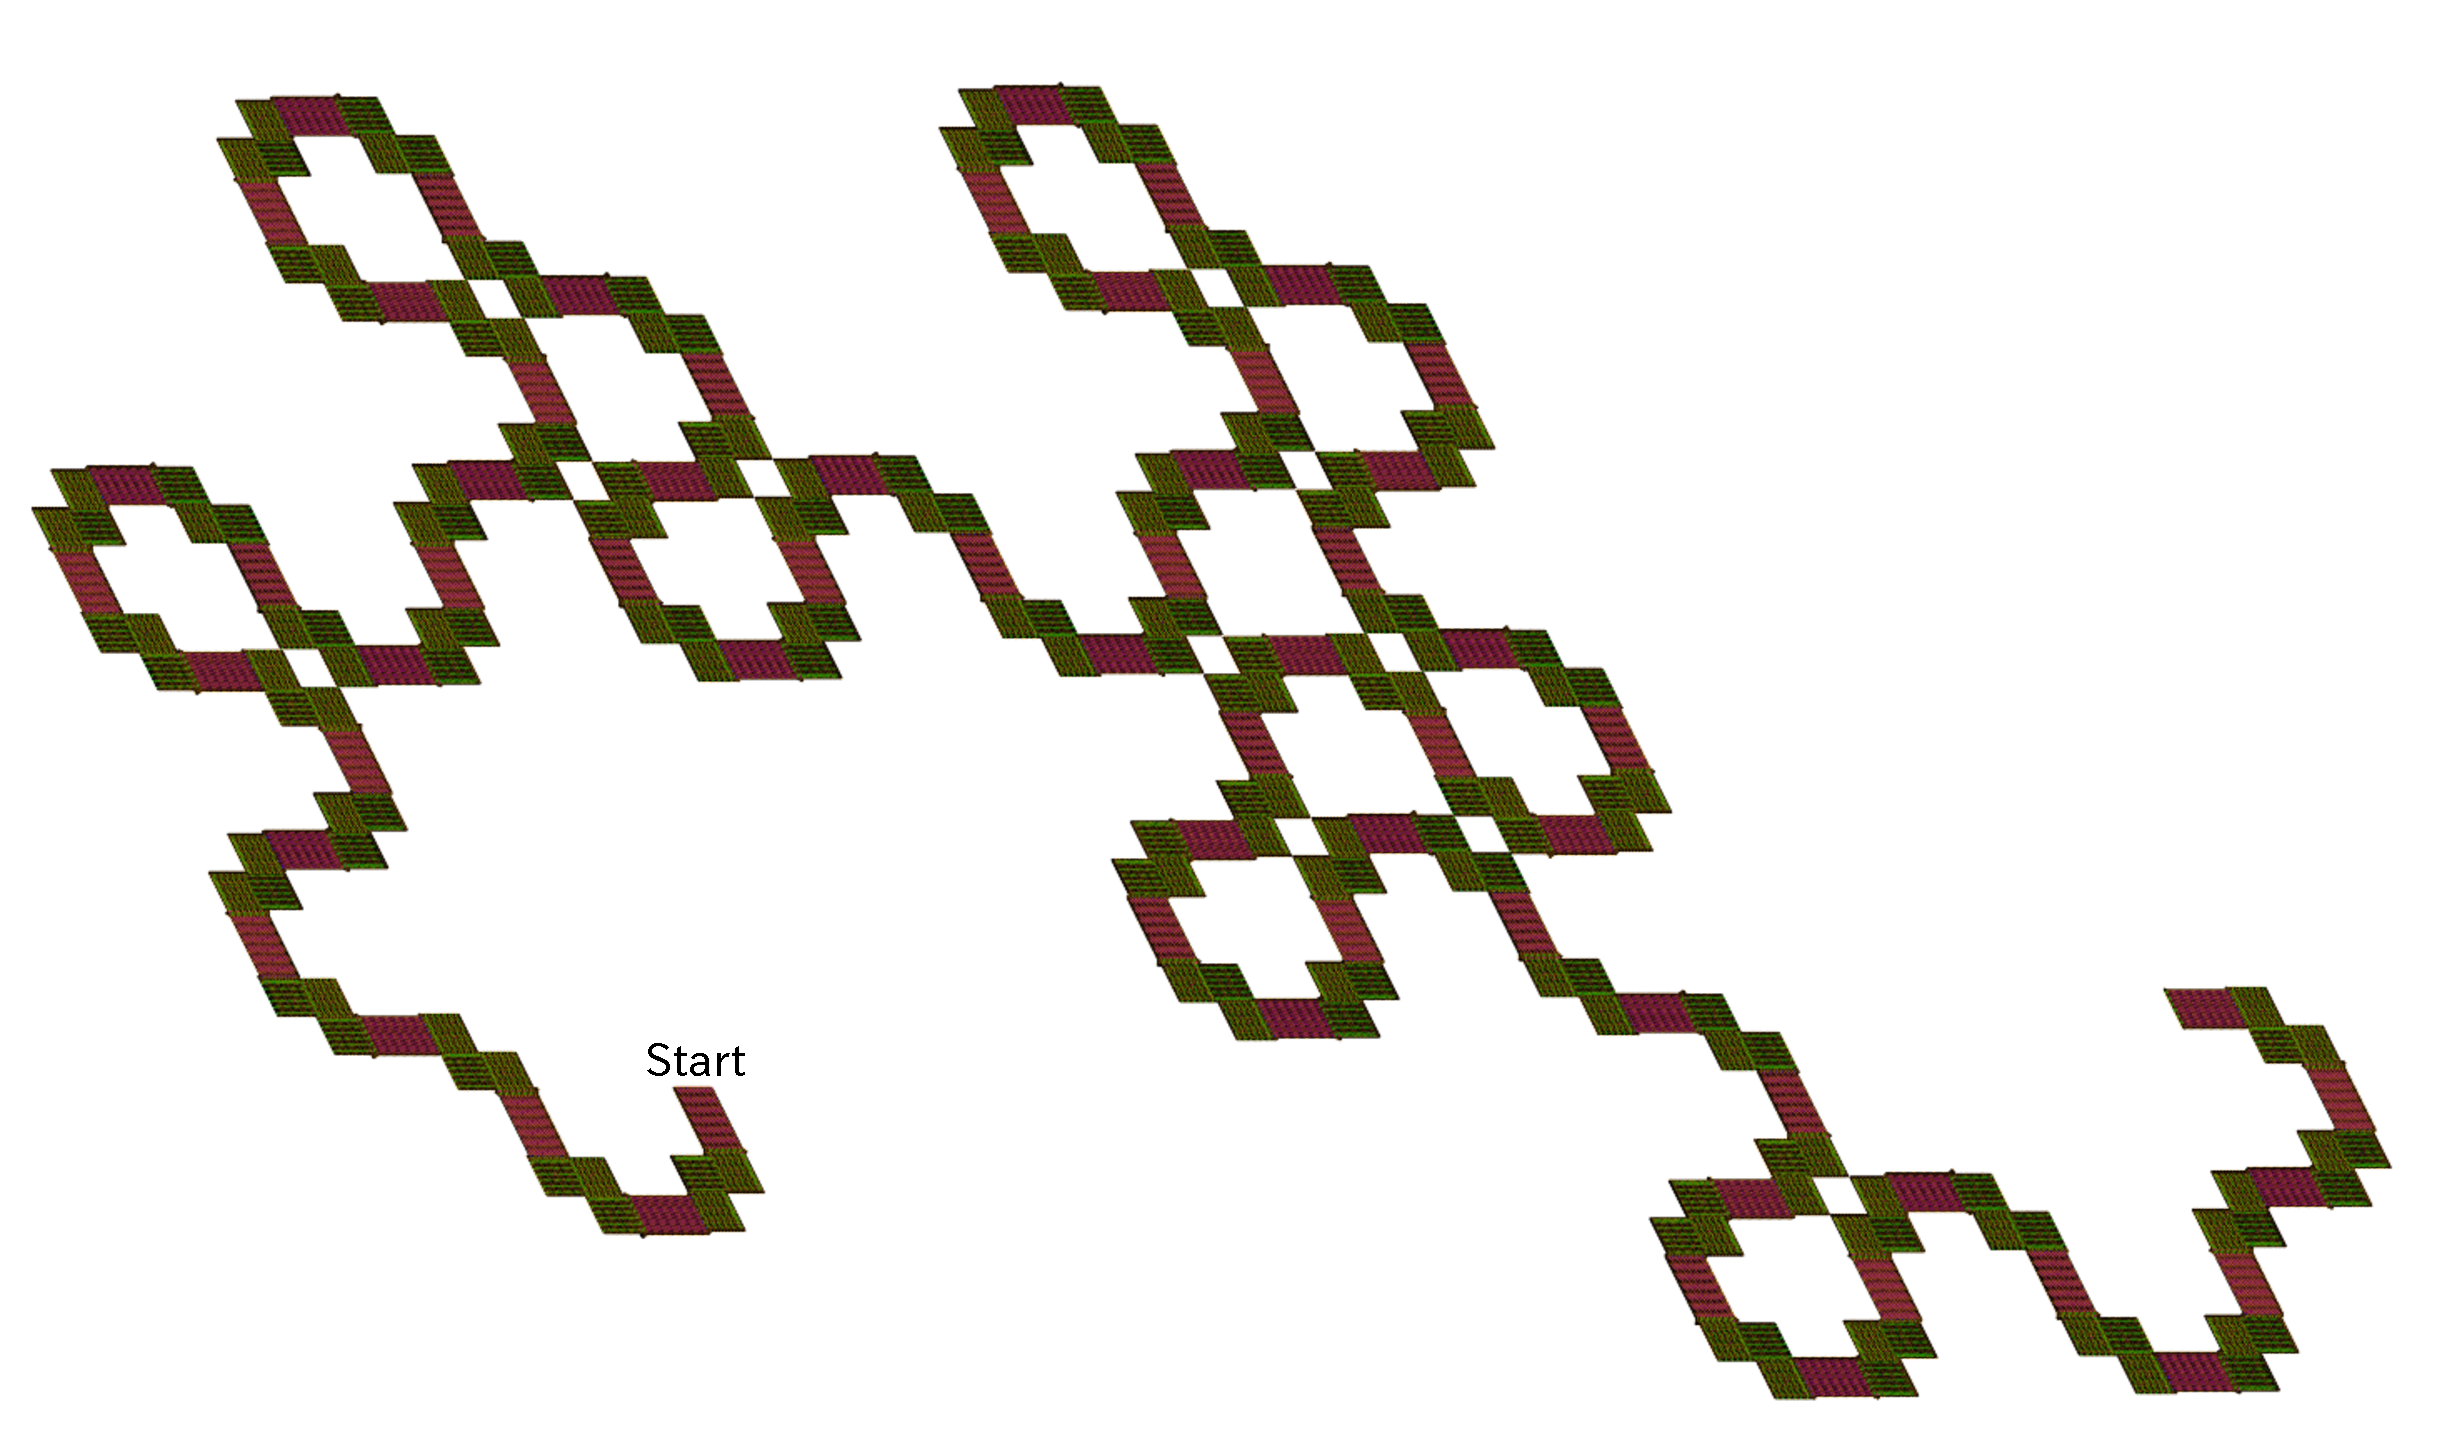
\includegraphics[width=0.7\linewidth]{6bit.pdf}
	}
	\caption{6-bit Heighway dragon by the proposed Oritatami system.}
\end{figure}

\end{frame}
%%%%%%%%%%%%%%%%%%%%%%%%%%%%%%%%%%%%%%%%%%%%%%%%%%%%%%%%%%%%%%%%%%
\begin{frame}\frametitle{Fractals and DFAO}
\begin{block}{Automatic sequences}
Heighway dragon can be represented by the Paperfolding sequence $P$, which can be output by a DFAO.
\end{block}

\begin{figure}
\begin{tabular}{c}
\begin{minipage}{0.65\hsize}
\begin{figure}
\centering
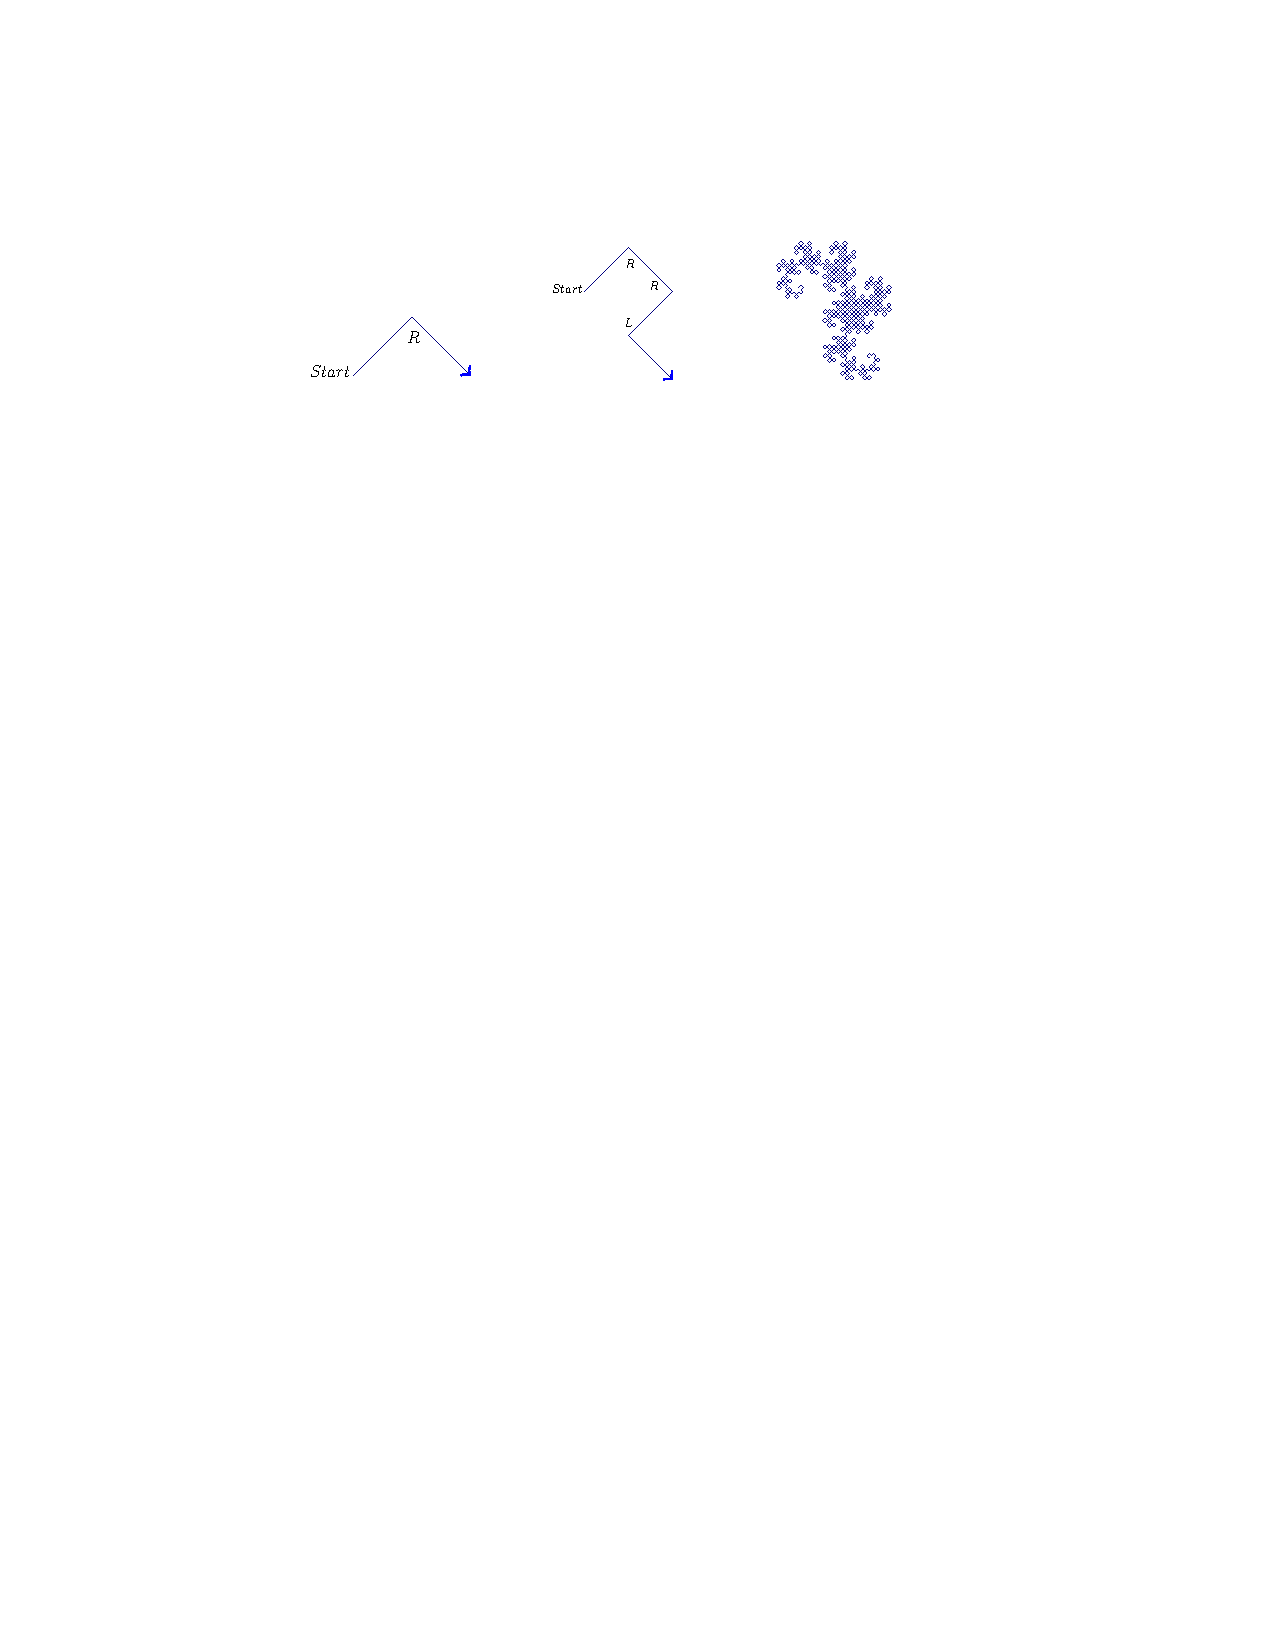
\includegraphics[width=\linewidth]{heighway_sequence.pdf} 
\end{figure}
\end{minipage}

\begin{minipage}{0.25\hsize}
\begin{figure}
  	\centering
	\scalebox{0.65}{
	\begin{tikzpicture}[>=latex, node distance=2cm,  initial text=, bend angle=15]
		 \tikzstyle{every initial by arrow} = [->, double];

		 \node [state, initial] (A)                         {$q_0/R$};
		 \node [state]                     (B) [right of = A]  {$q_1/R$};
		 \node [state]                     (C) [below right of = B] {$q_2/L$};
		 \node [state]                     (D) [above right of = B] {$q_3/R$};


 		\path [->] (A) edge [right] node [above]              {$0$}                 (B)
         		         edge [loop above] node [above]             {$1$}               ()
         			   (B) edge [bend left] node [above]             {$0$}                 (D)
         		         edge [bend right] node [below]             {$1$}              (C)
         			   (C)  edge [loop above] node [above]             {$0,1$}               ()
         			   (D)  edge [loop above] node [above]             {$0,1$}               ();
	\end{tikzpicture}
	}
\end{figure}

\end{minipage}
\end{tabular}
\caption{Paperfolding sequence $P$ = RRLRRLLR$\cdots$}
\end{figure}


\end{frame}


%%%%%%%%%%%%%%%%%%%%%%%%%%%%%%%%%%%%%%%%%%%%%%%%%%%%%%%%%%%%%%%%%%
%
%\begin{frame}\frametitle{Fractals and DFAO}
%\begin{block}{Automatic sequences}
%Heighway dragon can be represented by binary sequences (Paperfolding sequences), which can be output by DFAO.
%\end{block}
%
%\begin{figure}
%  	\centering
%	\scalebox{0.65}{
%	\begin{tikzpicture}[>=latex, node distance=2cm,  initial text=, bend angle=15]
%		 \tikzstyle{every initial by arrow} = [->, double];
%
%		 \node [state, initial] (A)                         {$A/R$};
%		 \node [state]                     (B) [right of = A]  {$B/R$};
%		 \node [state]                     (C) [below right of = B] {$C/L$};
%		 \node [state]                     (D) [above right of = B] {$D/R$};
%
%
% 		\path [->] (A) edge [right] node [above]              {$0$}                 (B)
%         		         edge [loop above] node [above]             {$1$}               ()
%         			   (B) edge [bend left] node [above]             {$0$}                 (D)
%         		         edge [bend right] node [below]             {$1$}              (C)
%         			   (C)  edge [loop above] node [above]             {$0,1$}               ()
%         			   (D)  edge [loop above] node [above]             {$0,1$}               ();
%	\end{tikzpicture}
%	}
%\caption{Paperfolding sequence $P$ = RRLRRLLR$\cdots$}
%\end{figure}
%
%\end{frame}
%%%%%%%%%%%%%%%%%%%%%%%%%%%%%%%%%%%%%%%%%%%%%%%%%%%%%%%%%%%%%%%%%%

\begin{frame}\frametitle{Fractals and DFAO}
\begin{itemize}
\only<1,2,5-6,8>{\item {\footnotesize Paperfolding sequence $P = {\rm RRLRRLLRRRLLRLLRRRLRRLLLRRLLRLL} \cdots$}}
\only<3>{\item {\footnotesize Paperfolding sequence $P = {\rm {\color{red}R}RLRRLLRRRLLRLLRRRLRRLLLRRLLRLL} \cdots$}}
\only<4>{\item {\footnotesize Paperfolding sequence $P = {\rm R{\color{red}R}LRRLLRRRLLRLLRRRLRRLLLRRLLRLL} \cdots$}}
\only<7>{\item {\footnotesize Paperfolding sequence $P = {\rm RR{\color{red}L}RRLLRRRLLRLLRRRLRRLLLRRLLRLL} \cdots$}}
\end{itemize}
\uncover<2-7>{$i=$}
\only<2,3>{$0$}
\only<4>{$1$}
\only<5,6,7>{$2 \rightarrow10$}

\vspace*{3mm}

\begin{minipage}{0.5\linewidth}{\footnotesize 
The $i$-th element of $P$ ($i \ge 0$) can be computed by 
\begin{enumerate}
\item feeding the DFA shown right with the binary representation of $i$ from its {\color{red}LSB}, and 
\item reading R/L assigned to the reached state. 
\end{enumerate}

}\end{minipage}
\begin{minipage}{0.05\linewidth}
\ \\
\end{minipage}
\begin{minipage}{0.4\linewidth}
\centering
\scalebox{0.7}{\begin{tikzpicture}[>=latex, node distance=2cm, initial text=, bend angle=15]
	\tikzstyle{every initial by arrow} = [->, double];

	\node [state, initial] (q_0)                        {$q_0/R$};
	\uncover<2,4,5>{\node [state, initial,red] (q_0)                        {$q_0/R$};}

	\node [state]                     (q_1) [right of = q_0]  {$q_1/R$};
	\uncover<3,6>{\node [state,red]                     (q_1) [right of = q_0]  {$q_1/R$};}

	\node [state]                     (q_2) [below right of = q_1] {$q_2/L$};
	\uncover<7>{\node [state,red]                     (q_2) [below right of = q_1] {$q_2/L$};}
	\node [state]                     (q_3) [above right of = q_1] {$q_3/R$};

	\path [->] (q_0) edge [right] node [above]              {$0$}                 (q_1)
         		         edge [loop above] node [above]             {$1$}               ()
         			   (q_1) edge [bend left] node [above]             {$0$}                 (q_3)
         		         edge [bend right] node [below]             {$1$}              (q_2)
         			   (q_2)  edge [loop above] node [above]             {$0,1$}               ()
         			   (q_3)  edge [loop above] node [above]             {$0,1$}               ();
\end{tikzpicture}}
\end{minipage}

\end{frame}

%%%%%%%%%%%%%%%%%%%%%%%%%%%%%%%%%%%%%%%%%%%%%%%%%%%%%%%%%%%%%%%%%%

\frame{
\frametitle{Implementation}
\framesubtitle{Problems}

Over the triangular grid, it is more natural to consider the slanted Heighway dragon. 

\vspace*{3mm}

\begin{minipage}{0.4\linewidth}
\centering
\scalebox{0.5}{\begin{tikzpicture}
\draw[-latex, rounded corners] (0, 0) 
-- ++(300:1)
-- ++(180:1)
-- ++(120:1)
-- ++(180:1)
-- ++(120:1)
-- ++(0:1)
-- ++(120:1)
-- ++(180:1)
-- ++(120:1)
-- ++(0:1)
-- ++(300:1)
-- ++(0:1)
-- ++(120:1)
-- ++(0:1)
-- ++(120:1)
-- ++(180:1)
-- ++(120:1)
-- ++(0:1)
-- ++(300:1)
-- ++(0:1)
-- ++(300:1)
-- ++(180:1)
-- ++(300:1)
-- ++(0:1)
-- ++(120:1)
-- ++(0:1)
-- ++(300:1)
-- ++(0:1)
-- ++(120:1)
-- ++(0:1)
-- ++(120:1)
-- ++(180:1)
-- ++(120:1)
-- ++(0:1)
-- ++(300:1)
-- ++(0:1)
-- ++(300:1)
-- ++(180:1)
-- ++(300:1)
-- ++(0:1)
-- ++(300:1)
-- ++(180:1)
-- ++(120:1)
-- ++(180:1)
-- ++(300:1)
-- ++(180:1)
-- ++(300:1)
-- ++(0:1)
-- ++(120:1)
-- ++(0:1)
-- ++(300:1)
-- ++(0:1)
-- ++(300:1)
-- ++(180:1)
-- ++(300:1)
-- ++(0:1)
-- ++(120:1)
-- ++(0:1)
-- ++(300:1)
-- ++(0:1)
-- ++(120:1)
-- ++(0:1)
-- ++(120:1)
-- ++(180:1)
;

\uncover<2->{\draw[orange, thick] (0.125,0) -- ++(120:0.125) -- ++(180:0.25) -- ++(300:0.25) -- ++(0:0.25) -- ++(120:0.125) 
++(300:0.25) -- ++(120:0.125) -- ++(180:0.25) -- ++(300:0.25) -- ++(0:0.25) -- ++(120:0.125)
++(300:0.25) -- ++(120:0.125) -- ++(180:0.25) -- ++(300:0.25) -- ++(0:0.25) -- ++(120:0.125)
++(300:0.25) -- ++(120:0.125) -- ++(180:0.25) -- ++(300:0.25) -- ++(0:0.25) -- ++(120:0.125)
++(300:0.25) -- ++(120:0.125) -- ++(180:0.25) -- ++(300:0.25) -- ++(0:0.25) -- ++(120:0.125)
++(180:0.25) -- ++(120:0.125) -- ++(180:0.25) -- ++(300:0.25) -- ++(0:0.25) -- ++(120:0.125)
++(180:0.25) -- ++(120:0.125) -- ++(180:0.25) -- ++(300:0.25) -- ++(0:0.25) -- ++(120:0.125)
++(180:0.25) -- ++(120:0.125) -- ++(180:0.25) -- ++(300:0.25) -- ++(0:0.25) -- ++(120:0.125)
++(180:0.25) -- ++(120:0.125) -- ++(180:0.25) -- ++(300:0.25) -- ++(0:0.25) -- ++(120:0.125)
++(120:0.25) -- ++(120:0.125) -- ++(180:0.25) -- ++(300:0.25) -- ++(0:0.25) -- ++(120:0.125)
++(120:0.25) -- ++(120:0.125) -- ++(180:0.25) -- ++(300:0.25) -- ++(0:0.25) -- ++(120:0.125)
++(120:0.25) -- ++(120:0.125) -- ++(180:0.25) -- ++(300:0.25) -- ++(0:0.25) -- ++(120:0.125)
++(120:0.25) -- ++(120:0.125) -- ++(180:0.25) -- ++(300:0.25) -- ++(0:0.25) -- ++(120:0.125)
++(180:0.25) -- ++(120:0.125) -- ++(180:0.25) -- ++(300:0.25) -- ++(0:0.25) -- ++(120:0.125)
++(180:0.25) -- ++(120:0.125) -- ++(180:0.25) -- ++(300:0.25) -- ++(0:0.25) -- ++(120:0.125)
++(180:0.25) -- ++(120:0.125) -- ++(180:0.25) -- ++(300:0.25) -- ++(0:0.25) -- ++(120:0.125)
++(180:0.25) -- ++(120:0.125) -- ++(180:0.25) -- ++(300:0.25) -- ++(0:0.25) -- ++(120:0.125)
++(120:0.25) -- ++(120:0.125) -- ++(180:0.25) -- ++(300:0.25) -- ++(0:0.25) -- ++(120:0.125)
++(120:0.25) -- ++(120:0.125) -- ++(180:0.25) -- ++(300:0.25) -- ++(0:0.25) -- ++(120:0.125)
++(120:0.25) -- ++(120:0.125) -- ++(180:0.25) -- ++(300:0.25) -- ++(0:0.25) -- ++(120:0.125)
++(120:0.25) -- ++(120:0.125) -- ++(180:0.25) -- ++(300:0.25) -- ++(0:0.25) -- ++(120:0.125)
++(0:0.25) -- ++(120:0.125) -- ++(180:0.25) -- ++(300:0.25) -- ++(0:0.25) -- ++(120:0.125)
++(0:0.25) -- ++(120:0.125) -- ++(180:0.25) -- ++(300:0.25) -- ++(0:0.25) -- ++(120:0.125)
++(0:0.25) -- ++(120:0.125) -- ++(180:0.25) -- ++(300:0.25) -- ++(0:0.25) -- ++(120:0.125)
++(0:0.25) -- ++(120:0.125) -- ++(180:0.25) -- ++(300:0.25) -- ++(0:0.25) -- ++(120:0.125)
++(120:0.25) -- ++(120:0.125) -- ++(180:0.25) -- ++(300:0.25) -- ++(0:0.25) -- ++(120:0.125)
++(120:0.25) -- ++(120:0.125) -- ++(180:0.25) -- ++(300:0.25) -- ++(0:0.25) -- ++(120:0.125)
++(120:0.25) -- ++(120:0.125) -- ++(180:0.25) -- ++(300:0.25) -- ++(0:0.25) -- ++(120:0.125)
++(120:0.25) -- ++(120:0.125) -- ++(180:0.25) -- ++(300:0.25) -- ++(0:0.25) -- ++(120:0.125)
++(180:0.25) -- ++(120:0.125) -- ++(180:0.25) -- ++(300:0.25) -- ++(0:0.25) -- ++(120:0.125)
++(180:0.25) -- ++(120:0.125) -- ++(180:0.25) -- ++(300:0.25) -- ++(0:0.25) -- ++(120:0.125)
++(180:0.25) -- ++(120:0.125) -- ++(180:0.25) -- ++(300:0.25) -- ++(0:0.25) -- ++(120:0.125)
++(180:0.25) -- ++(120:0.125) -- ++(180:0.25) -- ++(300:0.25) -- ++(0:0.25) -- ++(120:0.125)
++(120:0.25) -- ++(120:0.125) -- ++(180:0.25) -- ++(300:0.25) -- ++(0:0.25) -- ++(120:0.125)
++(120:0.25) -- ++(120:0.125) -- ++(180:0.25) -- ++(300:0.25) -- ++(0:0.25) -- ++(120:0.125)
++(120:0.25) -- ++(120:0.125) -- ++(180:0.25) -- ++(300:0.25) -- ++(0:0.25) -- ++(120:0.125)
++(120:0.25) -- ++(120:0.125) -- ++(180:0.25) -- ++(300:0.25) -- ++(0:0.25) -- ++(120:0.125)
++(0:0.25) -- ++(120:0.125) -- ++(180:0.25) -- ++(300:0.25) -- ++(0:0.25) -- ++(120:0.125)
++(0:0.25) -- ++(120:0.125) -- ++(180:0.25) -- ++(300:0.25) -- ++(0:0.25) -- ++(120:0.125)
++(0:0.25) -- ++(120:0.125) -- ++(180:0.25) -- ++(300:0.25) -- ++(0:0.25) -- ++(120:0.125)
++(0:0.25) -- ++(120:0.125) -- ++(180:0.25) -- ++(300:0.25) -- ++(0:0.25) -- ++(120:0.125)
++(300:0.25) -- ++(120:0.125) -- ++(180:0.25) -- ++(300:0.25) -- ++(0:0.25) -- ++(120:0.125)
++(300:0.25) -- ++(120:0.125) -- ++(180:0.25) -- ++(300:0.25) -- ++(0:0.25) -- ++(120:0.125)
++(300:0.25) -- ++(120:0.125) -- ++(180:0.25) -- ++(300:0.25) -- ++(0:0.25) -- ++(120:0.125)
++(300:0.25) -- ++(120:0.125) -- ++(180:0.25) -- ++(300:0.25) -- ++(0:0.25) -- ++(120:0.125)
++(0:0.25) -- ++(120:0.125) -- ++(180:0.25) -- ++(300:0.25) -- ++(0:0.25) -- ++(120:0.125)
++(0:0.25) -- ++(120:0.125) -- ++(180:0.25) -- ++(300:0.25) -- ++(0:0.25) -- ++(120:0.125)
++(0:0.25) -- ++(120:0.125) -- ++(180:0.25) -- ++(300:0.25) -- ++(0:0.25) -- ++(120:0.125)
++(0:0.25) -- ++(120:0.125) -- ++(180:0.25) -- ++(300:0.25) -- ++(0:0.25) -- ++(120:0.125)
++(120:0.25) -- ++(120:0.125) -- ++(180:0.25) -- ++(300:0.25) -- ++(0:0.25) -- ++(120:0.125)
++(120:0.25) -- ++(120:0.125) -- ++(180:0.25) -- ++(300:0.25) -- ++(0:0.25) -- ++(120:0.125)
++(120:0.25) -- ++(120:0.125) -- ++(180:0.25) -- ++(300:0.25) -- ++(0:0.25) -- ++(120:0.125)
++(120:0.25) -- ++(120:0.125) -- ++(180:0.25) -- ++(300:0.25) -- ++(0:0.25) -- ++(120:0.125)
++(0:0.25) -- ++(120:0.125) -- ++(180:0.25) -- ++(300:0.25) -- ++(0:0.25) -- ++(120:0.125)
++(0:0.25) -- ++(120:0.125) -- ++(180:0.25) -- ++(300:0.25) -- ++(0:0.25) -- ++(120:0.125)
++(0:0.25) -- ++(120:0.125) -- ++(180:0.25) -- ++(300:0.25) -- ++(0:0.25) -- ++(120:0.125)
++(0:0.25) -- ++(120:0.125) -- ++(180:0.25) -- ++(300:0.25) -- ++(0:0.25) -- ++(120:0.125)
++(120:0.25) -- ++(120:0.125) -- ++(180:0.25) -- ++(300:0.25) -- ++(0:0.25) -- ++(120:0.125)
++(120:0.25) -- ++(120:0.125) -- ++(180:0.25) -- ++(300:0.25) -- ++(0:0.25) -- ++(120:0.125)
++(120:0.25) -- ++(120:0.125) -- ++(180:0.25) -- ++(300:0.25) -- ++(0:0.25) -- ++(120:0.125)
++(120:0.25) -- ++(120:0.125) -- ++(180:0.25) -- ++(300:0.25) -- ++(0:0.25) -- ++(120:0.125)
++(180:0.25) -- ++(120:0.125) -- ++(180:0.25) -- ++(300:0.25) -- ++(0:0.25) -- ++(120:0.125)
++(180:0.25) -- ++(120:0.125) -- ++(180:0.25) -- ++(300:0.25) -- ++(0:0.25) -- ++(120:0.125)
++(180:0.25) -- ++(120:0.125) -- ++(180:0.25) -- ++(300:0.25) -- ++(0:0.25) -- ++(120:0.125)
++(180:0.25) -- ++(120:0.125) -- ++(180:0.25) -- ++(300:0.25) -- ++(0:0.25) -- ++(120:0.125)
++(120:0.25) -- ++(120:0.125) -- ++(180:0.25) -- ++(300:0.25) -- ++(0:0.25) -- ++(120:0.125)
++(120:0.25) -- ++(120:0.125) -- ++(180:0.25) -- ++(300:0.25) -- ++(0:0.25) -- ++(120:0.125)
++(120:0.25) -- ++(120:0.125) -- ++(180:0.25) -- ++(300:0.25) -- ++(0:0.25) -- ++(120:0.125)
++(120:0.25) -- ++(120:0.125) -- ++(180:0.25) -- ++(300:0.25) -- ++(0:0.25) -- ++(120:0.125)
++(0:0.25) -- ++(120:0.125) -- ++(180:0.25) -- ++(300:0.25) -- ++(0:0.25) -- ++(120:0.125)
++(0:0.25) -- ++(120:0.125) -- ++(180:0.25) -- ++(300:0.25) -- ++(0:0.25) -- ++(120:0.125)
++(0:0.25) -- ++(120:0.125) -- ++(180:0.25) -- ++(300:0.25) -- ++(0:0.25) -- ++(120:0.125)
++(0:0.25) -- ++(120:0.125) -- ++(180:0.25) -- ++(300:0.25) -- ++(0:0.25) -- ++(120:0.125)
++(300:0.25) -- ++(120:0.125) -- ++(180:0.25) -- ++(300:0.25) -- ++(0:0.25) -- ++(120:0.125)
++(300:0.25) -- ++(120:0.125) -- ++(180:0.25) -- ++(300:0.25) -- ++(0:0.25) -- ++(120:0.125)
++(300:0.25) -- ++(120:0.125) -- ++(180:0.25) -- ++(300:0.25) -- ++(0:0.25) -- ++(120:0.125)
++(300:0.25) -- ++(120:0.125) -- ++(180:0.25) -- ++(300:0.25) -- ++(0:0.25) -- ++(120:0.125)
++(0:0.25) -- ++(120:0.125) -- ++(180:0.25) -- ++(300:0.25) -- ++(0:0.25) -- ++(120:0.125)
++(0:0.25) -- ++(120:0.125) -- ++(180:0.25) -- ++(300:0.25) -- ++(0:0.25) -- ++(120:0.125)
++(0:0.25) -- ++(120:0.125) -- ++(180:0.25) -- ++(300:0.25) -- ++(0:0.25) -- ++(120:0.125)
++(0:0.25) -- ++(120:0.125) -- ++(180:0.25) -- ++(300:0.25) -- ++(0:0.25) -- ++(120:0.125)
++(300:0.25) -- ++(120:0.125) -- ++(180:0.25) -- ++(300:0.25) -- ++(0:0.25) -- ++(120:0.125)
++(300:0.25) -- ++(120:0.125) -- ++(180:0.25) -- ++(300:0.25) -- ++(0:0.25) -- ++(120:0.125)
++(300:0.25) -- ++(120:0.125) -- ++(180:0.25) -- ++(300:0.25) -- ++(0:0.25) -- ++(120:0.125)
++(300:0.25) -- ++(120:0.125) -- ++(180:0.25) -- ++(300:0.25) -- ++(0:0.25) -- ++(120:0.125)
++(180:0.25) -- ++(120:0.125) -- ++(180:0.25) -- ++(300:0.25) -- ++(0:0.25) -- ++(120:0.125)
++(180:0.25) -- ++(120:0.125) -- ++(180:0.25) -- ++(300:0.25) -- ++(0:0.25) -- ++(120:0.125)
++(180:0.25) -- ++(120:0.125) -- ++(180:0.25) -- ++(300:0.25) -- ++(0:0.25) -- ++(120:0.125)
++(180:0.25) -- ++(120:0.125) -- ++(180:0.25) -- ++(300:0.25) -- ++(0:0.25) -- ++(120:0.125)
++(300:0.25) -- ++(120:0.125) -- ++(180:0.25) -- ++(300:0.25) -- ++(0:0.25) -- ++(120:0.125)
++(300:0.25) -- ++(120:0.125) -- ++(180:0.25) -- ++(300:0.25) -- ++(0:0.25) -- ++(120:0.125)
++(300:0.25) -- ++(120:0.125) -- ++(180:0.25) -- ++(300:0.25) -- ++(0:0.25) -- ++(120:0.125)
++(300:0.25) -- ++(120:0.125) -- ++(180:0.25) -- ++(300:0.25) -- ++(0:0.25) -- ++(120:0.125)
++(0:0.25) -- ++(120:0.125) -- ++(180:0.25) -- ++(300:0.25) -- ++(0:0.25) -- ++(120:0.125)
++(0:0.25) -- ++(120:0.125) -- ++(180:0.25) -- ++(300:0.25) -- ++(0:0.25) -- ++(120:0.125)
++(0:0.25) -- ++(120:0.125) -- ++(180:0.25) -- ++(300:0.25) -- ++(0:0.25) -- ++(120:0.125)
++(0:0.25) -- ++(120:0.125) -- ++(180:0.25) -- ++(300:0.25) -- ++(0:0.25) -- ++(120:0.125)
++(120:0.25) -- ++(120:0.125) -- ++(180:0.25) -- ++(300:0.25) -- ++(0:0.25) -- ++(120:0.125)
++(120:0.25) -- ++(120:0.125) -- ++(180:0.25) -- ++(300:0.25) -- ++(0:0.25) -- ++(120:0.125)
++(120:0.25) -- ++(120:0.125) -- ++(180:0.25) -- ++(300:0.25) -- ++(0:0.25) -- ++(120:0.125)
++(120:0.25) -- ++(120:0.125) -- ++(180:0.25) -- ++(300:0.25) -- ++(0:0.25) -- ++(120:0.125)
++(0:0.25) -- ++(120:0.125) -- ++(180:0.25) -- ++(300:0.25) -- ++(0:0.25) -- ++(120:0.125)
++(0:0.25) -- ++(120:0.125) -- ++(180:0.25) -- ++(300:0.25) -- ++(0:0.25) -- ++(120:0.125)
++(0:0.25) -- ++(120:0.125) -- ++(180:0.25) -- ++(300:0.25) -- ++(0:0.25) -- ++(120:0.125)
++(0:0.25) -- ++(120:0.125) -- ++(180:0.25) -- ++(300:0.25) -- ++(0:0.25) -- ++(120:0.125)
++(300:0.25) -- ++(120:0.125) -- ++(180:0.25) -- ++(300:0.25) -- ++(0:0.25) -- ++(120:0.125)
++(300:0.25) -- ++(120:0.125) -- ++(180:0.25) -- ++(300:0.25) -- ++(0:0.25) -- ++(120:0.125)
++(300:0.25) -- ++(120:0.125) -- ++(180:0.25) -- ++(300:0.25) -- ++(0:0.25) -- ++(120:0.125)
++(300:0.25) -- ++(120:0.125) -- ++(180:0.25) -- ++(300:0.25) -- ++(0:0.25) -- ++(120:0.125)
++(0:0.25) -- ++(120:0.125) -- ++(180:0.25) -- ++(300:0.25) -- ++(0:0.25) -- ++(120:0.125)
++(0:0.25) -- ++(120:0.125) -- ++(180:0.25) -- ++(300:0.25) -- ++(0:0.25) -- ++(120:0.125)
++(0:0.25) -- ++(120:0.125) -- ++(180:0.25) -- ++(300:0.25) -- ++(0:0.25) -- ++(120:0.125)
++(0:0.25) -- ++(120:0.125) -- ++(180:0.25) -- ++(300:0.25) -- ++(0:0.25) -- ++(120:0.125)
++(120:0.25) -- ++(120:0.125) -- ++(180:0.25) -- ++(300:0.25) -- ++(0:0.25) -- ++(120:0.125)
++(120:0.25) -- ++(120:0.125) -- ++(180:0.25) -- ++(300:0.25) -- ++(0:0.25) -- ++(120:0.125)
++(120:0.25) -- ++(120:0.125) -- ++(180:0.25) -- ++(300:0.25) -- ++(0:0.25) -- ++(120:0.125)
++(120:0.25) -- ++(120:0.125) -- ++(180:0.25) -- ++(300:0.25) -- ++(0:0.25) -- ++(120:0.125)
++(0:0.25) -- ++(120:0.125) -- ++(180:0.25) -- ++(300:0.25) -- ++(0:0.25) -- ++(120:0.125)
++(0:0.25) -- ++(120:0.125) -- ++(180:0.25) -- ++(300:0.25) -- ++(0:0.25) -- ++(120:0.125)
++(0:0.25) -- ++(120:0.125) -- ++(180:0.25) -- ++(300:0.25) -- ++(0:0.25) -- ++(120:0.125)
++(0:0.25) -- ++(120:0.125) -- ++(180:0.25) -- ++(300:0.25) -- ++(0:0.25) -- ++(120:0.125)
++(120:0.25) -- ++(120:0.125) -- ++(180:0.25) -- ++(300:0.25) -- ++(0:0.25) -- ++(120:0.125)
++(120:0.25) -- ++(120:0.125) -- ++(180:0.25) -- ++(300:0.25) -- ++(0:0.25) -- ++(120:0.125)
++(120:0.25) -- ++(120:0.125) -- ++(180:0.25) -- ++(300:0.25) -- ++(0:0.25) -- ++(120:0.125)
++(120:0.25) -- ++(120:0.125) -- ++(180:0.25) -- ++(300:0.25) -- ++(0:0.25) -- ++(120:0.125)
++(180:0.25) -- ++(120:0.125) -- ++(180:0.25) -- ++(300:0.25) -- ++(0:0.25) -- ++(120:0.125)
++(180:0.25) -- ++(120:0.125) -- ++(180:0.25) -- ++(300:0.25) -- ++(0:0.25) -- ++(120:0.125)
++(180:0.25) -- ++(120:0.125) -- ++(180:0.25) -- ++(300:0.25) -- ++(0:0.25) -- ++(120:0.125)
++(180:0.25) -- ++(120:0.125) -- ++(180:0.25) -- ++(300:0.25) -- ++(0:0.25) -- ++(120:0.125)
++(120:0.25) -- ++(120:0.125) -- ++(180:0.25) -- ++(300:0.25) -- ++(0:0.25) -- ++(120:0.125)
++(120:0.25) -- ++(120:0.125) -- ++(180:0.25) -- ++(300:0.25) -- ++(0:0.25) -- ++(120:0.125)
++(120:0.25) -- ++(120:0.125) -- ++(180:0.25) -- ++(300:0.25) -- ++(0:0.25) -- ++(120:0.125)
++(120:0.25) -- ++(120:0.125) -- ++(180:0.25) -- ++(300:0.25) -- ++(0:0.25) -- ++(120:0.125)
++(0:0.25) -- ++(120:0.125) -- ++(180:0.25) -- ++(300:0.25) -- ++(0:0.25) -- ++(120:0.125)
++(0:0.25) -- ++(120:0.125) -- ++(180:0.25) -- ++(300:0.25) -- ++(0:0.25) -- ++(120:0.125)
++(0:0.25) -- ++(120:0.125) -- ++(180:0.25) -- ++(300:0.25) -- ++(0:0.25) -- ++(120:0.125)
++(0:0.25) -- ++(120:0.125) -- ++(180:0.25) -- ++(300:0.25) -- ++(0:0.25) -- ++(120:0.125)
++(300:0.25) -- ++(120:0.125) -- ++(180:0.25) -- ++(300:0.25) -- ++(0:0.25) -- ++(120:0.125)
++(300:0.25) -- ++(120:0.125) -- ++(180:0.25) -- ++(300:0.25) -- ++(0:0.25) -- ++(120:0.125)
++(300:0.25) -- ++(120:0.125) -- ++(180:0.25) -- ++(300:0.25) -- ++(0:0.25) -- ++(120:0.125)
++(300:0.25) -- ++(120:0.125) -- ++(180:0.25) -- ++(300:0.25) -- ++(0:0.25) -- ++(120:0.125)
++(0:0.25) -- ++(120:0.125) -- ++(180:0.25) -- ++(300:0.25) -- ++(0:0.25) -- ++(120:0.125)
++(0:0.25) -- ++(120:0.125) -- ++(180:0.25) -- ++(300:0.25) -- ++(0:0.25) -- ++(120:0.125)
++(0:0.25) -- ++(120:0.125) -- ++(180:0.25) -- ++(300:0.25) -- ++(0:0.25) -- ++(120:0.125)
++(0:0.25) -- ++(120:0.125) -- ++(180:0.25) -- ++(300:0.25) -- ++(0:0.25) -- ++(120:0.125)
++(300:0.25) -- ++(120:0.125) -- ++(180:0.25) -- ++(300:0.25) -- ++(0:0.25) -- ++(120:0.125)
++(300:0.25) -- ++(120:0.125) -- ++(180:0.25) -- ++(300:0.25) -- ++(0:0.25) -- ++(120:0.125)
++(300:0.25) -- ++(120:0.125) -- ++(180:0.25) -- ++(300:0.25) -- ++(0:0.25) -- ++(120:0.125)
++(300:0.25) -- ++(120:0.125) -- ++(180:0.25) -- ++(300:0.25) -- ++(0:0.25) -- ++(120:0.125)
++(180:0.25) -- ++(120:0.125) -- ++(180:0.25) -- ++(300:0.25) -- ++(0:0.25) -- ++(120:0.125)
++(180:0.25) -- ++(120:0.125) -- ++(180:0.25) -- ++(300:0.25) -- ++(0:0.25) -- ++(120:0.125)
++(180:0.25) -- ++(120:0.125) -- ++(180:0.25) -- ++(300:0.25) -- ++(0:0.25) -- ++(120:0.125)
++(180:0.25) -- ++(120:0.125) -- ++(180:0.25) -- ++(300:0.25) -- ++(0:0.25) -- ++(120:0.125)
++(300:0.25) -- ++(120:0.125) -- ++(180:0.25) -- ++(300:0.25) -- ++(0:0.25) -- ++(120:0.125)
++(300:0.25) -- ++(120:0.125) -- ++(180:0.25) -- ++(300:0.25) -- ++(0:0.25) -- ++(120:0.125)
++(300:0.25) -- ++(120:0.125) -- ++(180:0.25) -- ++(300:0.25) -- ++(0:0.25) -- ++(120:0.125)
++(300:0.25) -- ++(120:0.125) -- ++(180:0.25) -- ++(300:0.25) -- ++(0:0.25) -- ++(120:0.125)
++(0:0.25) -- ++(120:0.125) -- ++(180:0.25) -- ++(300:0.25) -- ++(0:0.25) -- ++(120:0.125)
++(0:0.25) -- ++(120:0.125) -- ++(180:0.25) -- ++(300:0.25) -- ++(0:0.25) -- ++(120:0.125)
++(0:0.25) -- ++(120:0.125) -- ++(180:0.25) -- ++(300:0.25) -- ++(0:0.25) -- ++(120:0.125)
++(0:0.25) -- ++(120:0.125) -- ++(180:0.25) -- ++(300:0.25) -- ++(0:0.25) -- ++(120:0.125)
++(300:0.25) -- ++(120:0.125) -- ++(180:0.25) -- ++(300:0.25) -- ++(0:0.25) -- ++(120:0.125)
++(300:0.25) -- ++(120:0.125) -- ++(180:0.25) -- ++(300:0.25) -- ++(0:0.25) -- ++(120:0.125)
++(300:0.25) -- ++(120:0.125) -- ++(180:0.25) -- ++(300:0.25) -- ++(0:0.25) -- ++(120:0.125)
++(300:0.25) -- ++(120:0.125) -- ++(180:0.25) -- ++(300:0.25) -- ++(0:0.25) -- ++(120:0.125)
++(180:0.25) -- ++(120:0.125) -- ++(180:0.25) -- ++(300:0.25) -- ++(0:0.25) -- ++(120:0.125)
++(180:0.25) -- ++(120:0.125) -- ++(180:0.25) -- ++(300:0.25) -- ++(0:0.25) -- ++(120:0.125)
++(180:0.25) -- ++(120:0.125) -- ++(180:0.25) -- ++(300:0.25) -- ++(0:0.25) -- ++(120:0.125)
++(180:0.25) -- ++(120:0.125) -- ++(180:0.25) -- ++(300:0.25) -- ++(0:0.25) -- ++(120:0.125)
++(120:0.25) -- ++(120:0.125) -- ++(180:0.25) -- ++(300:0.25) -- ++(0:0.25) -- ++(120:0.125)
++(120:0.25) -- ++(120:0.125) -- ++(180:0.25) -- ++(300:0.25) -- ++(0:0.25) -- ++(120:0.125)
++(120:0.25) -- ++(120:0.125) -- ++(180:0.25) -- ++(300:0.25) -- ++(0:0.25) -- ++(120:0.125)
++(120:0.25) -- ++(120:0.125) -- ++(180:0.25) -- ++(300:0.25) -- ++(0:0.25) -- ++(120:0.125)
++(180:0.25) -- ++(120:0.125) -- ++(180:0.25) -- ++(300:0.25) -- ++(0:0.25) -- ++(120:0.125)
++(180:0.25) -- ++(120:0.125) -- ++(180:0.25) -- ++(300:0.25) -- ++(0:0.25) -- ++(120:0.125)
++(180:0.25) -- ++(120:0.125) -- ++(180:0.25) -- ++(300:0.25) -- ++(0:0.25) -- ++(120:0.125)
++(180:0.25) -- ++(120:0.125) -- ++(180:0.25) -- ++(300:0.25) -- ++(0:0.25) -- ++(120:0.125)
++(300:0.25) -- ++(120:0.125) -- ++(180:0.25) -- ++(300:0.25) -- ++(0:0.25) -- ++(120:0.125)
++(300:0.25) -- ++(120:0.125) -- ++(180:0.25) -- ++(300:0.25) -- ++(0:0.25) -- ++(120:0.125)
++(300:0.25) -- ++(120:0.125) -- ++(180:0.25) -- ++(300:0.25) -- ++(0:0.25) -- ++(120:0.125)
++(300:0.25) -- ++(120:0.125) -- ++(180:0.25) -- ++(300:0.25) -- ++(0:0.25) -- ++(120:0.125)
++(180:0.25) -- ++(120:0.125) -- ++(180:0.25) -- ++(300:0.25) -- ++(0:0.25) -- ++(120:0.125)
++(180:0.25) -- ++(120:0.125) -- ++(180:0.25) -- ++(300:0.25) -- ++(0:0.25) -- ++(120:0.125)
++(180:0.25) -- ++(120:0.125) -- ++(180:0.25) -- ++(300:0.25) -- ++(0:0.25) -- ++(120:0.125)
++(180:0.25) -- ++(120:0.125) -- ++(180:0.25) -- ++(300:0.25) -- ++(0:0.25) -- ++(120:0.125)
++(300:0.25) -- ++(120:0.125) -- ++(180:0.25) -- ++(300:0.25) -- ++(0:0.25) -- ++(120:0.125)
++(300:0.25) -- ++(120:0.125) -- ++(180:0.25) -- ++(300:0.25) -- ++(0:0.25) -- ++(120:0.125)
++(300:0.25) -- ++(120:0.125) -- ++(180:0.25) -- ++(300:0.25) -- ++(0:0.25) -- ++(120:0.125)
++(300:0.25) -- ++(120:0.125) -- ++(180:0.25) -- ++(300:0.25) -- ++(0:0.25) -- ++(120:0.125)
++(0:0.25) -- ++(120:0.125) -- ++(180:0.25) -- ++(300:0.25) -- ++(0:0.25) -- ++(120:0.125)
++(0:0.25) -- ++(120:0.125) -- ++(180:0.25) -- ++(300:0.25) -- ++(0:0.25) -- ++(120:0.125)
++(0:0.25) -- ++(120:0.125) -- ++(180:0.25) -- ++(300:0.25) -- ++(0:0.25) -- ++(120:0.125)
++(0:0.25) -- ++(120:0.125) -- ++(180:0.25) -- ++(300:0.25) -- ++(0:0.25) -- ++(120:0.125)
++(120:0.25) -- ++(120:0.125) -- ++(180:0.25) -- ++(300:0.25) -- ++(0:0.25) -- ++(120:0.125)
++(120:0.25) -- ++(120:0.125) -- ++(180:0.25) -- ++(300:0.25) -- ++(0:0.25) -- ++(120:0.125)
++(120:0.25) -- ++(120:0.125) -- ++(180:0.25) -- ++(300:0.25) -- ++(0:0.25) -- ++(120:0.125)
++(120:0.25) -- ++(120:0.125) -- ++(180:0.25) -- ++(300:0.25) -- ++(0:0.25) -- ++(120:0.125)
++(0:0.25) -- ++(120:0.125) -- ++(180:0.25) -- ++(300:0.25) -- ++(0:0.25) -- ++(120:0.125)
++(0:0.25) -- ++(120:0.125) -- ++(180:0.25) -- ++(300:0.25) -- ++(0:0.25) -- ++(120:0.125)
++(0:0.25) -- ++(120:0.125) -- ++(180:0.25) -- ++(300:0.25) -- ++(0:0.25) -- ++(120:0.125)
++(0:0.25) -- ++(120:0.125) -- ++(180:0.25) -- ++(300:0.25) -- ++(0:0.25) -- ++(120:0.125)
++(300:0.25) -- ++(120:0.125) -- ++(180:0.25) -- ++(300:0.25) -- ++(0:0.25) -- ++(120:0.125)
++(300:0.25) -- ++(120:0.125) -- ++(180:0.25) -- ++(300:0.25) -- ++(0:0.25) -- ++(120:0.125)
++(300:0.25) -- ++(120:0.125) -- ++(180:0.25) -- ++(300:0.25) -- ++(0:0.25) -- ++(120:0.125)
++(300:0.25) -- ++(120:0.125) -- ++(180:0.25) -- ++(300:0.25) -- ++(0:0.25) -- ++(120:0.125)
++(0:0.25) -- ++(120:0.125) -- ++(180:0.25) -- ++(300:0.25) -- ++(0:0.25) -- ++(120:0.125)
++(0:0.25) -- ++(120:0.125) -- ++(180:0.25) -- ++(300:0.25) -- ++(0:0.25) -- ++(120:0.125)
++(0:0.25) -- ++(120:0.125) -- ++(180:0.25) -- ++(300:0.25) -- ++(0:0.25) -- ++(120:0.125)
++(0:0.25) -- ++(120:0.125) -- ++(180:0.25) -- ++(300:0.25) -- ++(0:0.25) -- ++(120:0.125)
++(300:0.25) -- ++(120:0.125) -- ++(180:0.25) -- ++(300:0.25) -- ++(0:0.25) -- ++(120:0.125)
++(300:0.25) -- ++(120:0.125) -- ++(180:0.25) -- ++(300:0.25) -- ++(0:0.25) -- ++(120:0.125)
++(300:0.25) -- ++(120:0.125) -- ++(180:0.25) -- ++(300:0.25) -- ++(0:0.25) -- ++(120:0.125)
++(300:0.25) -- ++(120:0.125) -- ++(180:0.25) -- ++(300:0.25) -- ++(0:0.25) -- ++(120:0.125)
++(180:0.25) -- ++(120:0.125) -- ++(180:0.25) -- ++(300:0.25) -- ++(0:0.25) -- ++(120:0.125)
++(180:0.25) -- ++(120:0.125) -- ++(180:0.25) -- ++(300:0.25) -- ++(0:0.25) -- ++(120:0.125)
++(180:0.25) -- ++(120:0.125) -- ++(180:0.25) -- ++(300:0.25) -- ++(0:0.25) -- ++(120:0.125)
++(180:0.25) -- ++(120:0.125) -- ++(180:0.25) -- ++(300:0.25) -- ++(0:0.25) -- ++(120:0.125)
++(300:0.25) -- ++(120:0.125) -- ++(180:0.25) -- ++(300:0.25) -- ++(0:0.25) -- ++(120:0.125)
++(300:0.25) -- ++(120:0.125) -- ++(180:0.25) -- ++(300:0.25) -- ++(0:0.25) -- ++(120:0.125)
++(300:0.25) -- ++(120:0.125) -- ++(180:0.25) -- ++(300:0.25) -- ++(0:0.25) -- ++(120:0.125)
++(300:0.25) -- ++(120:0.125) -- ++(180:0.25) -- ++(300:0.25) -- ++(0:0.25) -- ++(120:0.125)
++(0:0.25) -- ++(120:0.125) -- ++(180:0.25) -- ++(300:0.25) -- ++(0:0.25) -- ++(120:0.125)
++(0:0.25) -- ++(120:0.125) -- ++(180:0.25) -- ++(300:0.25) -- ++(0:0.25) -- ++(120:0.125)
++(0:0.25) -- ++(120:0.125) -- ++(180:0.25) -- ++(300:0.25) -- ++(0:0.25) -- ++(120:0.125)
++(0:0.25) -- ++(120:0.125) -- ++(180:0.25) -- ++(300:0.25) -- ++(0:0.25) -- ++(120:0.125)
++(120:0.25) -- ++(120:0.125) -- ++(180:0.25) -- ++(300:0.25) -- ++(0:0.25) -- ++(120:0.125)
++(120:0.25) -- ++(120:0.125) -- ++(180:0.25) -- ++(300:0.25) -- ++(0:0.25) -- ++(120:0.125)
++(120:0.25) -- ++(120:0.125) -- ++(180:0.25) -- ++(300:0.25) -- ++(0:0.25) -- ++(120:0.125)
++(120:0.25) -- ++(120:0.125) -- ++(180:0.25) -- ++(300:0.25) -- ++(0:0.25) -- ++(120:0.125)
++(0:0.25) -- ++(120:0.125) -- ++(180:0.25) -- ++(300:0.25) -- ++(0:0.25) -- ++(120:0.125)
++(0:0.25) -- ++(120:0.125) -- ++(180:0.25) -- ++(300:0.25) -- ++(0:0.25) -- ++(120:0.125)
++(0:0.25) -- ++(120:0.125) -- ++(180:0.25) -- ++(300:0.25) -- ++(0:0.25) -- ++(120:0.125)
++(0:0.25) -- ++(120:0.125) -- ++(180:0.25) -- ++(300:0.25) -- ++(0:0.25) -- ++(120:0.125)
++(300:0.25) -- ++(120:0.125) -- ++(180:0.25) -- ++(300:0.25) -- ++(0:0.25) -- ++(120:0.125)
++(300:0.25) -- ++(120:0.125) -- ++(180:0.25) -- ++(300:0.25) -- ++(0:0.25) -- ++(120:0.125)
++(300:0.25) -- ++(120:0.125) -- ++(180:0.25) -- ++(300:0.25) -- ++(0:0.25) -- ++(120:0.125)
++(300:0.25) -- ++(120:0.125) -- ++(180:0.25) -- ++(300:0.25) -- ++(0:0.25) -- ++(120:0.125)
++(0:0.25) -- ++(120:0.125) -- ++(180:0.25) -- ++(300:0.25) -- ++(0:0.25) -- ++(120:0.125)
++(0:0.25) -- ++(120:0.125) -- ++(180:0.25) -- ++(300:0.25) -- ++(0:0.25) -- ++(120:0.125)
++(0:0.25) -- ++(120:0.125) -- ++(180:0.25) -- ++(300:0.25) -- ++(0:0.25) -- ++(120:0.125)
++(0:0.25) -- ++(120:0.125) -- ++(180:0.25) -- ++(300:0.25) -- ++(0:0.25) -- ++(120:0.125)
++(120:0.25) -- ++(120:0.125) -- ++(180:0.25) -- ++(300:0.25) -- ++(0:0.25) -- ++(120:0.125)
++(120:0.25) -- ++(120:0.125) -- ++(180:0.25) -- ++(300:0.25) -- ++(0:0.25) -- ++(120:0.125)
++(120:0.25) -- ++(120:0.125) -- ++(180:0.25) -- ++(300:0.25) -- ++(0:0.25) -- ++(120:0.125)
++(120:0.25) -- ++(120:0.125) -- ++(180:0.25) -- ++(300:0.25) -- ++(0:0.25) -- ++(120:0.125)
++(0:0.25) -- ++(120:0.125) -- ++(180:0.25) -- ++(300:0.25) -- ++(0:0.25) -- ++(120:0.125)
++(0:0.25) -- ++(120:0.125) -- ++(180:0.25) -- ++(300:0.25) -- ++(0:0.25) -- ++(120:0.125)
++(0:0.25) -- ++(120:0.125) -- ++(180:0.25) -- ++(300:0.25) -- ++(0:0.25) -- ++(120:0.125)
++(0:0.25) -- ++(120:0.125) -- ++(180:0.25) -- ++(300:0.25) -- ++(0:0.25) -- ++(120:0.125)
++(120:0.25) -- ++(120:0.125) -- ++(180:0.25) -- ++(300:0.25) -- ++(0:0.25) -- ++(120:0.125)
++(120:0.25) -- ++(120:0.125) -- ++(180:0.25) -- ++(300:0.25) -- ++(0:0.25) -- ++(120:0.125)
++(120:0.25) -- ++(120:0.125) -- ++(180:0.25) -- ++(300:0.25) -- ++(0:0.25) -- ++(120:0.125)
++(120:0.25) -- ++(120:0.125) -- ++(180:0.25) -- ++(300:0.25) -- ++(0:0.25) -- ++(120:0.125)
++(180:0.25) -- ++(120:0.125) -- ++(180:0.25) -- ++(300:0.25) -- ++(0:0.25) -- ++(120:0.125)
++(180:0.25) -- ++(120:0.125) -- ++(180:0.25) -- ++(300:0.25) -- ++(0:0.25) -- ++(120:0.125)
++(180:0.25) -- ++(120:0.125) -- ++(180:0.25) -- ++(300:0.25) -- ++(0:0.25) -- ++(120:0.125)
++(180:0.25) -- ++(120:0.125) -- ++(180:0.25) -- ++(300:0.25) -- ++(0:0.25) -- ++(120:0.125)
;}

\end{tikzpicture}}
\end{minipage}
\begin{minipage}{0.05\linewidth}
\ \\
\end{minipage}
\begin{minipage}{0.5\linewidth}
\begin{itemize}
\item How to avoid collisions? \\
	\uncover<2->{\textcolor{orange}{$x$-rhombus scaling}}
\item The slanted dragon involves four types of turns: L/R * A(cute)/O(btuse). 
	\begin{itemize}
	\item After the vertical line, \\ L $\to$ O, R $\to$ A. 
	\item After the horizontal line, \\ L $\to$ A, R $\to$ O. 
	\end{itemize}
\end{itemize}
\end{minipage}

}%frame


%%%%%%%%%%%%%%%%%%%%%%%%%%%%%%%%%%%%%%%%%%%%%%%%%%%%%%%%%%%%%%%%%%
\begin{frame}\frametitle{Implementation}
Algorithm: 
\begin{itemize}
\item Set $i = 0$. 
\item Repeat the following tasks while propagating $i$: 
\begin{enumerate}
\item Draw a vertical line segment.
\item Compute $P[i]$ by the DFAO and interpret it as $\underline{L \to O, R \to A}$.
\item Turn accordingly and $i := i+1$.
\item Draw a horizontal line segment.
\item Compute $P[i]$ by the DFAO and interpret it as $\underline{L \to A, R \to O}$.
\item Turn accordingly and $i := i+1$.
\end{enumerate}
\end{itemize}

\vspace*{3mm}

\uncover<2->{
Transcript: $(C D_v T C D_h T)^*$, where
\begin{itemize}
\item $C$ is the counter module for 1, 4 , 
\item $D_v, D_h$ are the DFAO module for 2 and 5, respectively. 
\item $T$ is the turning module for 3, 6
\end{itemize}
}

\end{frame}

%%%%%%%%%%%%%%%%%%%%%%%%%%%%%%%%%%%%%%%%%%%%%%%%%%%%%%%%
\begin{frame}\frametitle{Implementation}
\framesubtitle{Module automaton}
\begin{figure}[h]
\centering
\scalebox{0.75}{\begin{tikzpicture}

\foreach \x in {0} {
\draw (\x, 0)++(120:1.5) -- ++(0:1) -- ++(300:0.5) -- ++(180:0.5) node (seedout) {} -- ++(180:0.5) -- cycle;
\draw[white] (\x, 0)++(120:1.25) -- node[black] {Seed} ++(0:1);
}

\foreach \x in {0} {
\draw (\x, 0) -- ++(0:0.5) node (C1in) {} -- ++(0:0.5) -- node[sloped, below] {Counter $C$} ++(300:3) -- ++(180:0.5) node (C1out) {} -- ++(180:0.5) -- node[sloped, above] {$i{+}{+}$ if carried} ++(120:3); 
%\draw[white] (\x+0.5, 0) -- node[sloped, black] {Counter $C$} ++(300:2) node (C1out) {};
}

\foreach \x in {2} {
\draw (\x, 0)++(300:1) -- ++(0:0.5) node (Dvin) {} -- ++(0:0.5) -- ++(300:0.5) -- ++(180:0.5) node (Dvout) {} -- ++(180:0.5) -- cycle; 
\draw[white] (\x, 0)++(300:1.25) -- node[black] {$D_v$} ++(0:1);
}

\foreach \x in {7} {
%\draw (\x, 0) -- ++(0:0.8) -- ++(300:0.8) -- ++(180:0.8) -- cycle;
\draw[thick, ->] (\x, 0) -- ++(0:0.4) node (O1in) {} -- ++(0:0.4) -- ++(300:0.1) -- ++(180:0.8) -- ++(300:0.1)
-- ++(0:0.8) -- ++(300:0.1) -- ++(180:0.8) -- ++(300:0.1)
-- ++(0:0.8) -- ++(300:0.1) -- ++(180:0.8) -- ++(300:0.1)
-- ++(0:0.8) -- ++(300:0.1) -- ++(180:0.8) -- ++(300:0.1)
-- ++(0:0.9) -- ++(120:0.8) -- ++(0:0.2)
;
\draw[thick, ->] (\x+1.1, 0) 
-- ++(300:0.8) -- ++(0:0.1) -- ++(120:0.8) -- ++(0:0.1)
-- ++(300:0.8) -- ++(0:0.1) -- ++(120:0.8) -- ++(0:0.1)
-- ++(300:0.8) -- ++(0:0.1) -- ++(120:0.8) -- ++(0:0.1)
-- ++(300:0.8) -- ++(0:0.1) -- ++(120:0.8) -- ++(0:0.1)
-- ++(300:0.9) -- ++(180:0.8) -- ++(300:0.2)
;
\draw[thick, ->] (\x+1.1, 0)++(300:1.1) -- ++(0:0.8) -- ++(300:0.1) -- ++(180:0.8) -- ++(300:0.1)
-- ++(0:0.8) -- ++(300:0.1) -- ++(180:0.8) -- ++(300:0.1)
-- ++(0:0.8) -- ++(300:0.1) -- ++(180:0.8) -- ++(300:0.1)
-- ++(0:0.8) -- ++(300:0.1) -- ++(180:0.8) -- ++(300:0.1)
-- ++(0:0.9) -- ++(120:0.8) -- ++(0:0.2) node (O1out) {}
;
}

\foreach \x in {5} {
%\draw (\x, 0) -- ++(0:0.8) -- ++(300:0.8) -- ++(180:0.8) -- cycle;
\draw[thick, ->] (\x, 0) -- ++(0:0.4) node (A1in) {} -- ++(0:0.4) -- ++(300:0.1) -- ++(180:0.8) -- ++(300:0.1)
-- ++(0:0.8) -- ++(300:0.1) -- ++(180:0.8) -- ++(300:0.1)
-- ++(0:0.8) -- ++(300:0.1) -- ++(180:0.8) -- ++(300:0.1)
-- ++(0:0.8) -- ++(300:0.1) -- ++(180:0.8) -- ++(300:0.1)
-- ++(0:0.8) -- ++(300:0.1) -- ++(180:1)
;
\draw[thick,->] (\x,0)++(300:0.9)++(180:0.2) 
-- ++(120:0.8) -- ++(180:0.1) -- ++(300:0.8) -- ++(180:0.1)
-- ++(120:0.8) -- ++(180:0.1) -- ++(300:0.8) -- ++(180:0.1)
-- ++(120:0.8) -- ++(180:0.1) -- ++(300:0.8) -- ++(180:0.1)
-- ++(120:0.8) -- ++(180:0.1) -- ++(300:0.8) -- ++(180:0.1)
-- ++(120:0.8) -- ++(180:0.1) -- ++(300:1)
;
\draw[thick, ->] (\x-1.1, 0)++(300:1.1) -- ++(0:0.8) -- ++(300:0.1) -- ++(180:0.8) -- ++(300:0.1)
-- ++(0:0.8) -- ++(300:0.1) -- ++(180:0.8) -- ++(300:0.1)
-- ++(0:0.8) -- ++(300:0.1) -- ++(180:0.8) -- ++(300:0.1)
-- ++(0:0.8) -- ++(300:0.1) -- ++(180:0.8) -- ++(300:0.1)
-- ++(0:0.8) -- ++(300:0.1) -- ++(180:1) node (A1out) {}
;
}

\draw(6.5, 0)++(300:1.5) node {Turning module $T$};

\foreach \x in {5.5} {
\draw (\x, 0)++(300:5) -- node[below] {Counter $C$} ++(0:3) -- ++(300:0.5) node (C2in) {} -- ++(300:0.5) -- node[above] {$i{+}{+}$ if carried} ++(180:3) -- ++(120:0.5) node (C2out) {} -- ++(120:0.5);
}

\foreach \x in {3.5} {
\draw (\x, 0)++(300:5) -- ++(0:0.5) -- ++(300:0.5) node (Dhin) {} -- ++(300:0.5) -- ++(180:0.5) -- ++(120:0.5) node (Dhout) {} -- cycle; 
\draw (\x, 0)++(300:5.5)++(0:0.25) node {$D_h$};
}

\foreach \x in {1.5} {
\draw[thick, ->] (\x, 0)++(300:6)
-- ++(120:0.5) node (O2in) {} -- ++(120:0.3) -- ++(180:0.1) -- ++(300:0.8) -- ++(180:0.1)
-- ++(120:0.8) -- ++(180:0.1) -- ++(300:0.8) -- ++(180:0.1)
-- ++(120:0.8) -- ++(180:0.1) -- ++(300:0.8) -- ++(180:0.1)
-- ++(120:0.8) -- ++(180:0.1) -- ++(300:0.8) -- ++(180:0.1)
-- ++(120:0.9) -- ++(0:0.8) -- ++(120:0.2) node[draw, inner sep=0in] (O2m1) {}
;
\draw[thick,->] (O2m1)
-- ++(180:0.8) -- ++(120:0.1) -- ++(0:0.8) -- ++(120:0.1)
-- ++(180:0.8) -- ++(120:0.1) -- ++(0:0.8) -- ++(120:0.1)
-- ++(180:0.8) -- ++(120:0.1) -- ++(0:0.8) -- ++(120:0.1)
-- ++(180:0.8) -- ++(120:0.1) -- ++(0:0.8) -- ++(120:0.1)
-- ++(180:0.9) -- ++(300:0.8) -- ++(180:0.2) node[draw, inner sep=0in] (O2m2) {}
;
\draw[thick, ->] (O2m2) 
-- ++(120:0.8) -- ++(180:0.1) -- ++(300:0.8) -- ++(180:0.1)
-- ++(120:0.8) -- ++(180:0.1) -- ++(300:0.8) -- ++(180:0.1)
-- ++(120:0.8) -- ++(180:0.1) -- ++(300:0.8) -- ++(180:0.1)
-- ++(120:0.8) -- ++(180:0.1) -- ++(300:0.8) -- ++(180:0.1)
-- ++(120:0.9) -- ++(0:0.8) -- ++(120:0.2) node (O2out) {}
;
}

\foreach \x in {-1.5} {
\draw[thick, ->] (\x, 0)++(300:5) 
-- ++(120:0.5) node (A2in) {} -- ++(120:0.3) -- ++(180:0.1) -- ++(300:0.8) -- ++(180:0.1)
-- ++(120:0.8) -- ++(180:0.1) -- ++(300:0.8) -- ++(180:0.1)
-- ++(120:0.8) -- ++(180:0.1) -- ++(300:0.8) -- ++(180:0.1)
-- ++(120:0.8) -- ++(180:0.1) -- ++(300:0.8) -- ++(180:0.1)
-- ++(120:0.8) -- ++(180:0.1) -- ++(300:1) node[draw, inner sep=0in] (A2m1) {}
;
\draw[thick, ->] (A2m1) 
-- ++(0:0.8) -- ++(300:0.1) -- ++(180:0.8) -- ++(300:0.1)
-- ++(0:0.8) -- ++(300:0.1) -- ++(180:0.8) -- ++(300:0.1)
-- ++(0:0.8) -- ++(300:0.1) -- ++(180:0.8) -- ++(300:0.1)
-- ++(0:0.8) -- ++(300:0.1) -- ++(180:0.8) -- ++(300:0.1)
-- ++(0:0.8) -- ++(300:0.1) -- ++(180:1) node[draw, inner sep=0in] (A2m2) {}
;
\draw[thick, ->] (A2m2) 
-- ++(120:0.5) -- ++(120:0.3) -- ++(180:0.1) -- ++(300:0.8) -- ++(180:0.1)
-- ++(120:0.8) -- ++(180:0.1) -- ++(300:0.8) -- ++(180:0.1)
-- ++(120:0.8) -- ++(180:0.1) -- ++(300:0.8) -- ++(180:0.1)
-- ++(120:0.8) -- ++(180:0.1) -- ++(300:0.8) -- ++(180:0.1)
-- ++(120:0.8) -- ++(180:0.1) -- ++(300:1) node (A2out) {}
;
}
\draw(-1.25, 0)++(300:3.75) node {Turning module $T$};

\draw[-latex] (seedout) -- node[above right] {($i = j_1$, no carry)} (C1in);
\draw[-latex] (C1out) to [out=300, in=120] node[below right] {$i$} (Dvin);
\draw(A1in)++(180:0.25)++(120:1) node[circle, draw, inner sep=0in] (AO1in) {};
\draw (Dvout) to [out=300, in=180] (AO1in);
\draw[-latex] (AO1in) to [out=0, in=120] node[below right] {($i$, A)} (A1in);
\draw[-latex] (AO1in) to [out=0, in=120] node[above] {($i$, O)} (O1in);
\draw (9.75, 0) ++(300:4) node (AO1out) {($i$, carry)};
\draw (A1out) to [out=210, in=150] (AO1out);
\draw (O1out) to [out=330, in=120] (AO1out);
\draw[-latex] (AO1out) to [out=300, in=0] (C2in);
\draw[-latex] (C2out) -- node[below] {$i$} (Dhin);
\draw[-latex] (Dhout) -- node[above] {($i$, O)} (O2in); 
\draw (0, 0)++(300:6.5) node (Dh-A2) {};
\draw[-latex] (Dhout) to [out=180, in=0] (Dh-A2) node[below] {($i$, A)} to [out=180, in=0] (A2in);
\draw (-2, 0)++(300:1) node (AO2-C1) {($i$, carry)};
\draw (A2out) to [out=240, in=270] (AO2-C1);
\draw (O2out) to [out=150, in=270] (AO2-C1);
\draw[-latex] (AO2-C1) to [out=90, in=120] (C1in);

\end{tikzpicture}}
\end{figure}
\end{frame}
%%%%%%%%%%%%%%%%%%%%%%%%%%%%%%%%%%%%%%%%%%%%%%%%%%%%%%%%%%%%%%%%%%
\begin{frame}\frametitle{Implementation}\framesubtitle{Seed}
The initial count of $i$ is encoded on the seed. 
For instance $i = (100)_2$ is encode as the following sequence of bead types:\\ 
\vspace*{3mm}
\footnotesize{$W_{t, 0}\;=\; 338\rightarrow 339 \rightarrow 344 \rightarrow 345$ and $W_{t, 1}\;=\; 346\rightarrow 347 \rightarrow 348 \rightarrow 349$}

\vspace*{5mm}
\begin{figure}
\centering
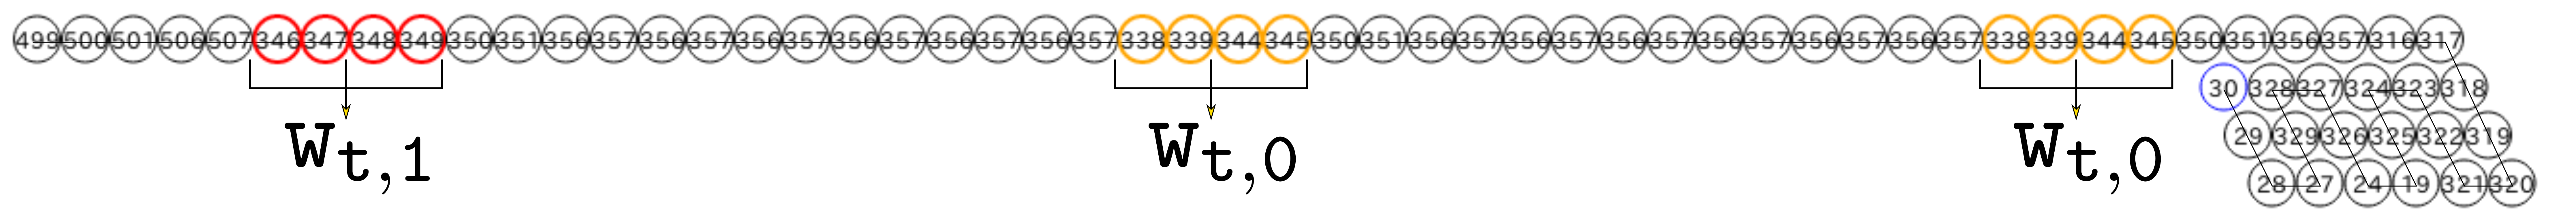
\includegraphics[width=\linewidth]{seed_sample2.png}
\caption{The seed for the 3-bit Heighway dragon that starts at $i = {100}_2$ .}
\end{figure}
\end{frame}

%%%%%%%%%%%%%%%%%%%%%%%%%%%%%%%%%%%%%%%%%%%%%%%%%%%%%%%%%%%%%%%%%%%
\begin{frame}\frametitle{Implementation}\framesubtitle{Information flow}

\centering
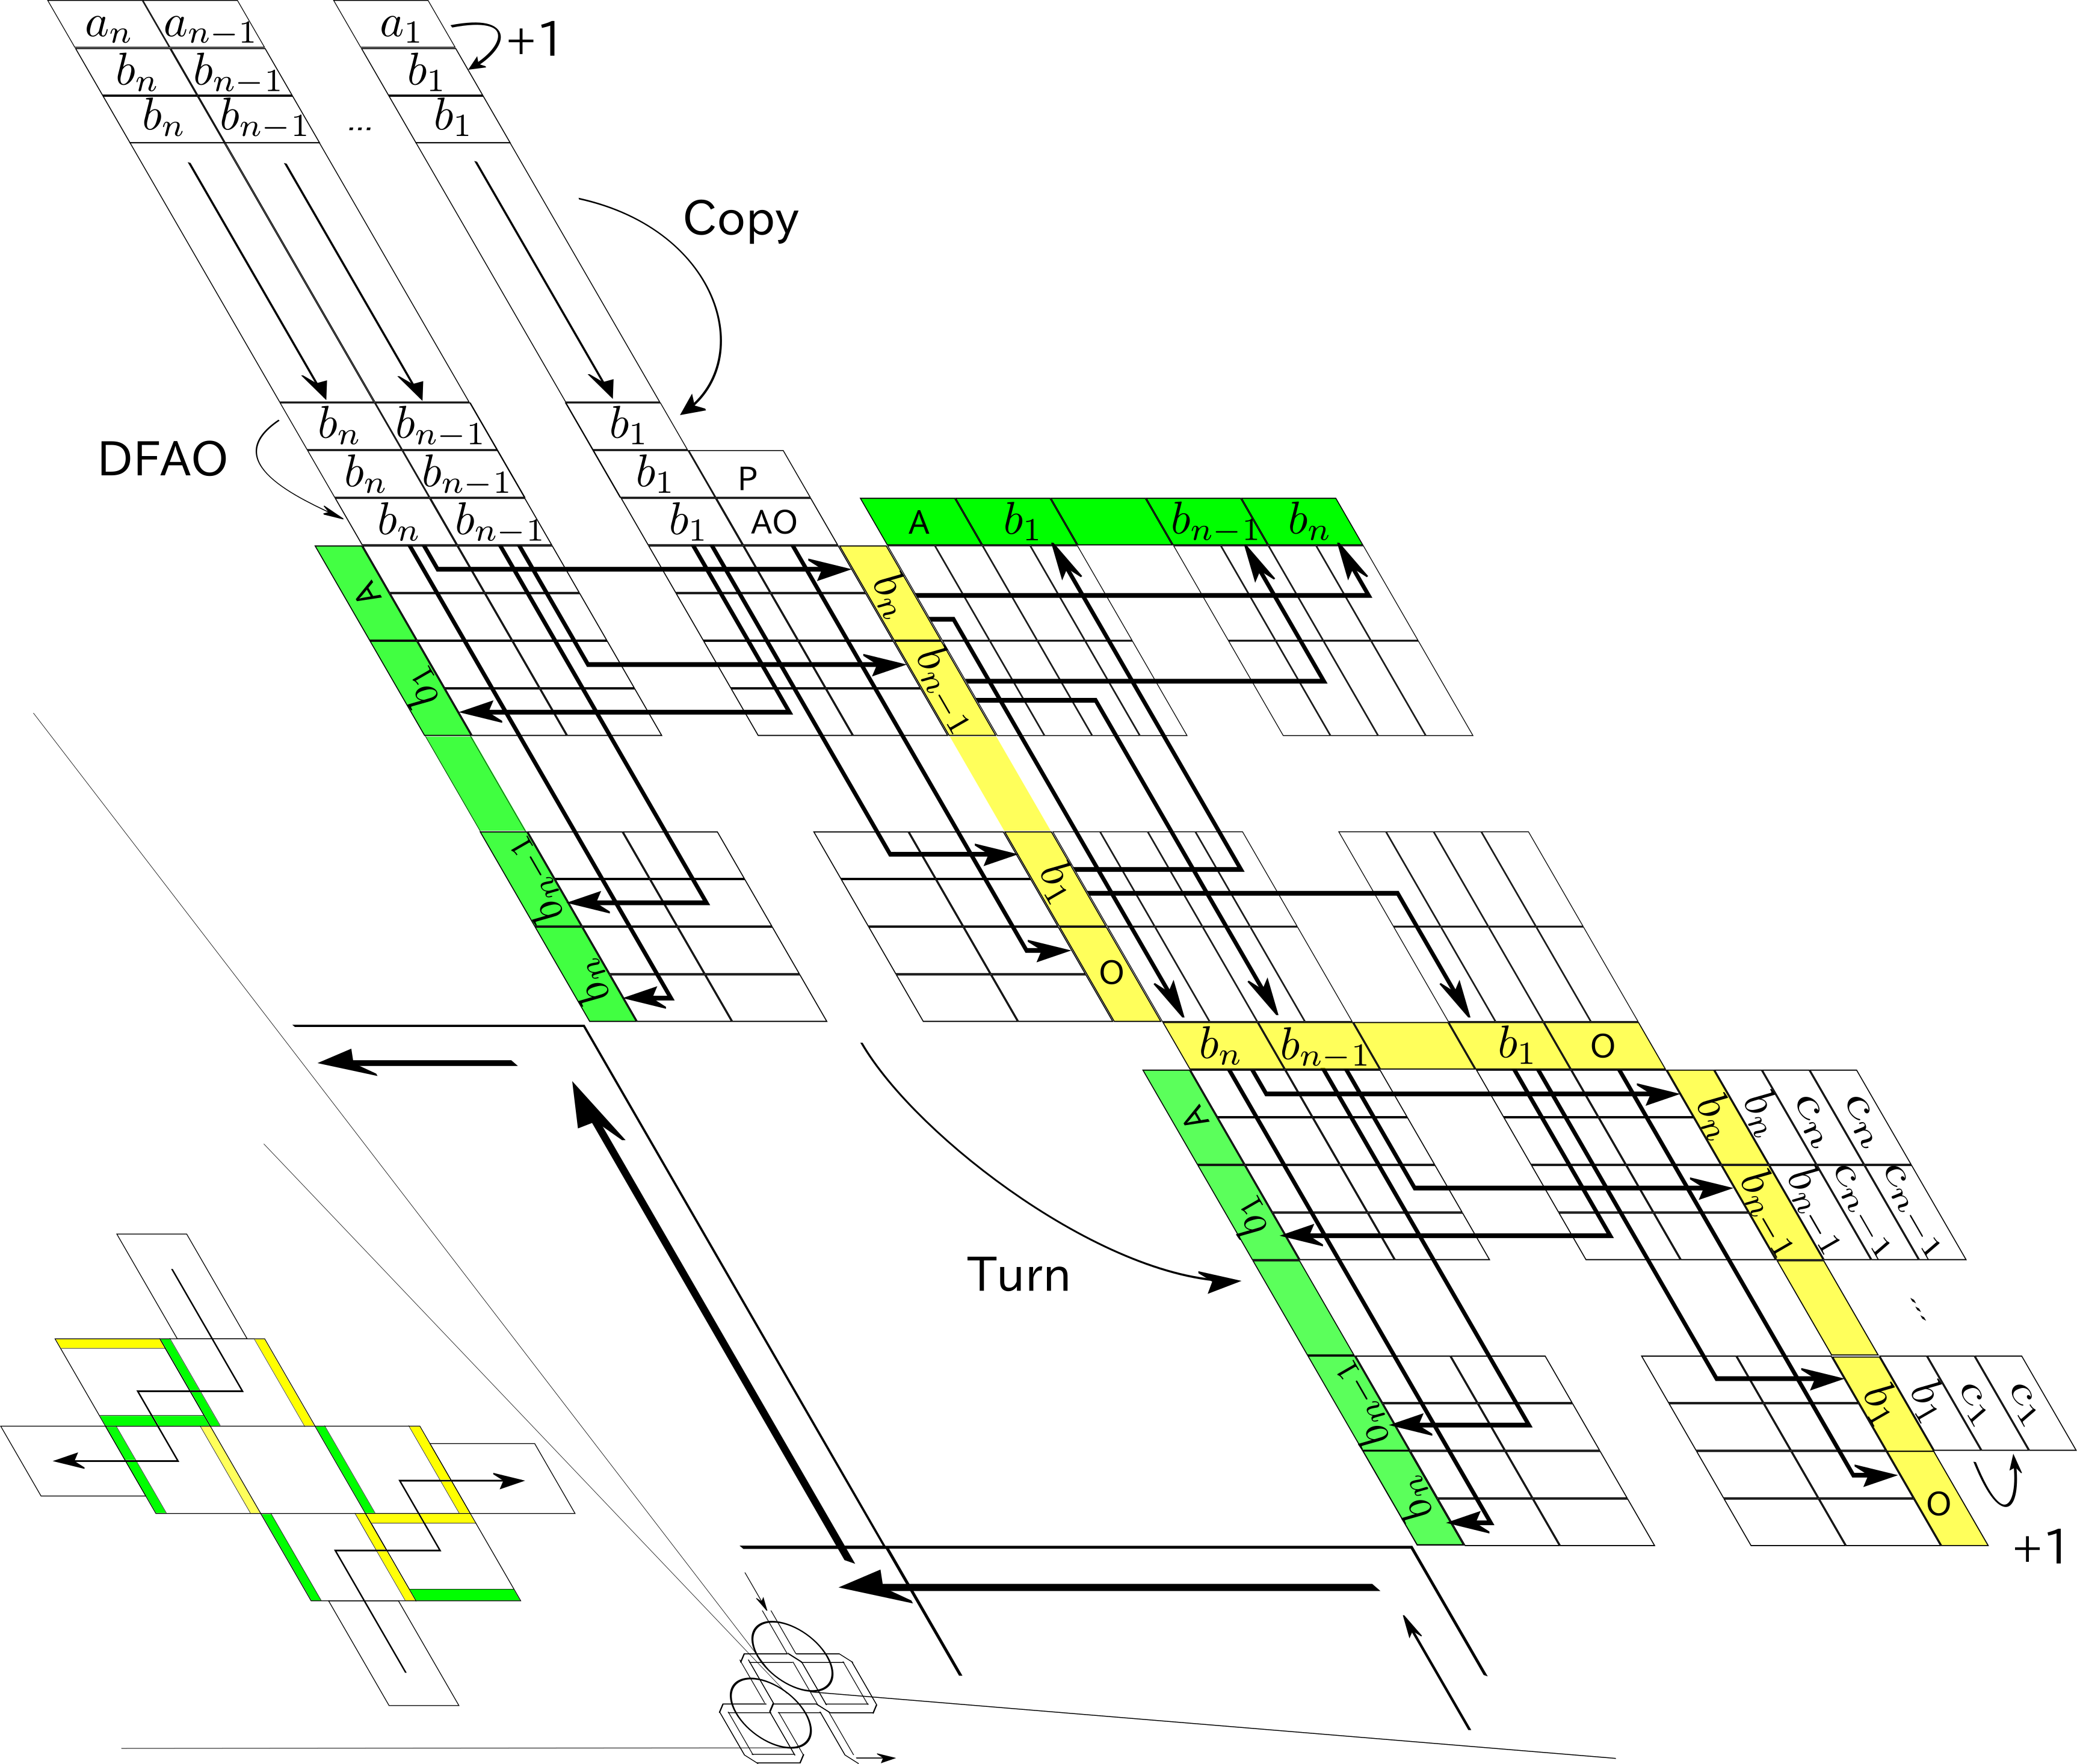
\includegraphics[width=0.6\linewidth]{dragon_vol5.png}

\end{frame}
%%%%%%%%%%%%%%%%%%%%%%%%%%%%%%%%%%%%%%%%%%%%%%%%%%%%%%%%%%%%%%%%%%%

\begin{frame}\frametitle{Implementation}\framesubtitle{DFAO module}

\centering
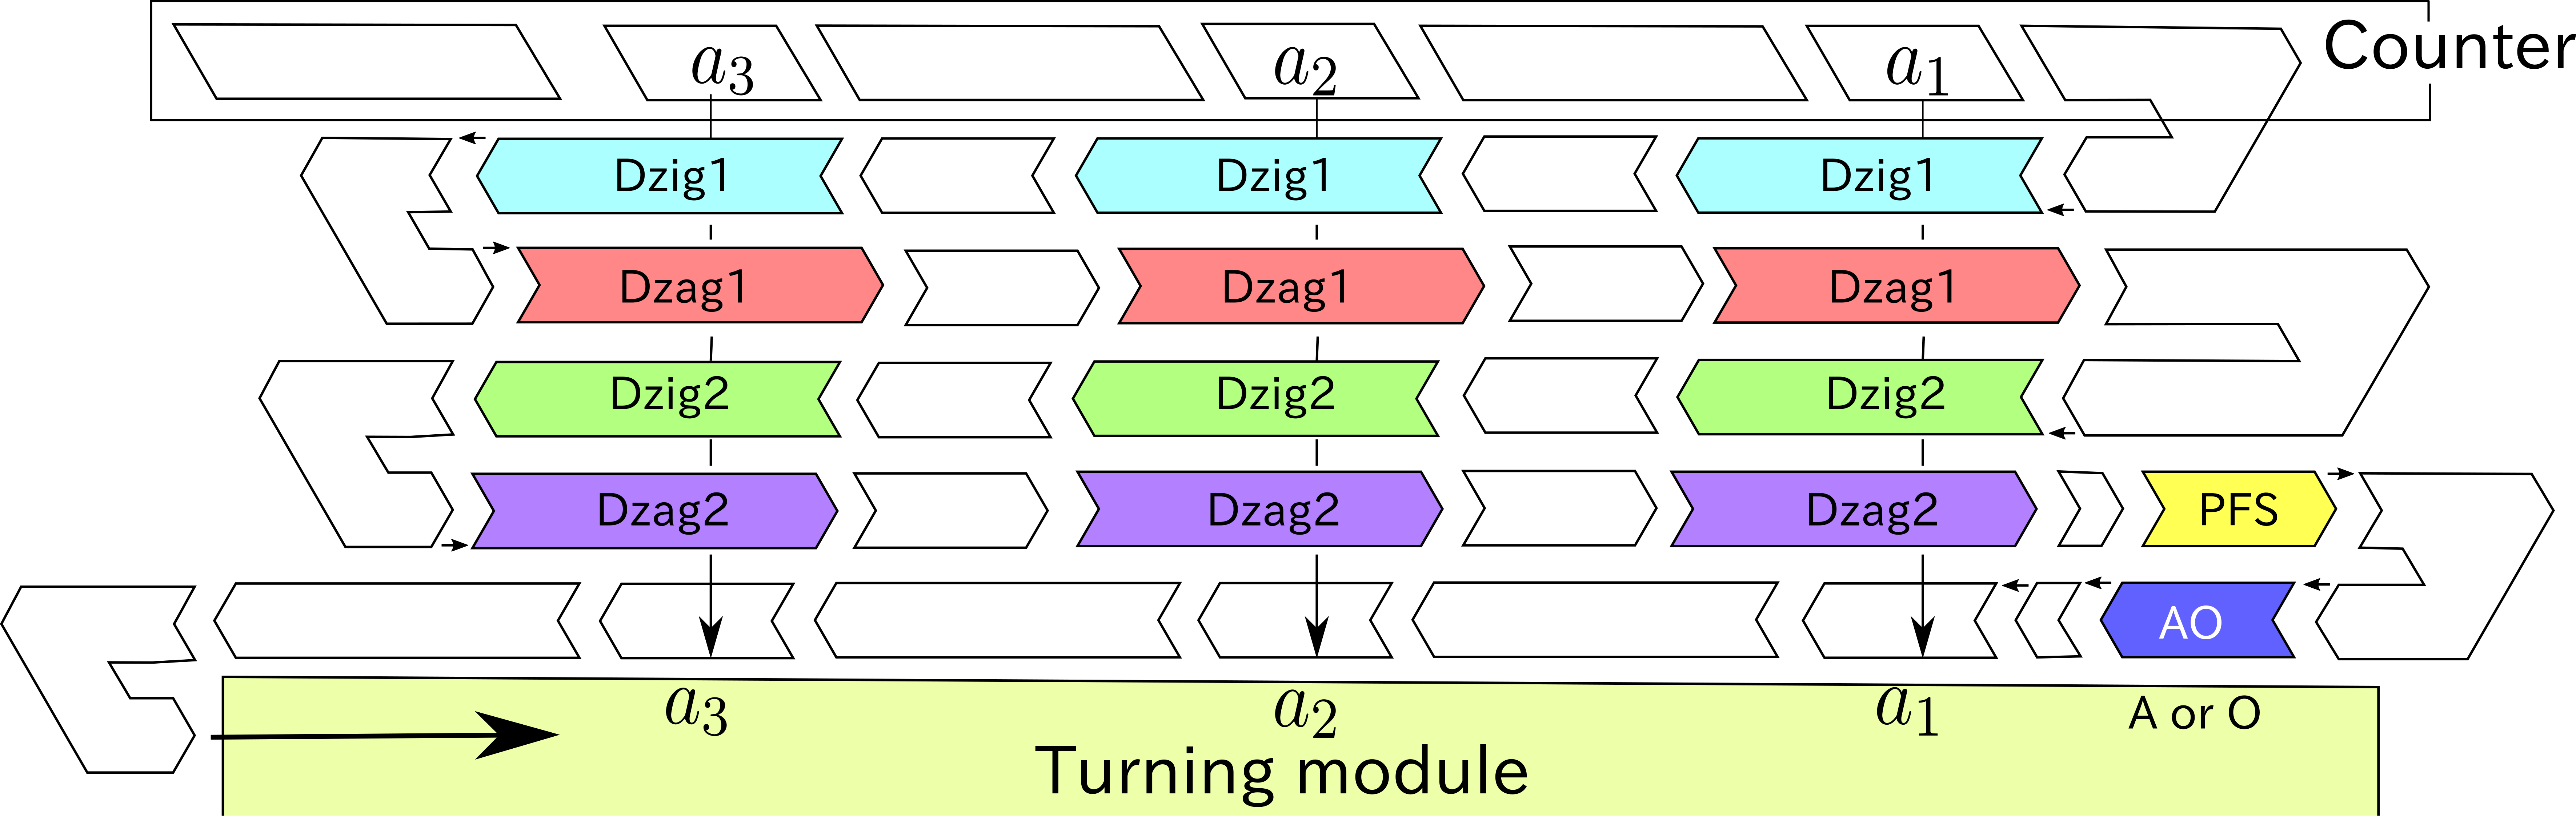
\includegraphics[width=0.7\linewidth]{abst_DFAO.png}

\vspace*{3mm}

\begin{minipage}{0.4\linewidth}
{\footnotesize \begin{itemize}
\item 1st zigzag (Dzig1 \&Dzag1) searches the first 0 (from LSB) and mark it as f0. 
\item 2nd zigzag (Dzig2 \& Dzag2) checks if the f0 is followed by 0 or 1. 
\end{itemize}}

\end{minipage}
\begin{minipage}{0.05\linewidth}
\ \\
\end{minipage}
\begin{minipage}{0.5\linewidth}
\centering
\begin{overlayarea}{\linewidth}{30mm}
\only<1>{
\scalebox{0.7}{\begin{tikzpicture}[>=latex, node distance=2cm, initial text=, bend angle=15]
	\tikzstyle{every initial by arrow} = [->, double];

	\node [state, initial] (q_0)                        {$q_0/R$};
	\node [state]                     (q_1) [right of = q_0]  {$q_1/R$};
	\node [state]                     (q_2) [below right of = q_1] {$q_2/L$};
	\node [state]                     (q_3) [above right of = q_1] {$q_3/R$};

	\path [->] (q_0) edge [right] node [above]              {$0$}                 (q_1)
         		         edge [loop above] node [above]             {$1$}               ()
         			   (q_1) edge [bend left] node [above]             {$0$}                 (q_3)
         		         edge [bend right] node [below]             {$1$}              (q_2)
         			   (q_2)  edge [loop right] node [above]             {$0,1$}               ()
         			   (q_3)  edge [loop right] node [above]             {$0,1$}               ();
\end{tikzpicture}}
}
\end{overlayarea}
\end{minipage}
\end{frame}

%%%%%%%%%%%%%%%%%%%%%%%%%%%%%%%%%%%%%%%%%%%%%%%%%%%%%%%%%%%%%%%%%%
\begin{frame}
\frametitle{Implementation}
\framesubtitle{DFAO module}

\large{
\only<1-9>{Current count = 101}
\only<10>{Current count = 100}
}
\begin{figure}[H]
  	\centering
	\only<1>{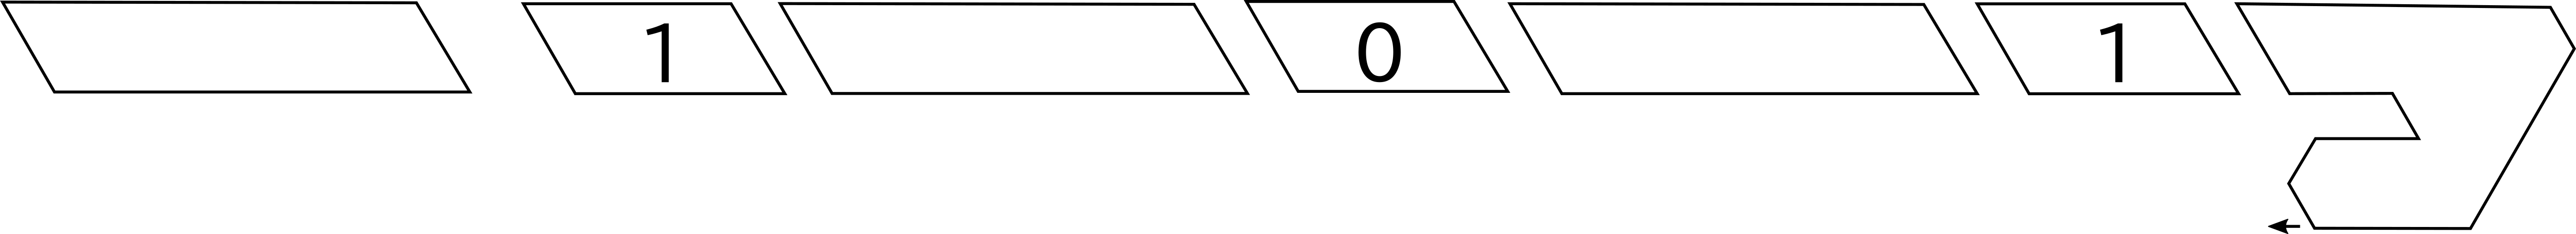
\includegraphics[width=\linewidth]{example_DFAO1.png}}
	\only<2>{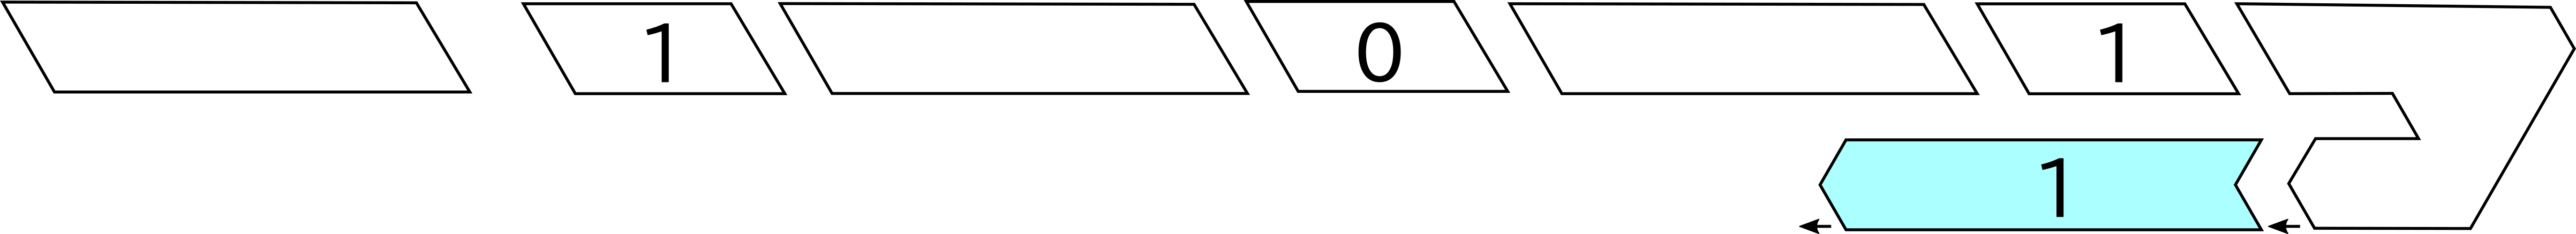
\includegraphics[width=\linewidth]{example_DFAO2.png}}
	\only<3>{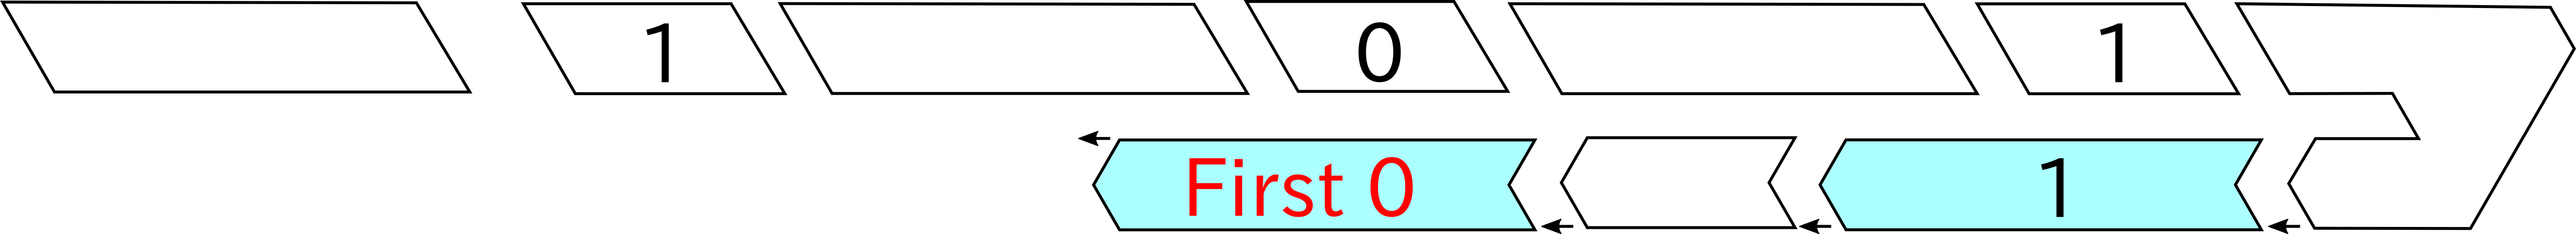
\includegraphics[width=\linewidth]{example_DFAO3.png}}
	\only<4>{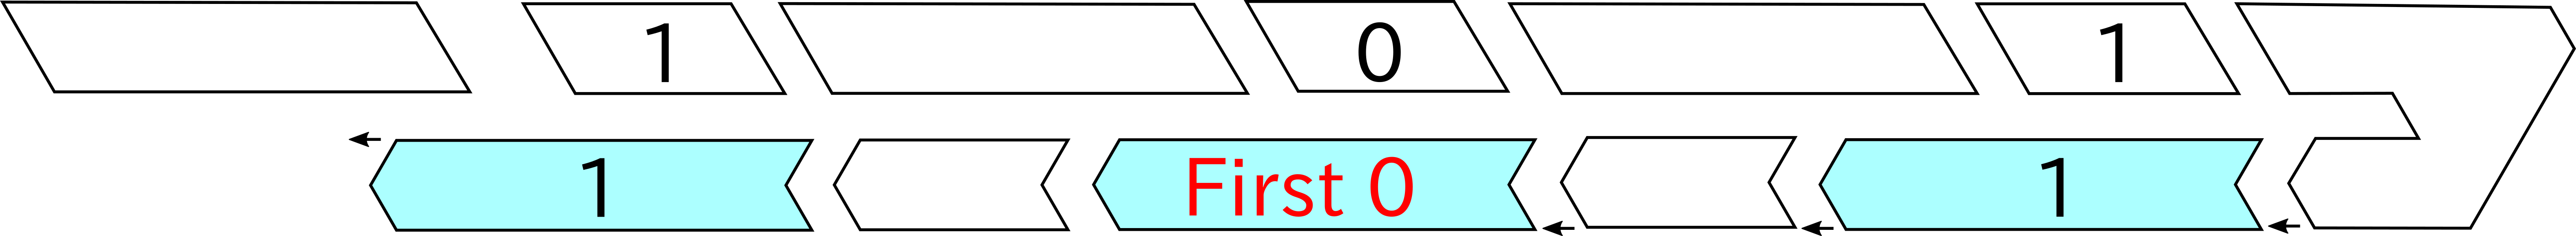
\includegraphics[width=\linewidth]{example_DFAO3_5.png}}
	\only<5>{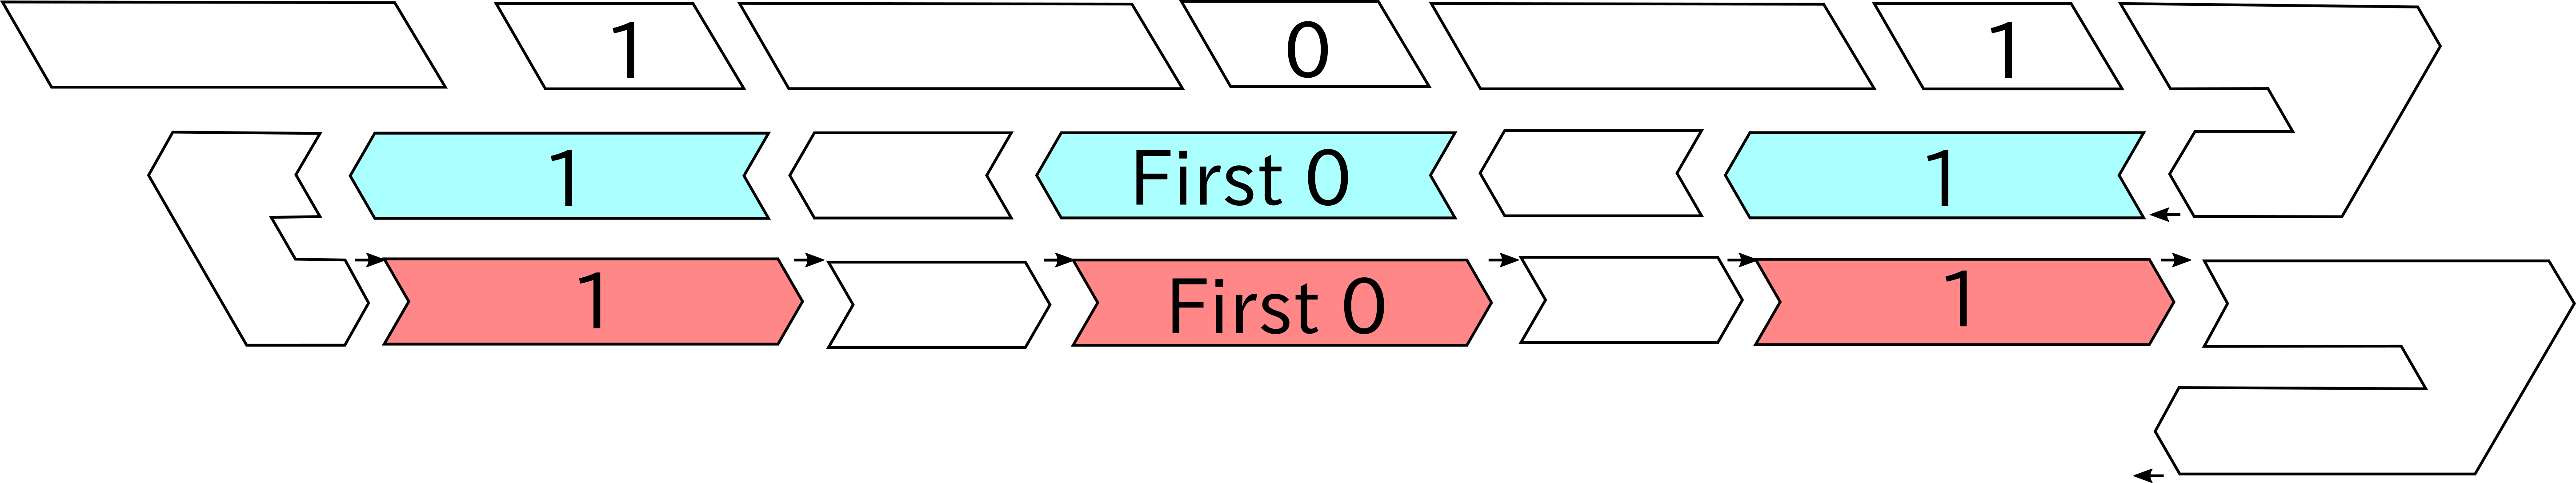
\includegraphics[width=\linewidth]{example_DFAO3_75.png}}
	\only<6>{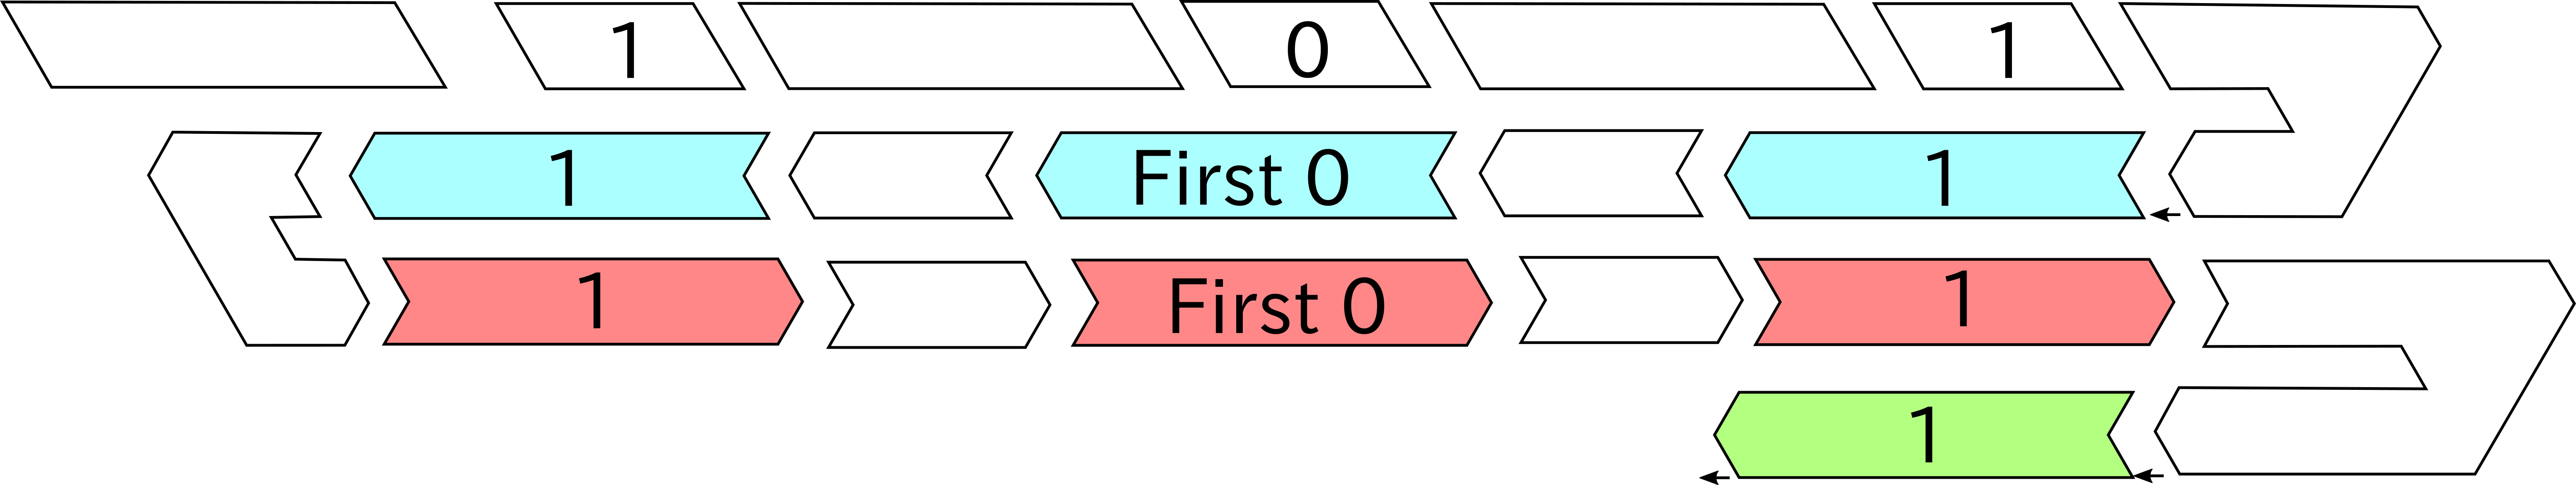
\includegraphics[width=\linewidth]{example_DFAO4.png}}
	\only<7>{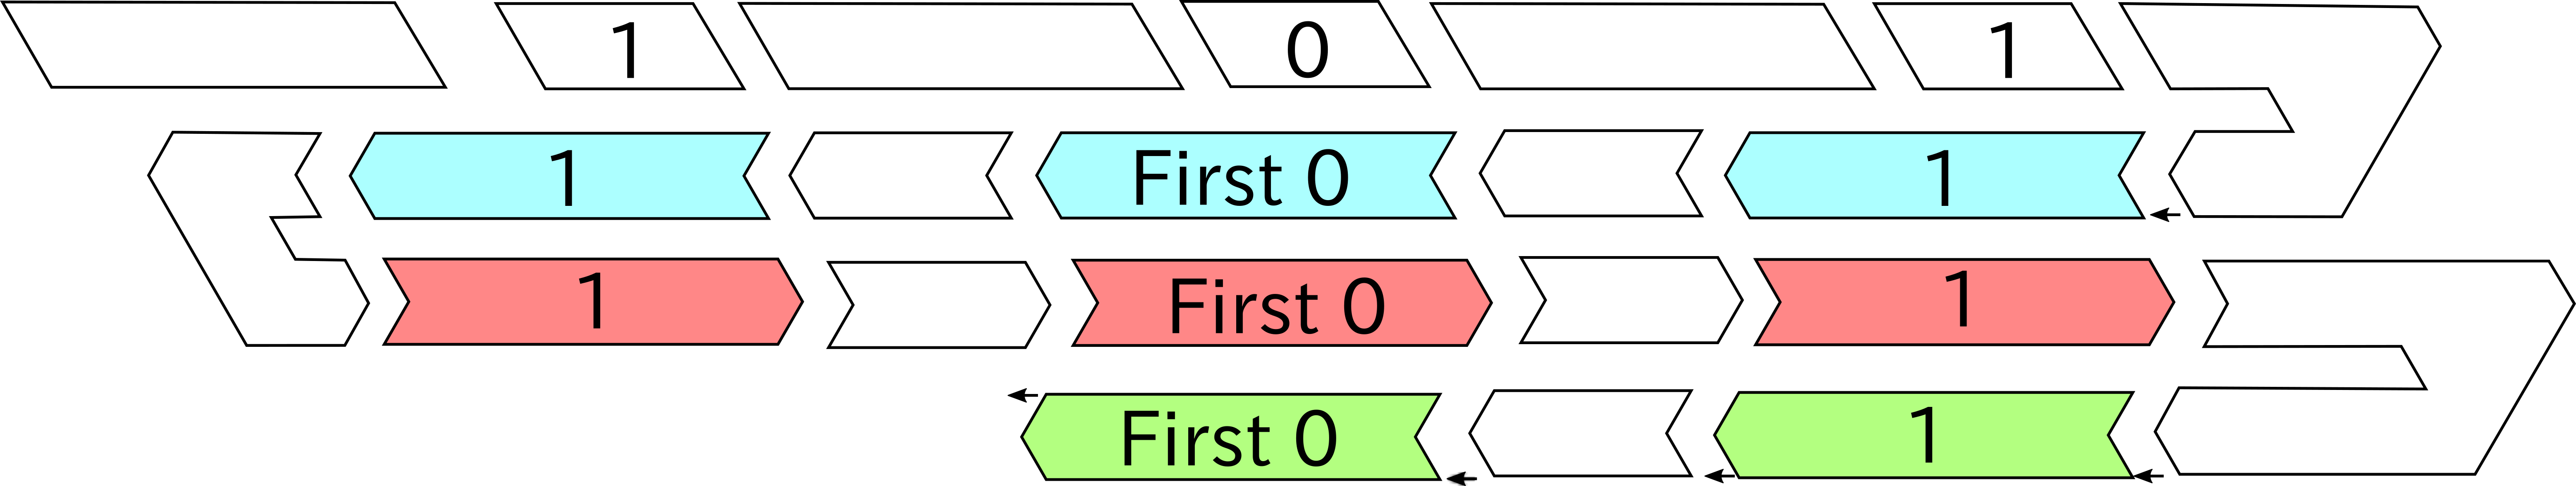
\includegraphics[width=\linewidth]{example_DFAO5.png}}
	\only<8>{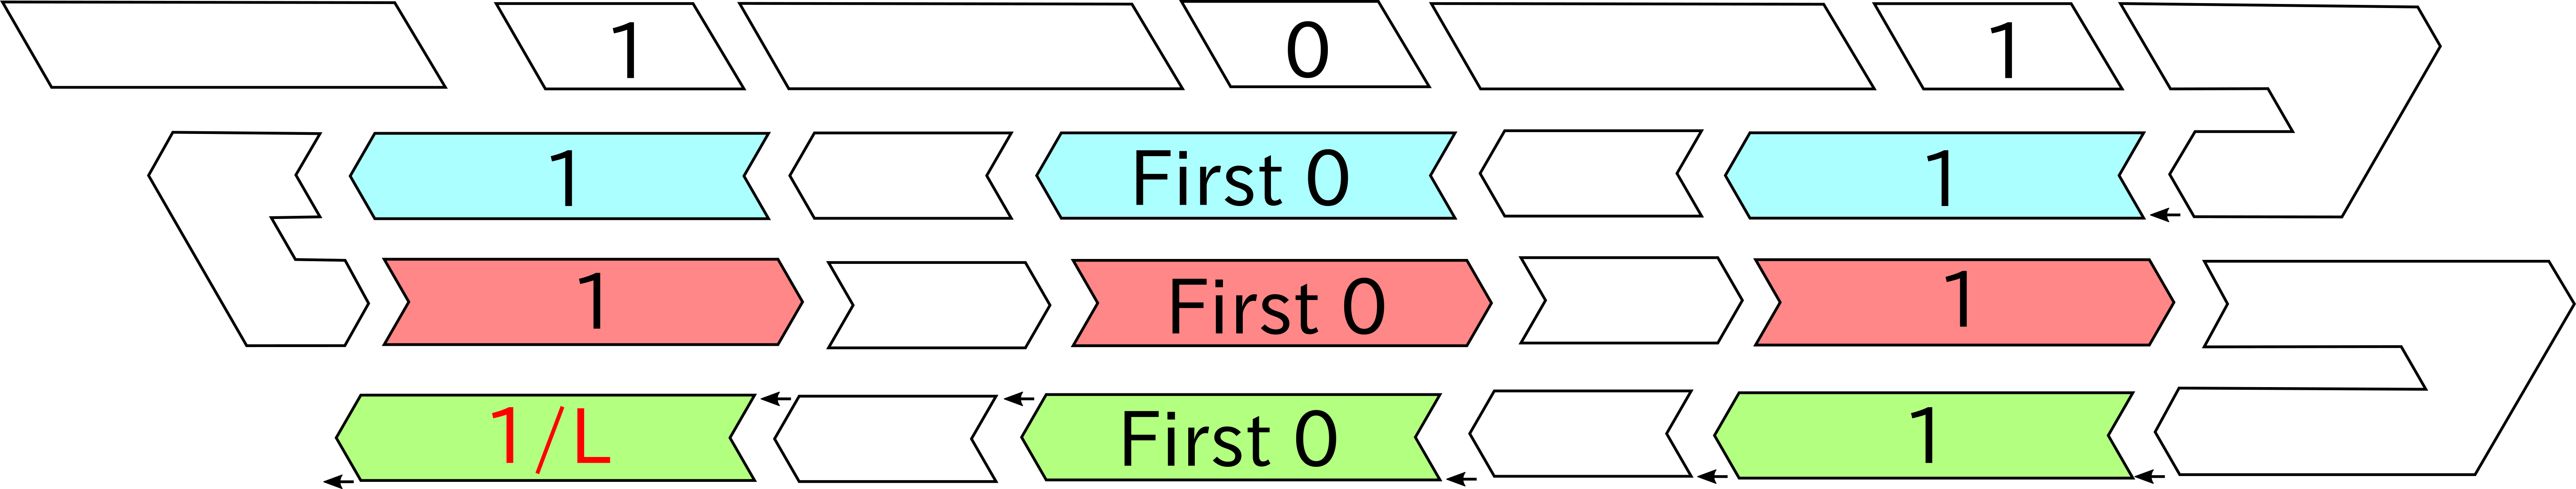
\includegraphics[width=\linewidth]{example_DFAO6.png}}
	\only<9>{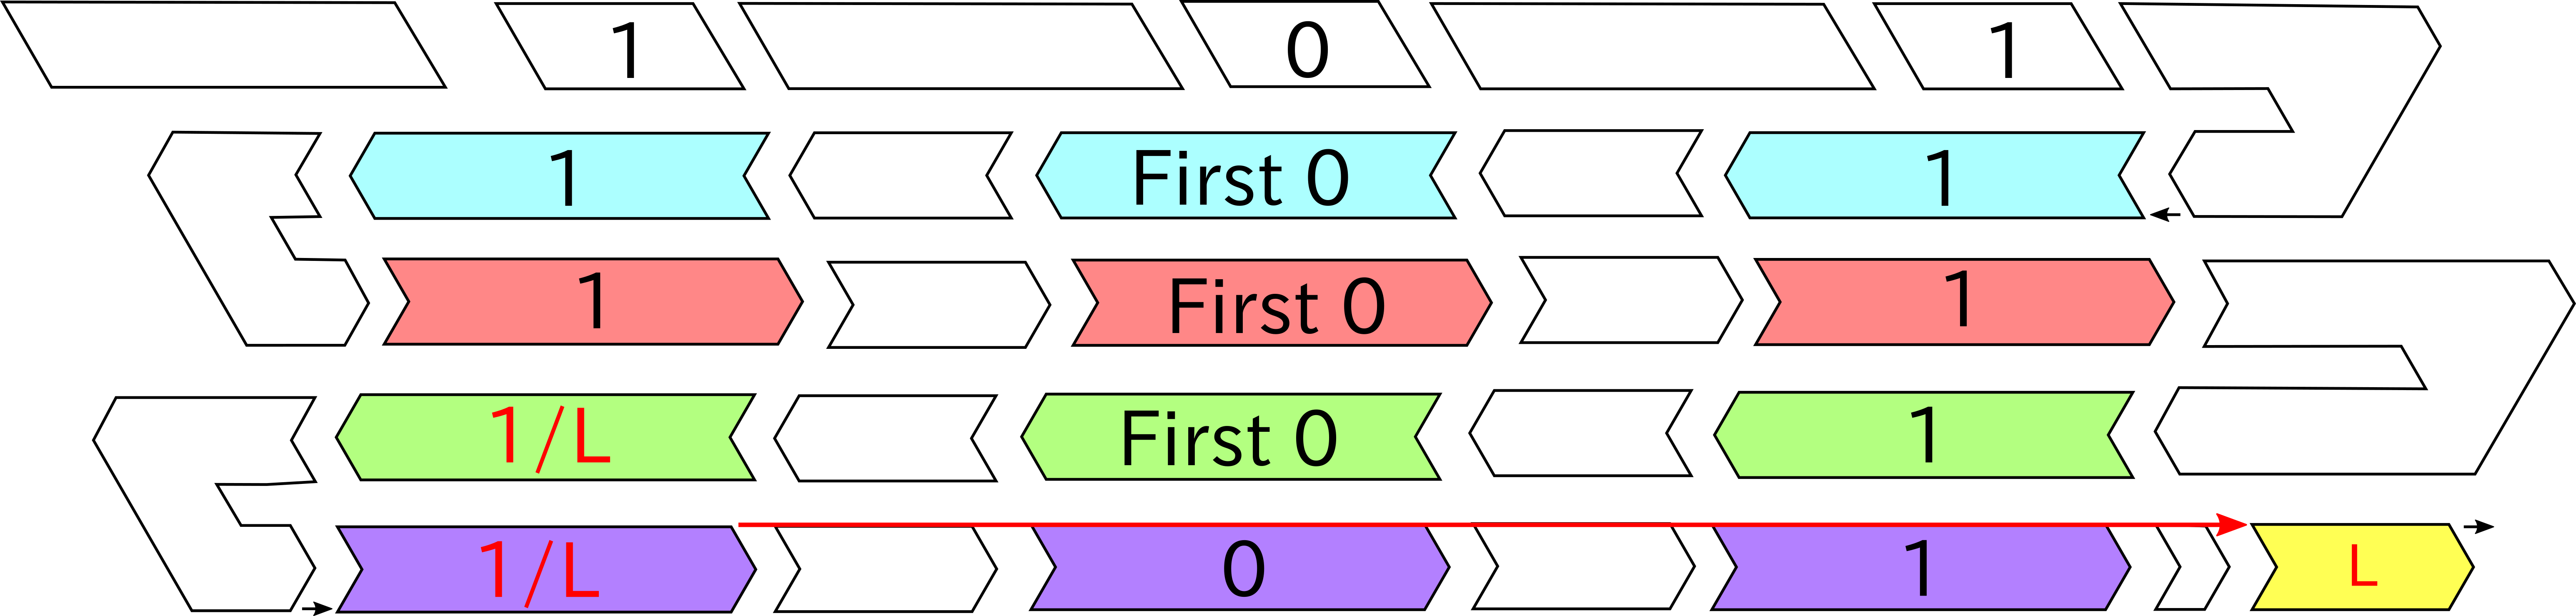
\includegraphics[width=\linewidth]{example_DFAO7.png}}
	\only<10>{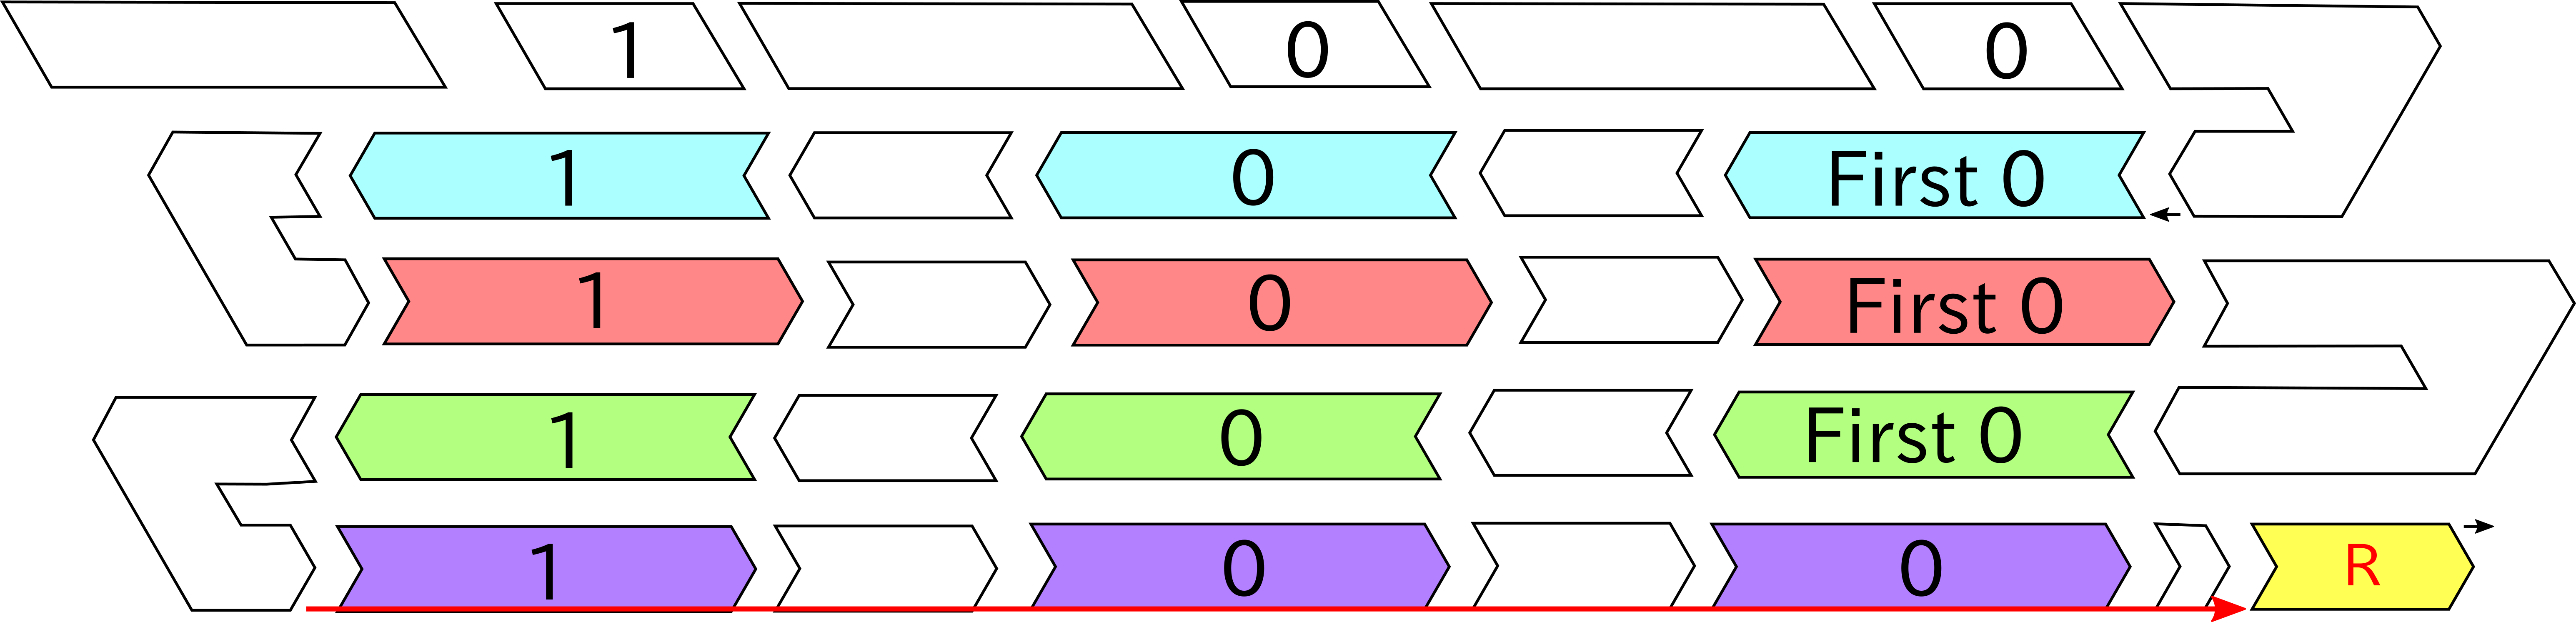
\includegraphics[width=\linewidth]{example_DFAO8.png}}
\end{figure}
\begin{center}
\scalebox{0.7}{\begin{tikzpicture}[>=latex, node distance=2.2cm, initial text=, bend angle=15]
	\tikzstyle{every initial by arrow} = [->, double];

	\node [state, initial] (q_0)                        {$q_0/R$};
	\node [state]                     (q_1) [right of = q_0]  {$q_1/R$};
	\uncover<3-7>{\node [state,red]                     (q_1) [right of = q_0]  {$q_1/R$};}
	\node [state]                     (q_2) [below right of = q_1] {$q_2/L$};
	\node [state]                     (q_3) [above right of = q_1] {$q_3/R$};
	\uncover<10>{\node [state, red]                     (q_3) [above right of = q_1] {$q_3/R$};}
	\uncover<8-9>{\node [state,red]                     (q_2) [below right of = q_1] {$q_2/L$};}

	\path [->] (q_0) edge [right] node [above]              {$0$}                 (q_1)
         		         edge [loop above] node [above]             {$1$}               ()
         			   (q_1) edge [bend left] node [above]             {$0$}                 (q_3)
         		         edge [bend right] node [below]             {$1$}              (q_2)
         			   (q_2)  edge [loop right] node [above]             {$0,1$}               ()
         			   (q_3)  edge [loop right] node [above]             {$0,1$}               ();
\end{tikzpicture}
}
\end{center}
\end{frame}


%%%%%%%%%%%%%%%%%%%%%%%%%%%%%%%%%%%%%%%%%%%%%%%%%%%%%%%%%%%%%%%%%%
\begin{frame}
\frametitle{Implementation}
\framesubtitle{Turning module}

\centering
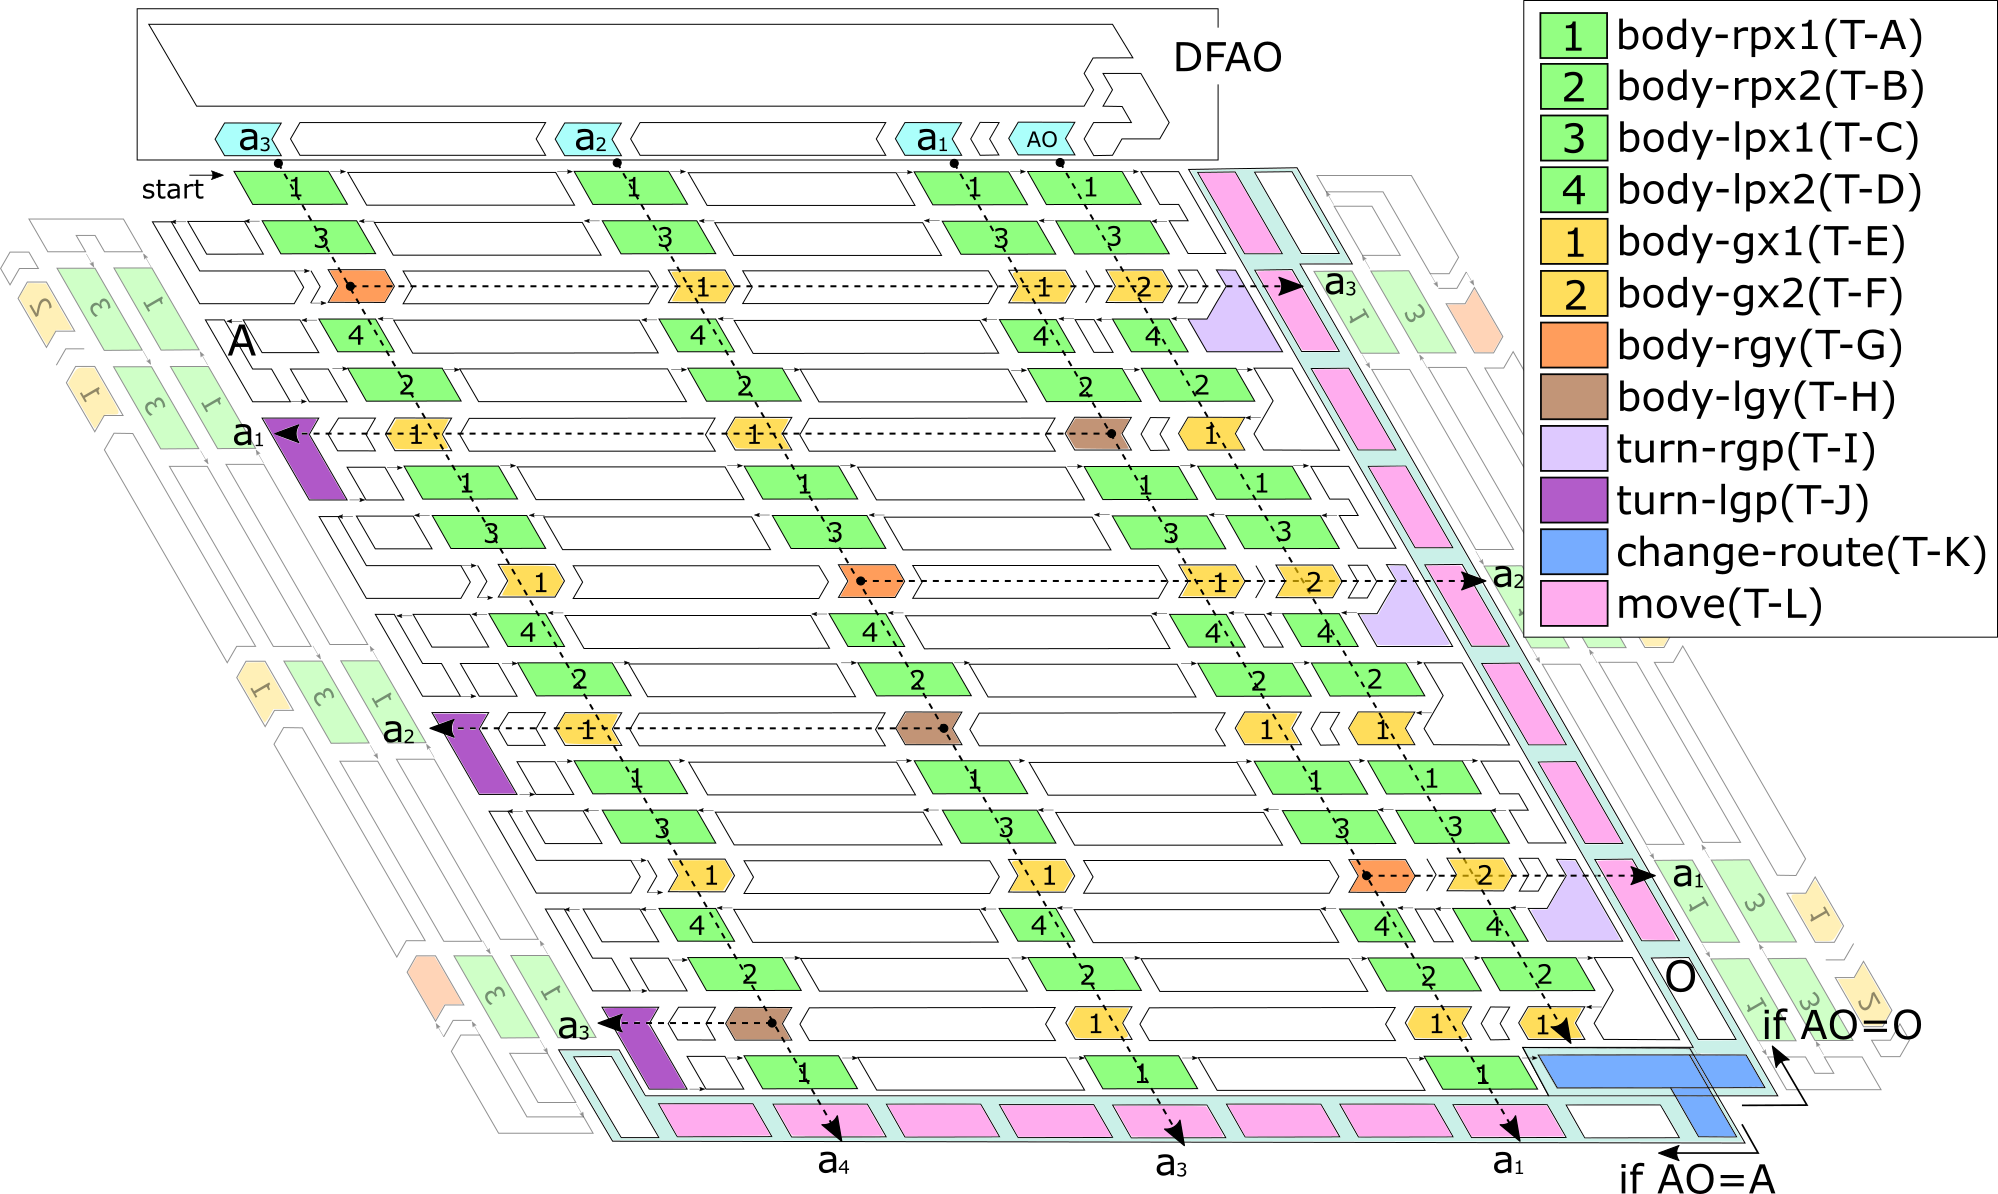
\includegraphics[width=\linewidth]{overall_turn_part.png}

\end{frame}

%%%%%%%%%%%%%%%%%%%%%%%%%%%%%%%%%%%%%%%%%%%%%%%%%%%%%%%%%%%%%%%%%%%
\begin{frame}
\frametitle{Implementation}


\begin{alertblock}{Brick automata}
\centering
\includegraphics[width=\linewidth-1.5cm]{D-zig1_brick.png}
\end{alertblock}

\end{frame}
%%%%%%%%%%%%%%%%%%%%%%%%%%%%%%%%%%%%%%%%%%%%%%%%%%%%%%%%%%%%%%%%%%

\begin{frame}
\frametitle{Implementation}
\framesubtitle{Result}

\centering
\href{run:dragon.mp4}{
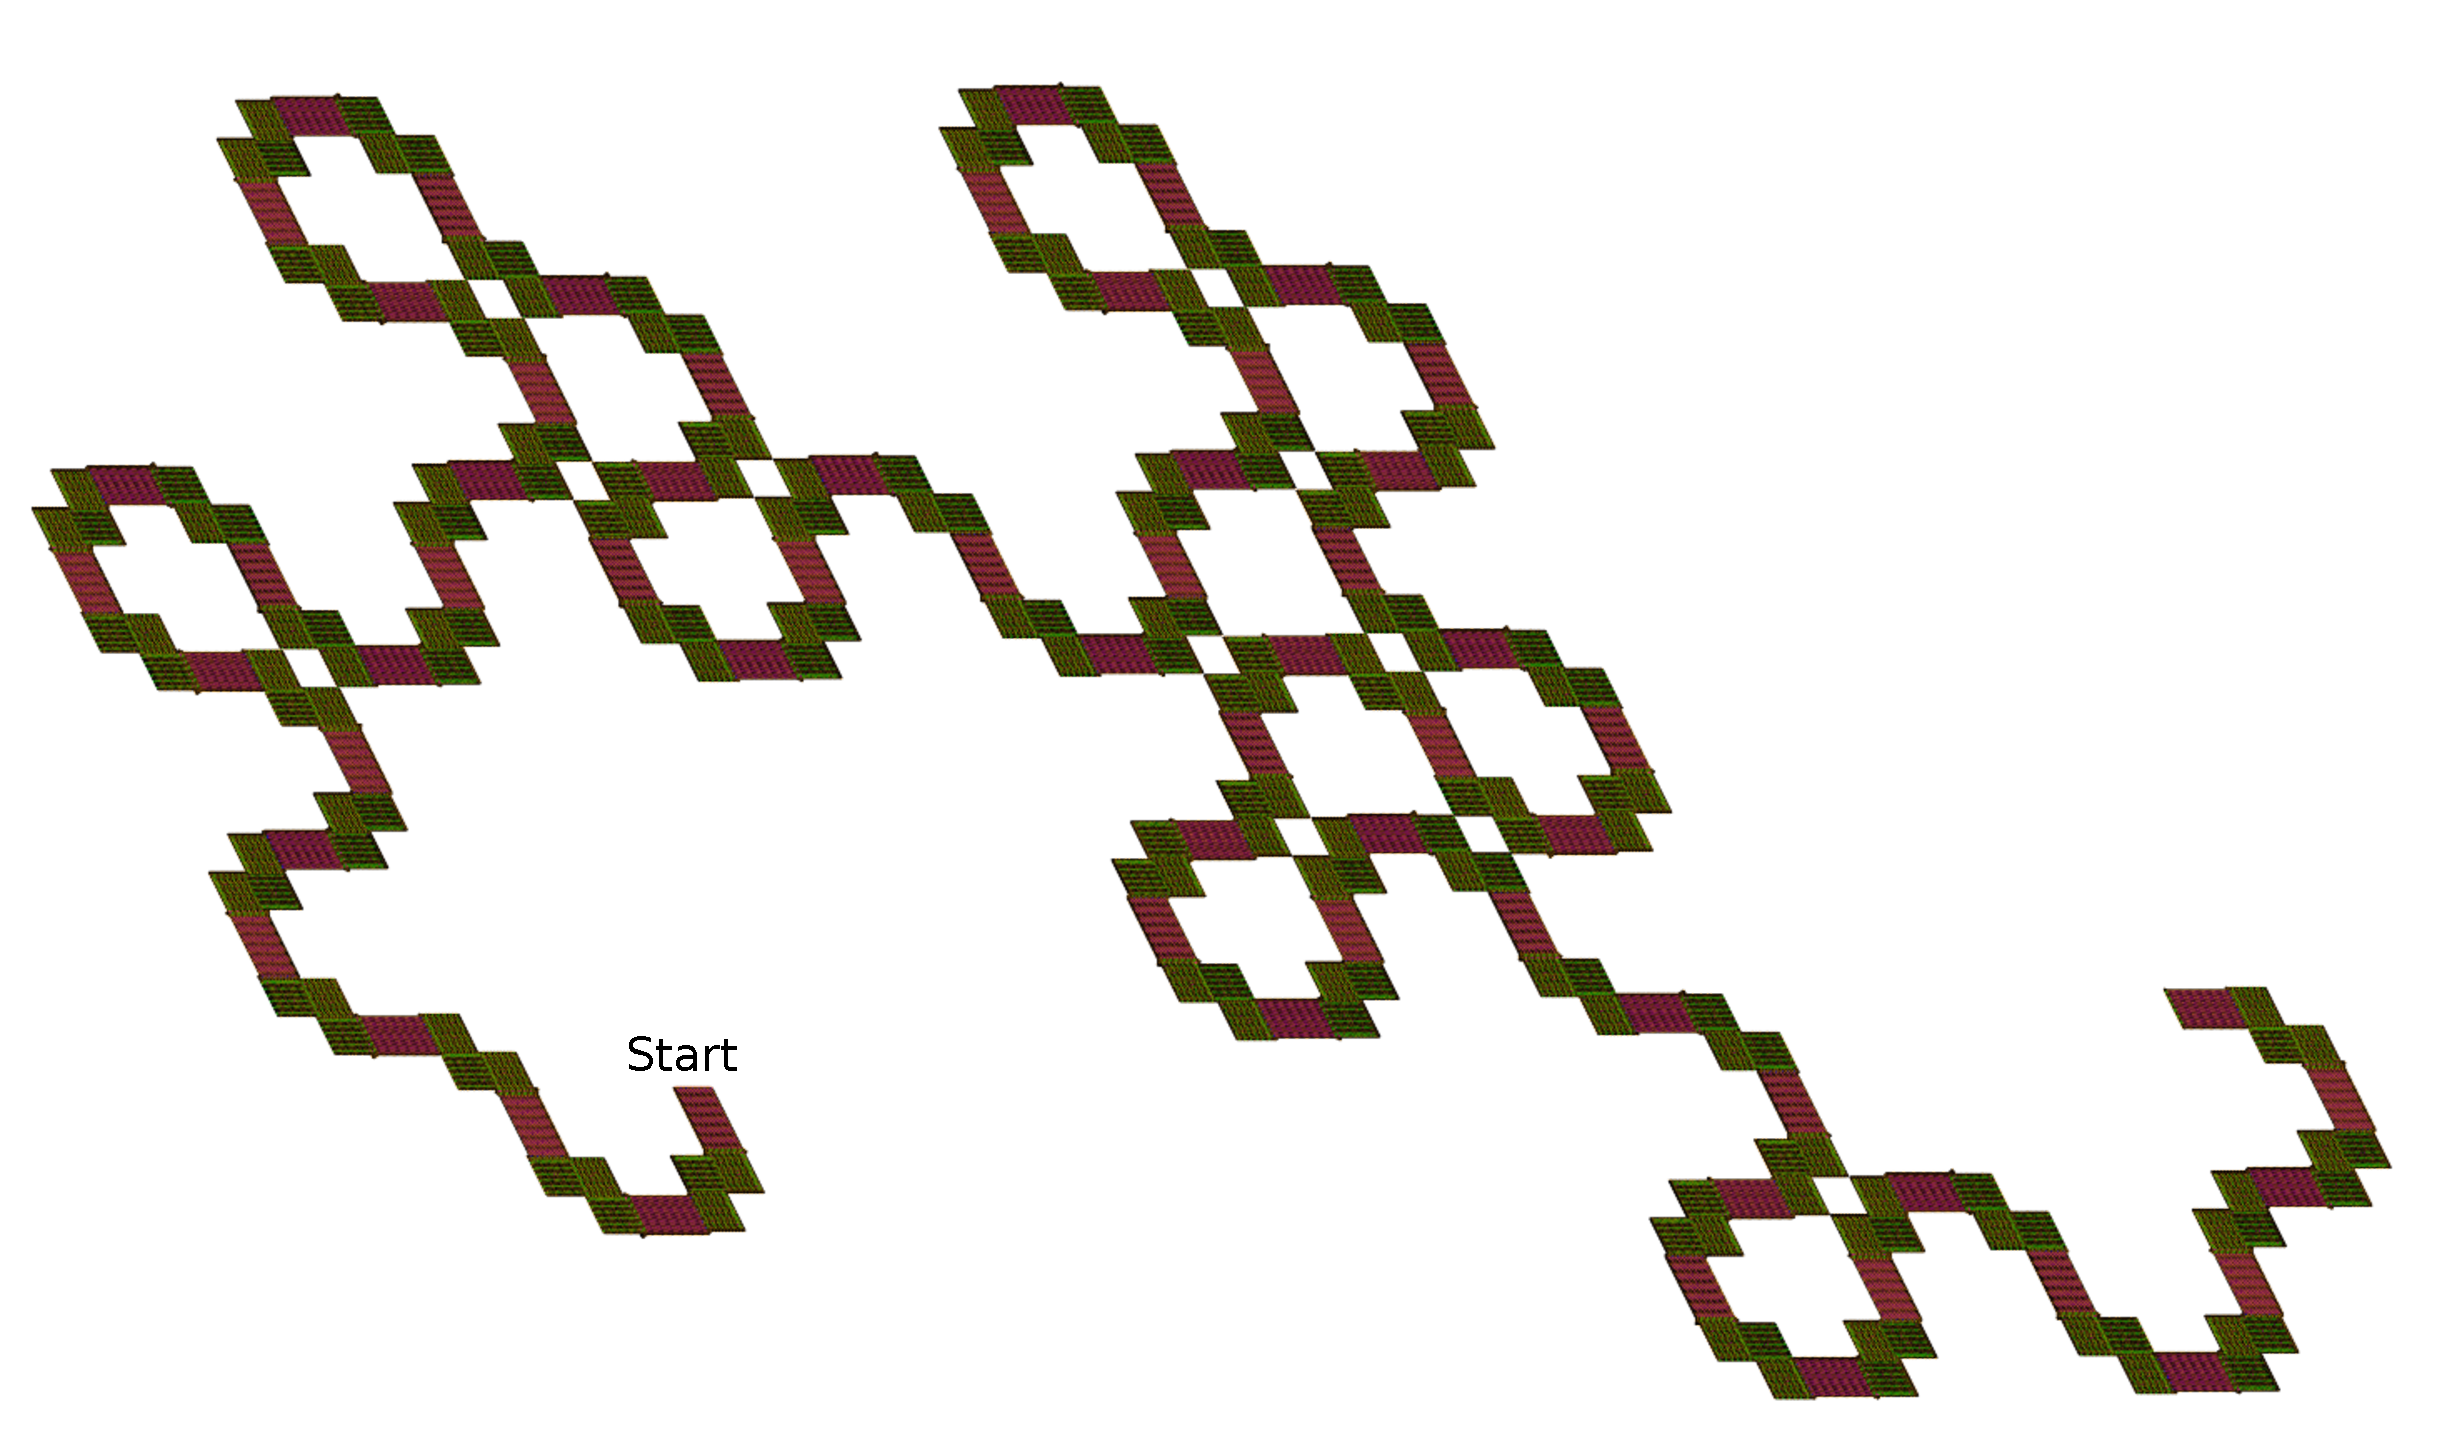
\includegraphics[width=\linewidth]{6bit_heighway.pdf}
}
\end{frame}
%%%%%%%%%%%%%%%%%%%%%%%%%%%%%%%%%%%%%%%%%%%%%%%%%%%%%%%%%%%%%%%%%%
\section{ }

\frame{
\frametitle{Acknowledgements}

\begin{center}
{\Large Thanks a lot for your attention!!}
\end{center}

{\scriptsize
Supported in part by %\hspace*{3cm}
\begin{itemize}
%\item Academy of Finland, Postdoctoral Researcher Grant 13266670/T30606
\item JSPS KAKENHI Grant-in-Aid for Young Scientists (A) 16H05854 
\item JSPS KAKENHI Grant-in-Aid for Challenging Research (Exploratory) 18K19779
\item JSPS and NRF under the Japan-Korea Basic Scientific Cooperation Program YB29004.
\end{itemize}
}

\vspace*{5mm}

\centering

\begin{minipage}{0.3\linewidth}
\centering

\includegraphics[width=0.75\linewidth]{KAKENHIlogo.jpg}
\end{minipage}
\begin{minipage}{0.01\linewidth}
\ \\
\end{minipage}
\begin{minipage}{0.3\linewidth}
\centering

\includegraphics[width=1.1\linewidth]{nihongakuzyutu.jpg}
\end{minipage}
\begin{minipage}{0.01\linewidth}
\ \\
\end{minipage}
\begin{minipage}{0.3\linewidth}
\centering

\includegraphics[width=0.6\linewidth]{logo_nrf.jpg}
\end{minipage}
}

%%%%%%%%%%%%%%%%%%%%%%%%%%%%%%%%%%%%%%%%%%%%%%%%%%%%%%%%%%%%%%%%%%


\frame{
\frametitle{Acknowledgements}

\begin{center}
{\Large Thanks a lot for your attention!!}
\end{center}
\begin{columns}
\begin{column}{3cm}
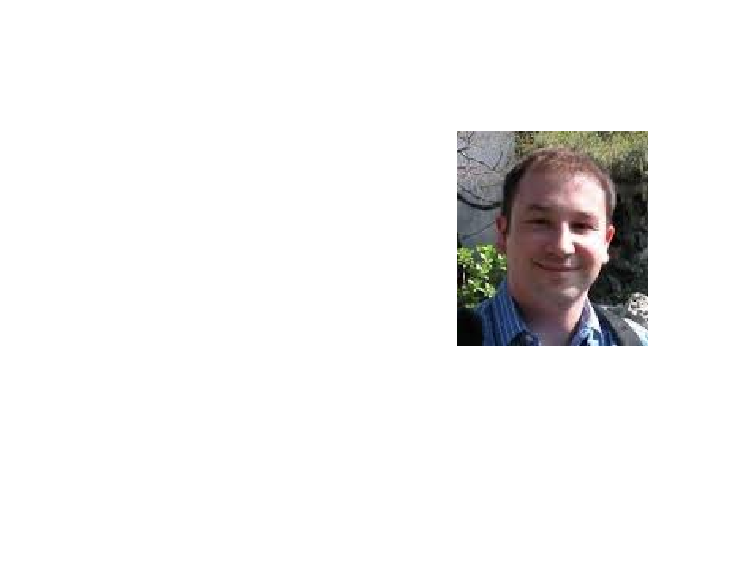
\includegraphics[width=2.5cm]{nicolas.pdf}\\
Nicolas Schabanel
(LIAFA, ENS de Lyon)
\vspace{2cm} 
\end{column}
\begin{column}{3cm}
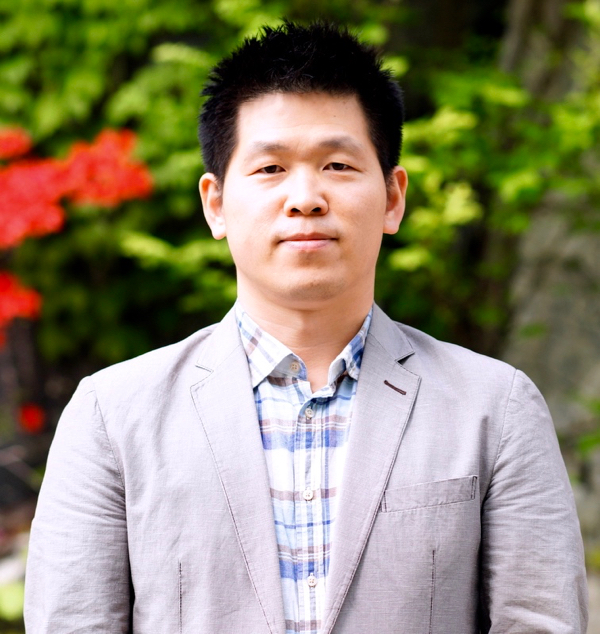
\includegraphics[width=2.5cm]{yo-sub.jpg}\\
Yo-Sub Han
(Yonsei Univ.)
\vspace{2cm} 
\end{column}
\begin{column}{3cm}

\includegraphics[width=2.5cm]{hwee.jpg}\\
Hwee Kim
(Univ. of South Florida)
\vspace{2cm} 
\end{column}
\end{columns}
}
%%%%%%%%%%%%%%%%%%%%%%%%%%%%%%%%%%%%%%%%%%%%%%%%%%%%%%%%%%%%%%%%%%%%





\frame[allowframebreaks]{
\frametitle{References}


\begin{thebibliography}{1}

%\bibitem[Arkin2009]{Arkin2009}
%	E. M. Arkin, S. P. Fekete, I. Kamrul, H. Meijer, J. S. B. Mitchell, Y. N. nez Rodriguez, V. Polishchuk, D. Rappaport, and H. Xiao
%	\newblock Not being (super)thin or solid is hard: A study of grid Hamiltonicity, 
%	\newblock {\em Computational Geometry: Theory and Applications} 42(6-7) (2009) 582-605
%
%\bibitem[Feynman 1996]{Feynman1996}
%	R. P. Feynman 
%	\newblock Feynman Lectures on Computation. 
%	\newblock Perseus (for Hbg), 1996
	
\bibitem[Geary et al. 2016]{GeMeScSe2016}
	C. Geary, P-E. Meunier, N. Schabanel, S. Seki 
	\newblock Programming biomolecules that fold greedily during translation. 
	\newblock Proc. MFCS 2016, LIPIcs 58, 43:1-43:14, 2016

\bibitem[Geary, Rothemund, Andersen ,{\it Science} 345 (2014) 799-804]{Geary2014}
	C. Geary, P. W. K. Rothemund, E. S. Andersen 
	\newblock A single-stranded architecture for cotranscriptional folding of RNA nanostructures. 
	\newblock {\it Science} 345 (2014) 799-804
	
	
\bibitem[Watters et al. 2016]{Watters2016}
	K. E. Watters, E. J .Strobel, A. M. Yu, J. T. Lis, and J. B. Lucks
	\newblock Cotranscriptional folding of a riboswitch at nucleotide resolution. 
	\newblock {\it Nat. Struct. Mol. Biol.} 23(12) (2016) 1124-1133

\end{thebibliography}
}
%%%%%%%%%%%%%%%%%%%%%%%%%%%%%%%%%%%%%%%%%%%%%%%%%%%%%%%%%%%%%%%%%%
\frame{
\frametitle{Advertisement 1}

\begin{minipage}{0.45\linewidth}
\centering
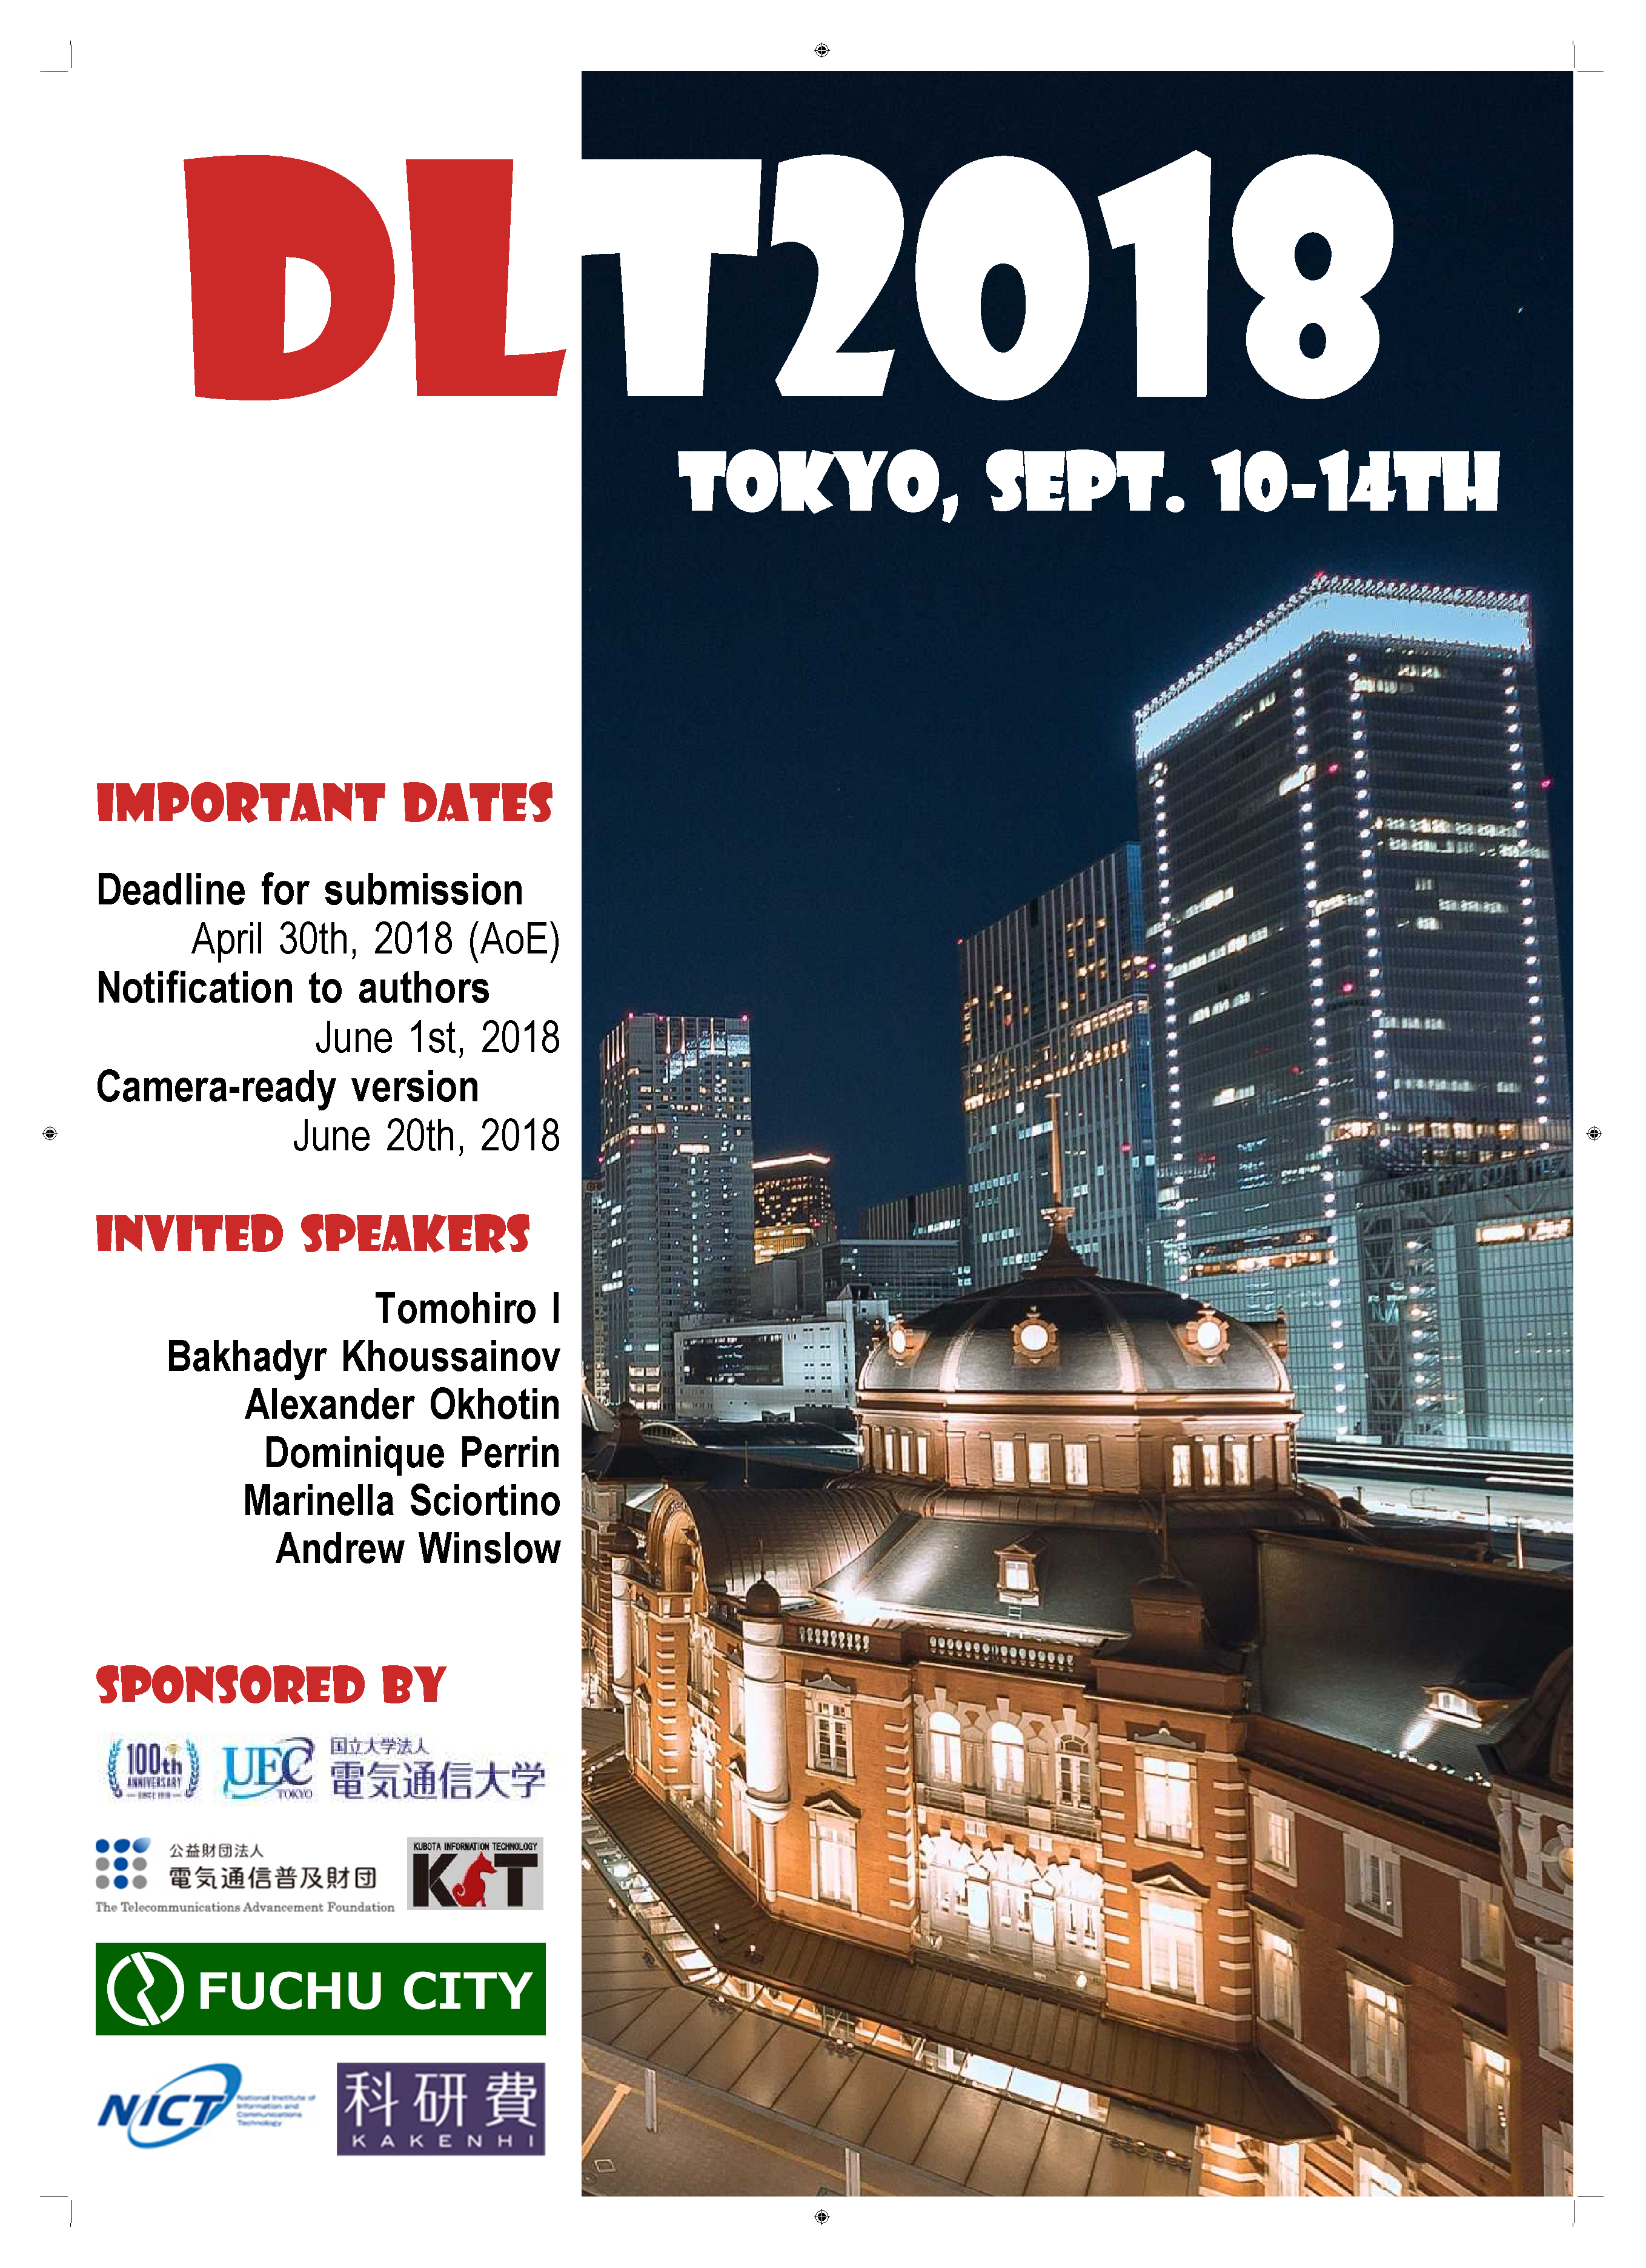
\includegraphics[width=\linewidth]{dlt2018poster.pdf}
\end{minipage}
\begin{minipage}{0.05\linewidth}
\ \\
\end{minipage}
\begin{minipage}{0.45\linewidth}


\href{https://dlt2018.uec.ac.jp}{\textcolor{blue}{https://dlt2018.uec.ac.jp}}

\vspace*{5mm}
{\footnotesize 

\begin{itemize}
\item Venue: Baltic Hall (5-6th floor at \textit{Le Signe} in front of Fuchu station). 
\item Registration fee 30,000JPY. 
\item Pre-workshop to celebrate the birthdays of Masami Ito and Pal D\"{o}m\"{o}si will be held on September 5-7 @ Kyoto Sangyo University. 
\end{itemize}

}
\end{minipage}


}%frame
\end{document}